\section{APPENDIX B - MORE FIGURES}

This section contains supplementary figures and graphics produced during this study, which help give visual context for the discussed material in the main content, and Appendix A.

\begin{figure}
    \centering
    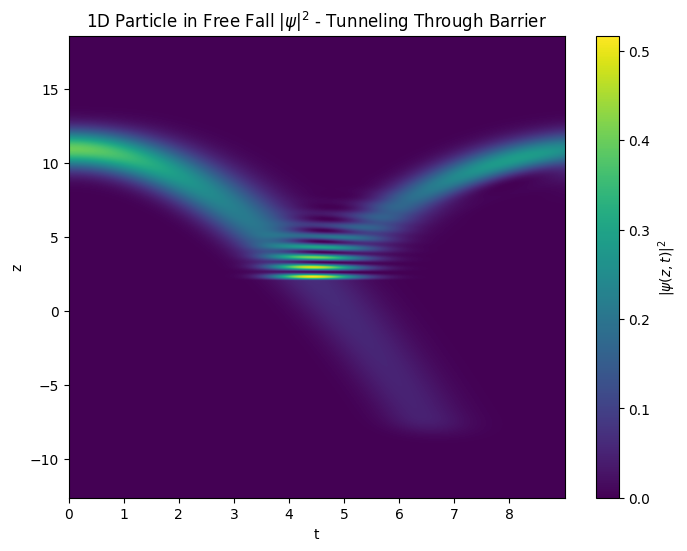
\includegraphics[width=1\linewidth]{Figures//1d_arrival_time/single_bounce.png}

    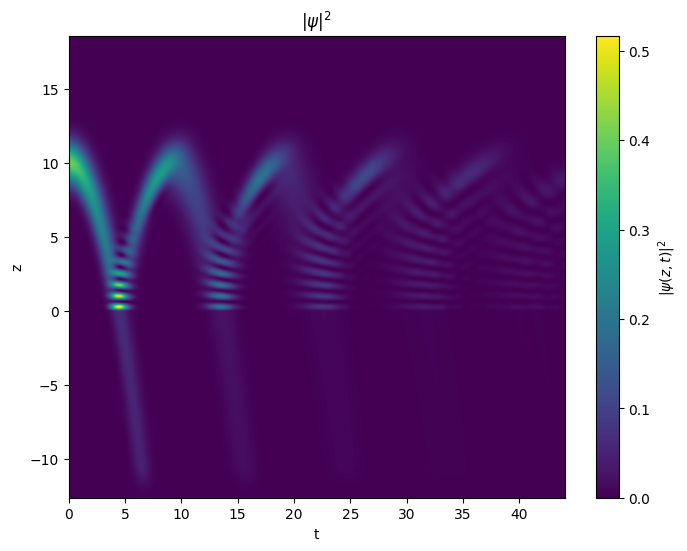
\includegraphics[width=1\linewidth]{Figures//1d_arrival_time/many_bounces.png}
    
    \caption{The quantum particle falling under free fall, the transmitted component is absorbed at the boundary of the simulation. The reflected part of the wave function falls back down to the barrier. A detector is placed at $z=-L=-5$}
    \label{fig:single_bounce}
\end{figure}

\begin{figure}
    \centering
    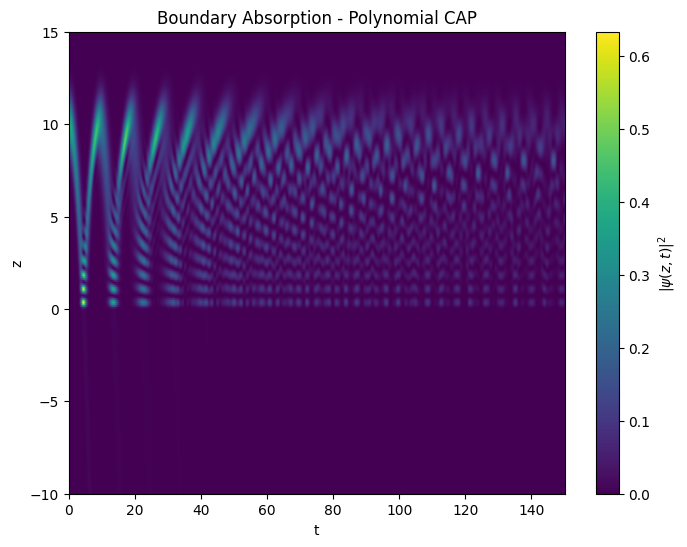
\includegraphics[width=1\linewidth]{Figures//1d_arrival_time/longterm-behaviour.png}
    \caption{A long-term run, with optimized boundary absorption coefficients, showing diffusion into a particle in a box situation, confined by a triangular barrier on one side.}
    \label{fig:long-term-run}
\end{figure}

\begin{figure}
    \centering
    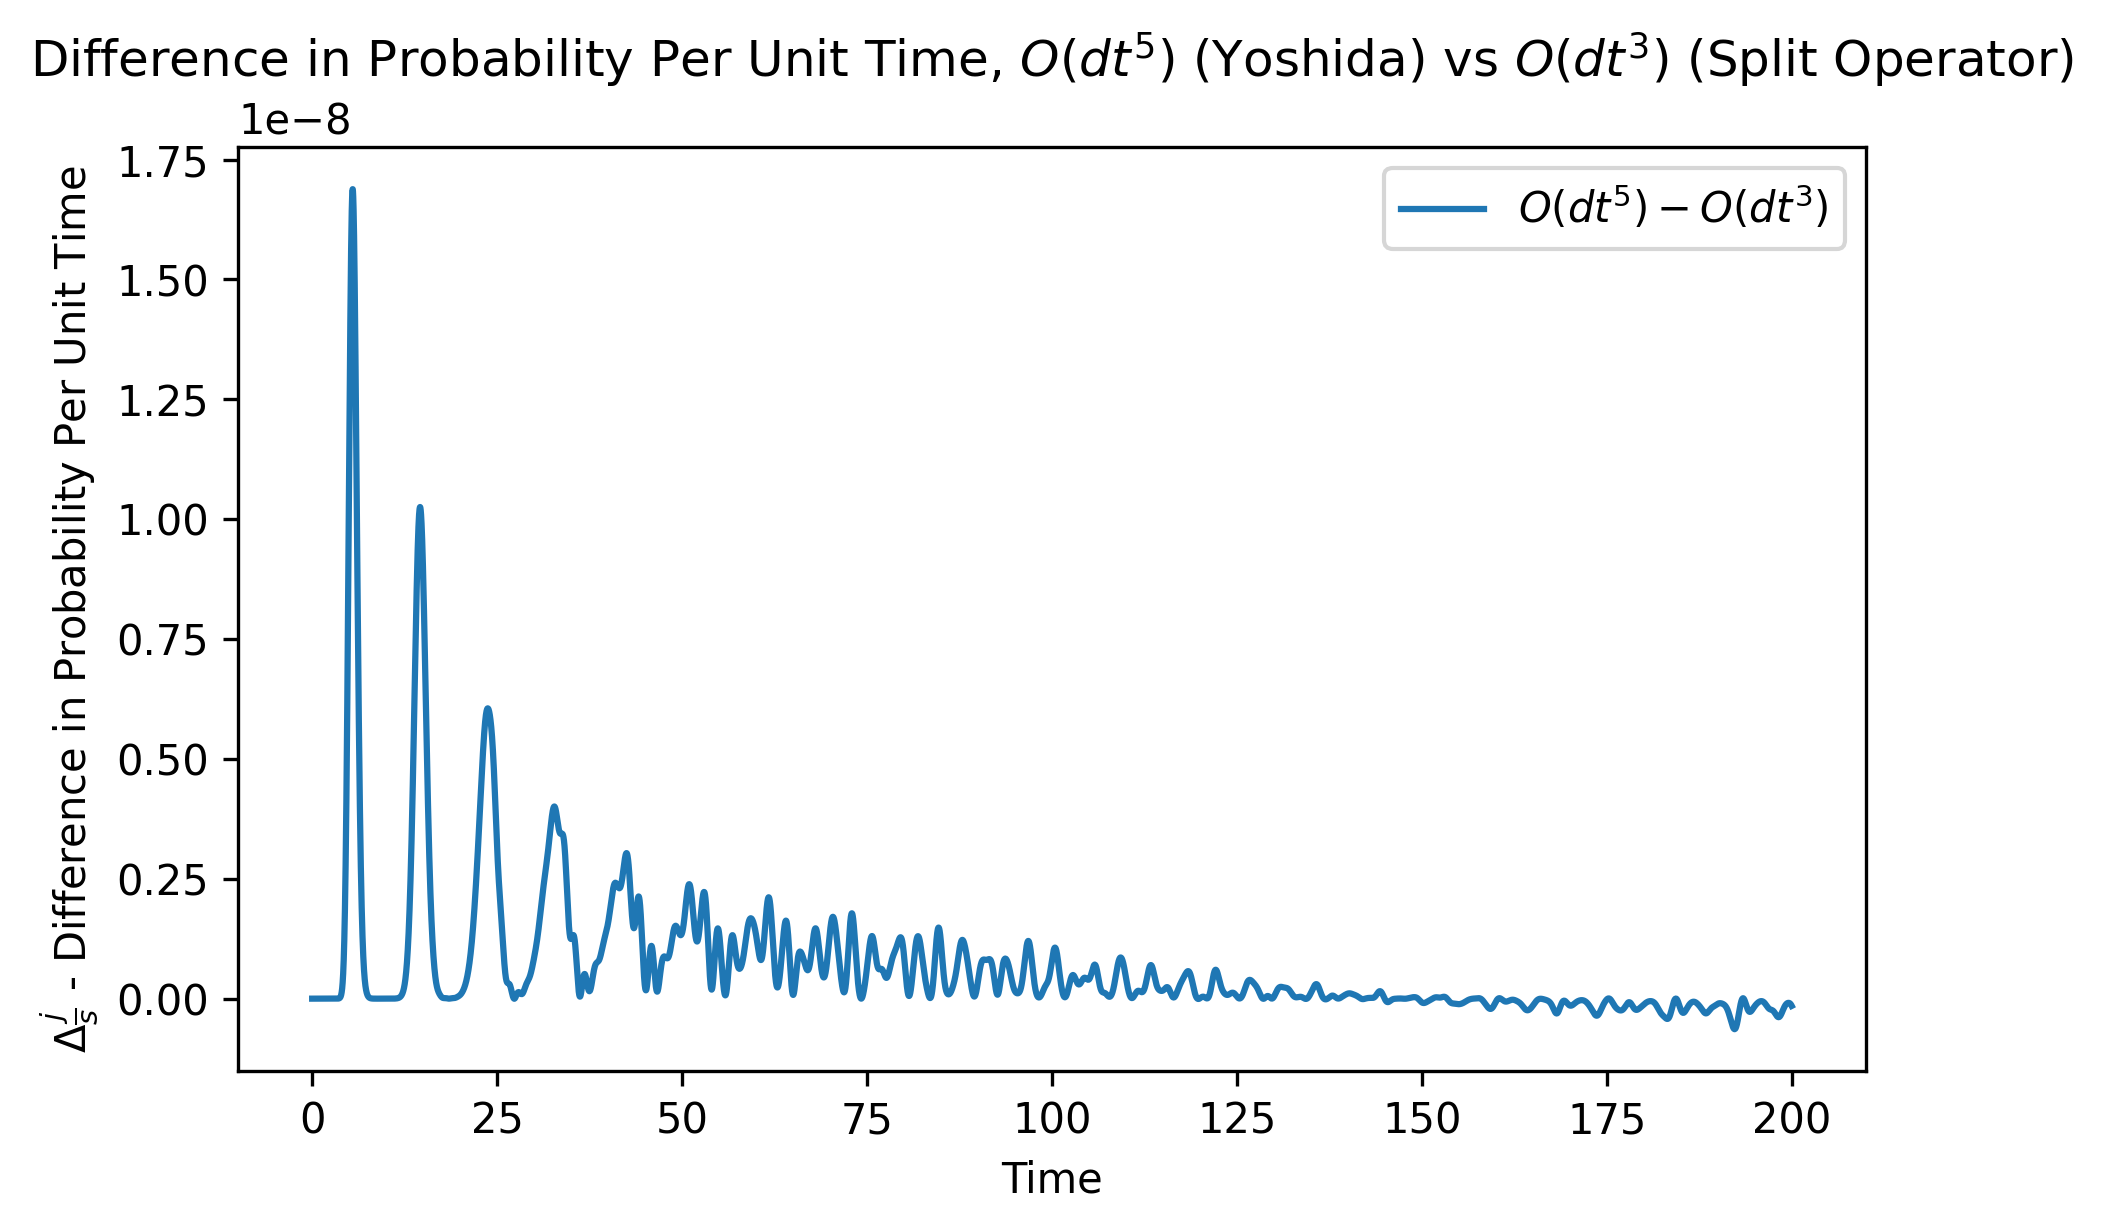
\includegraphics[width=1\linewidth]{Figures//Yoshida/ba79e062-ec65-4942-8011-72ec13c391e6.png}
    \caption{Difference in arrival time between $\bigO(dt^3)$ and $\bigO(dt^5)$ methods}
    \label{fig:difference_dt3dt5}
\end{figure}

\begin{figure}
    \centering
    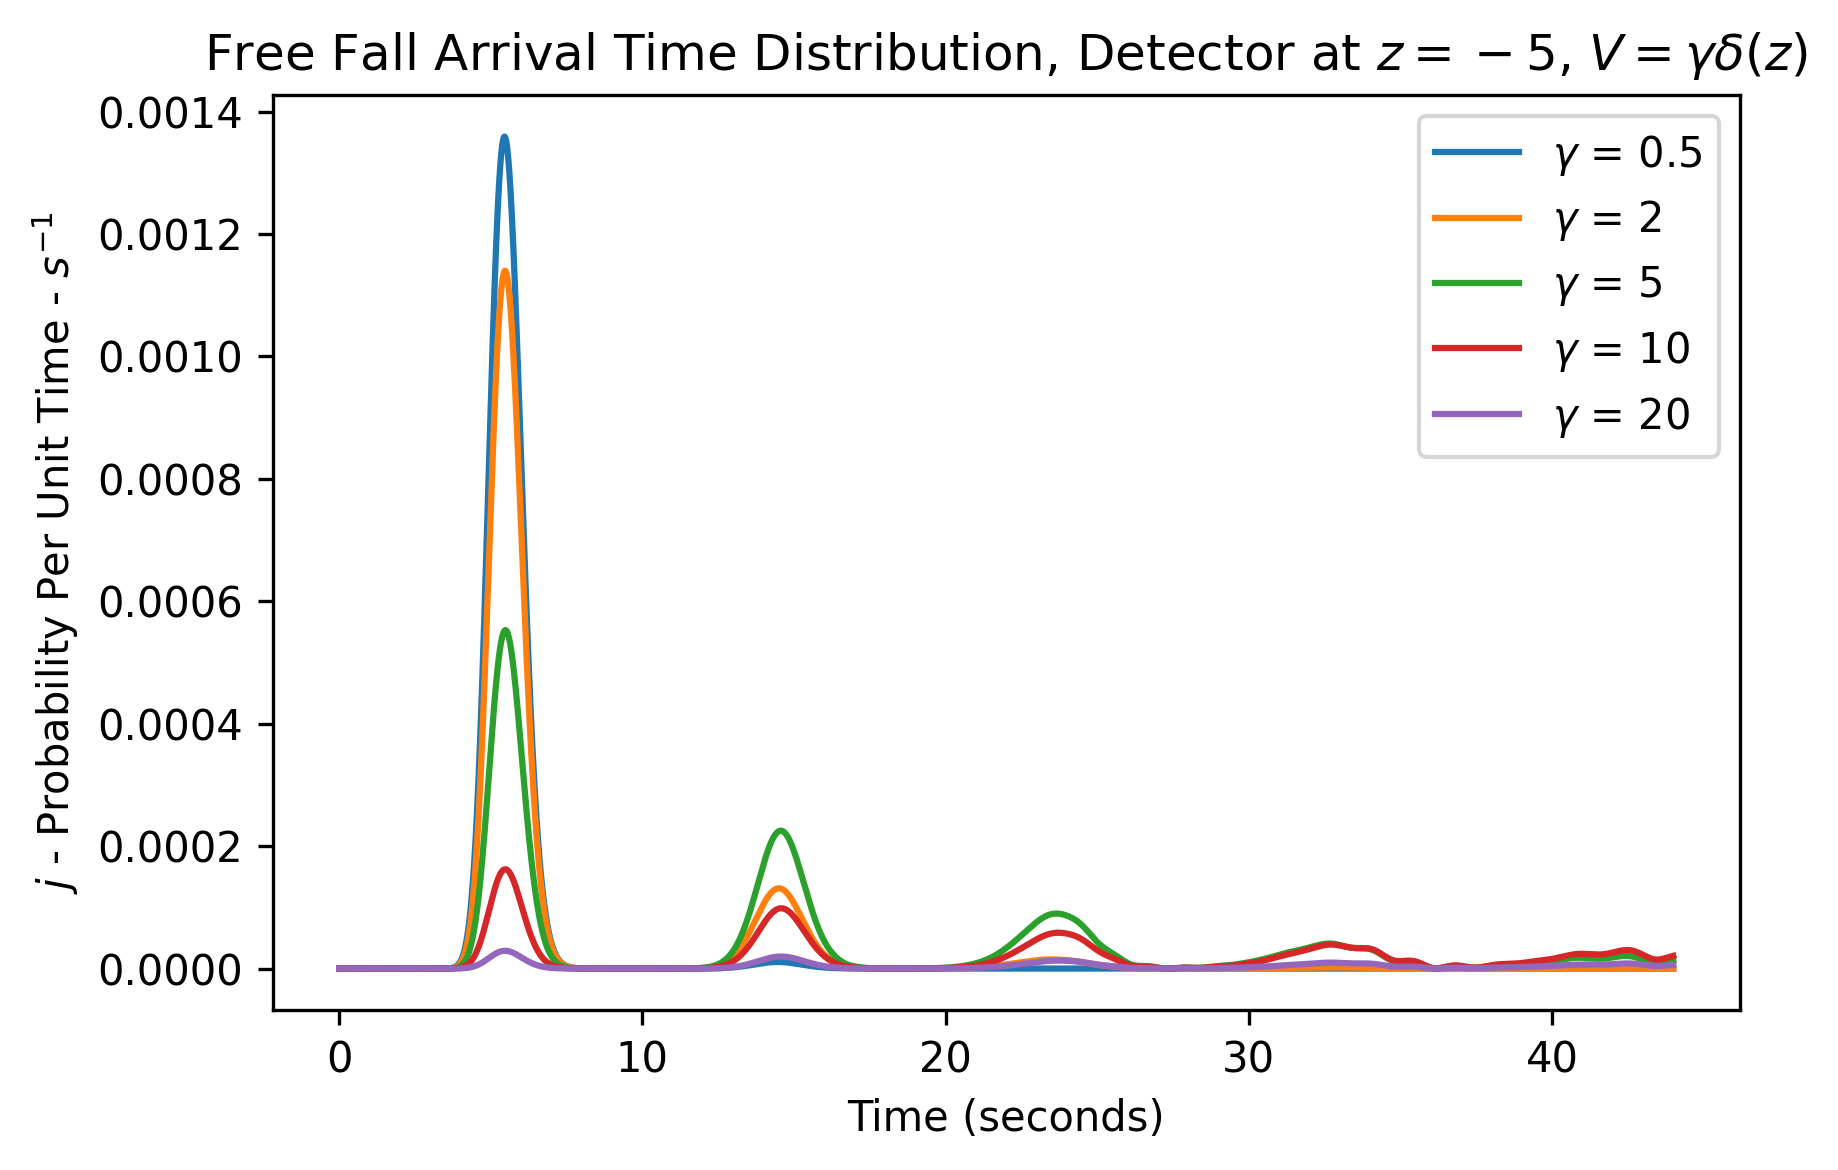
\includegraphics[width=1\linewidth]{Figures//1d_arrival_time/freefall_diff_gammas.png}
    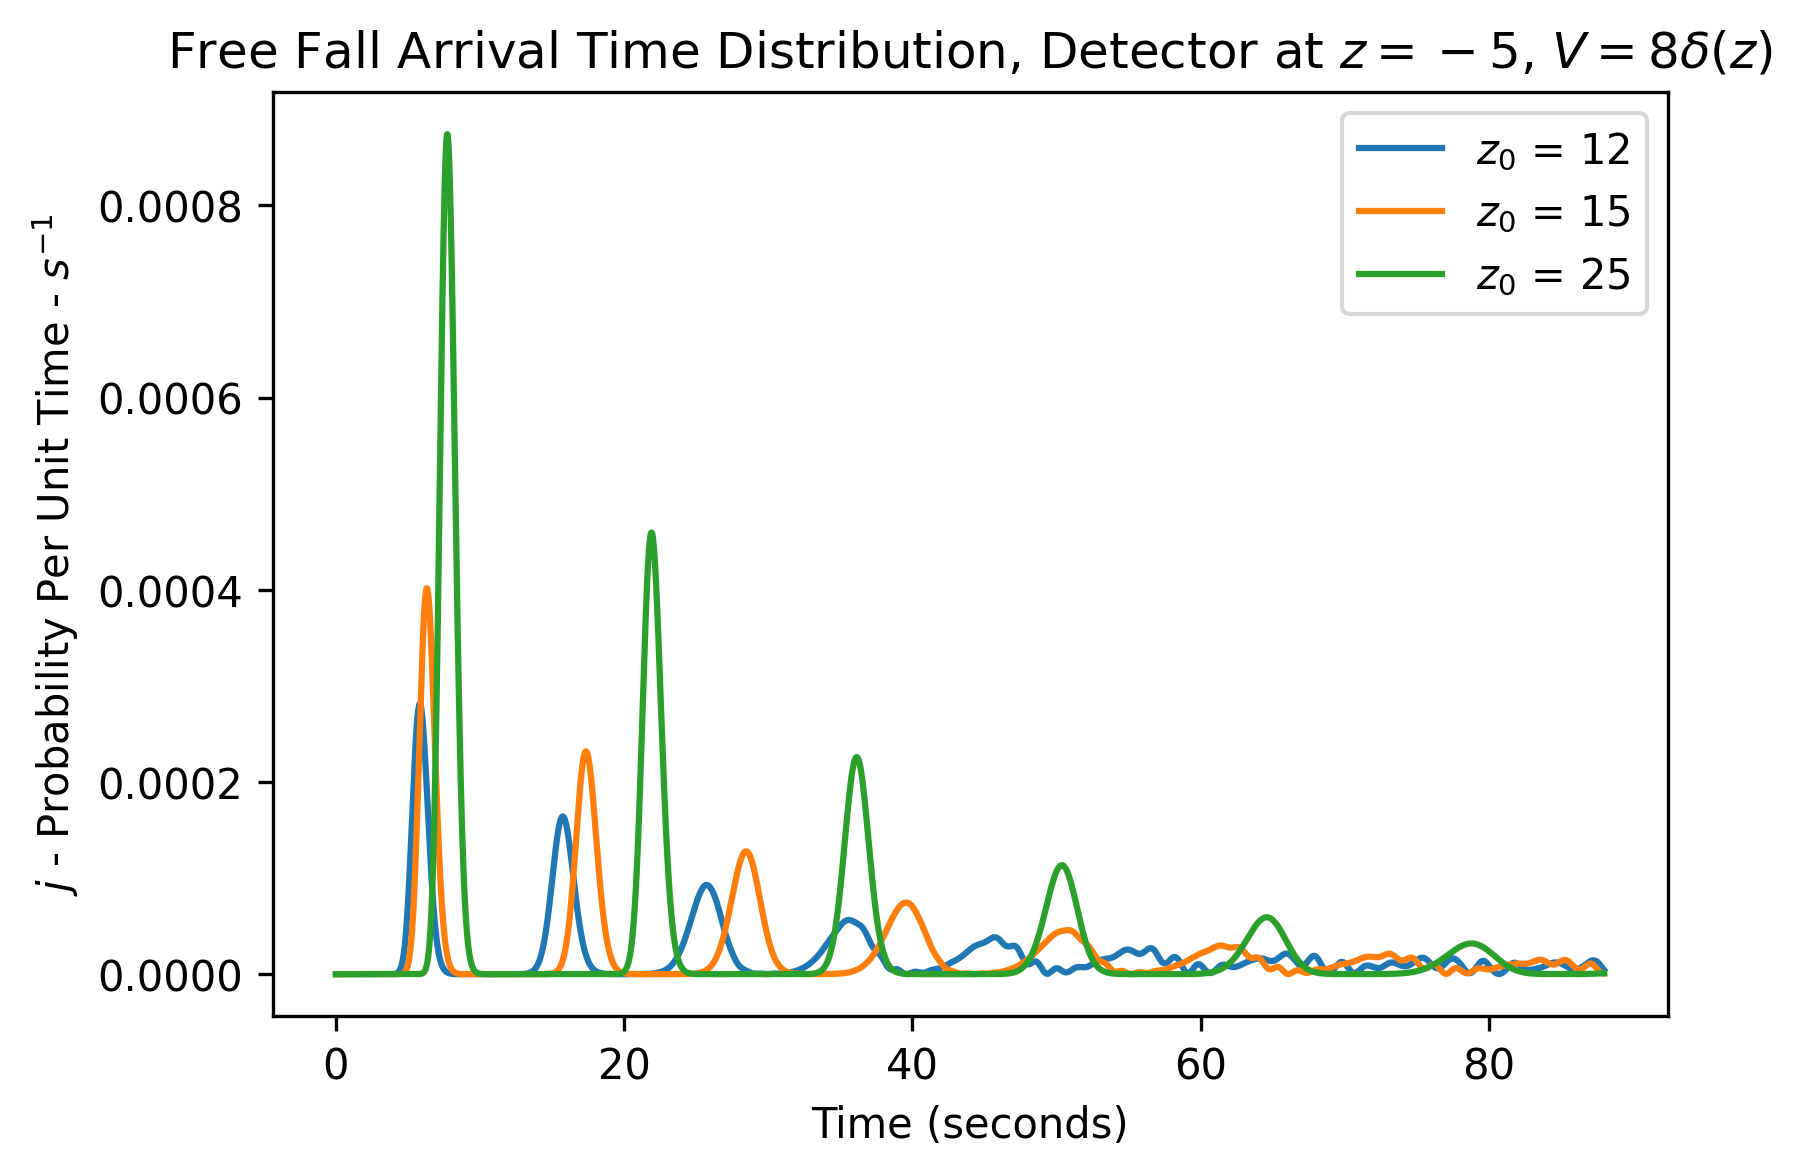
\includegraphics[width=1\linewidth]{Figures//1d_arrival_time/freefall_diff_heights.png}
    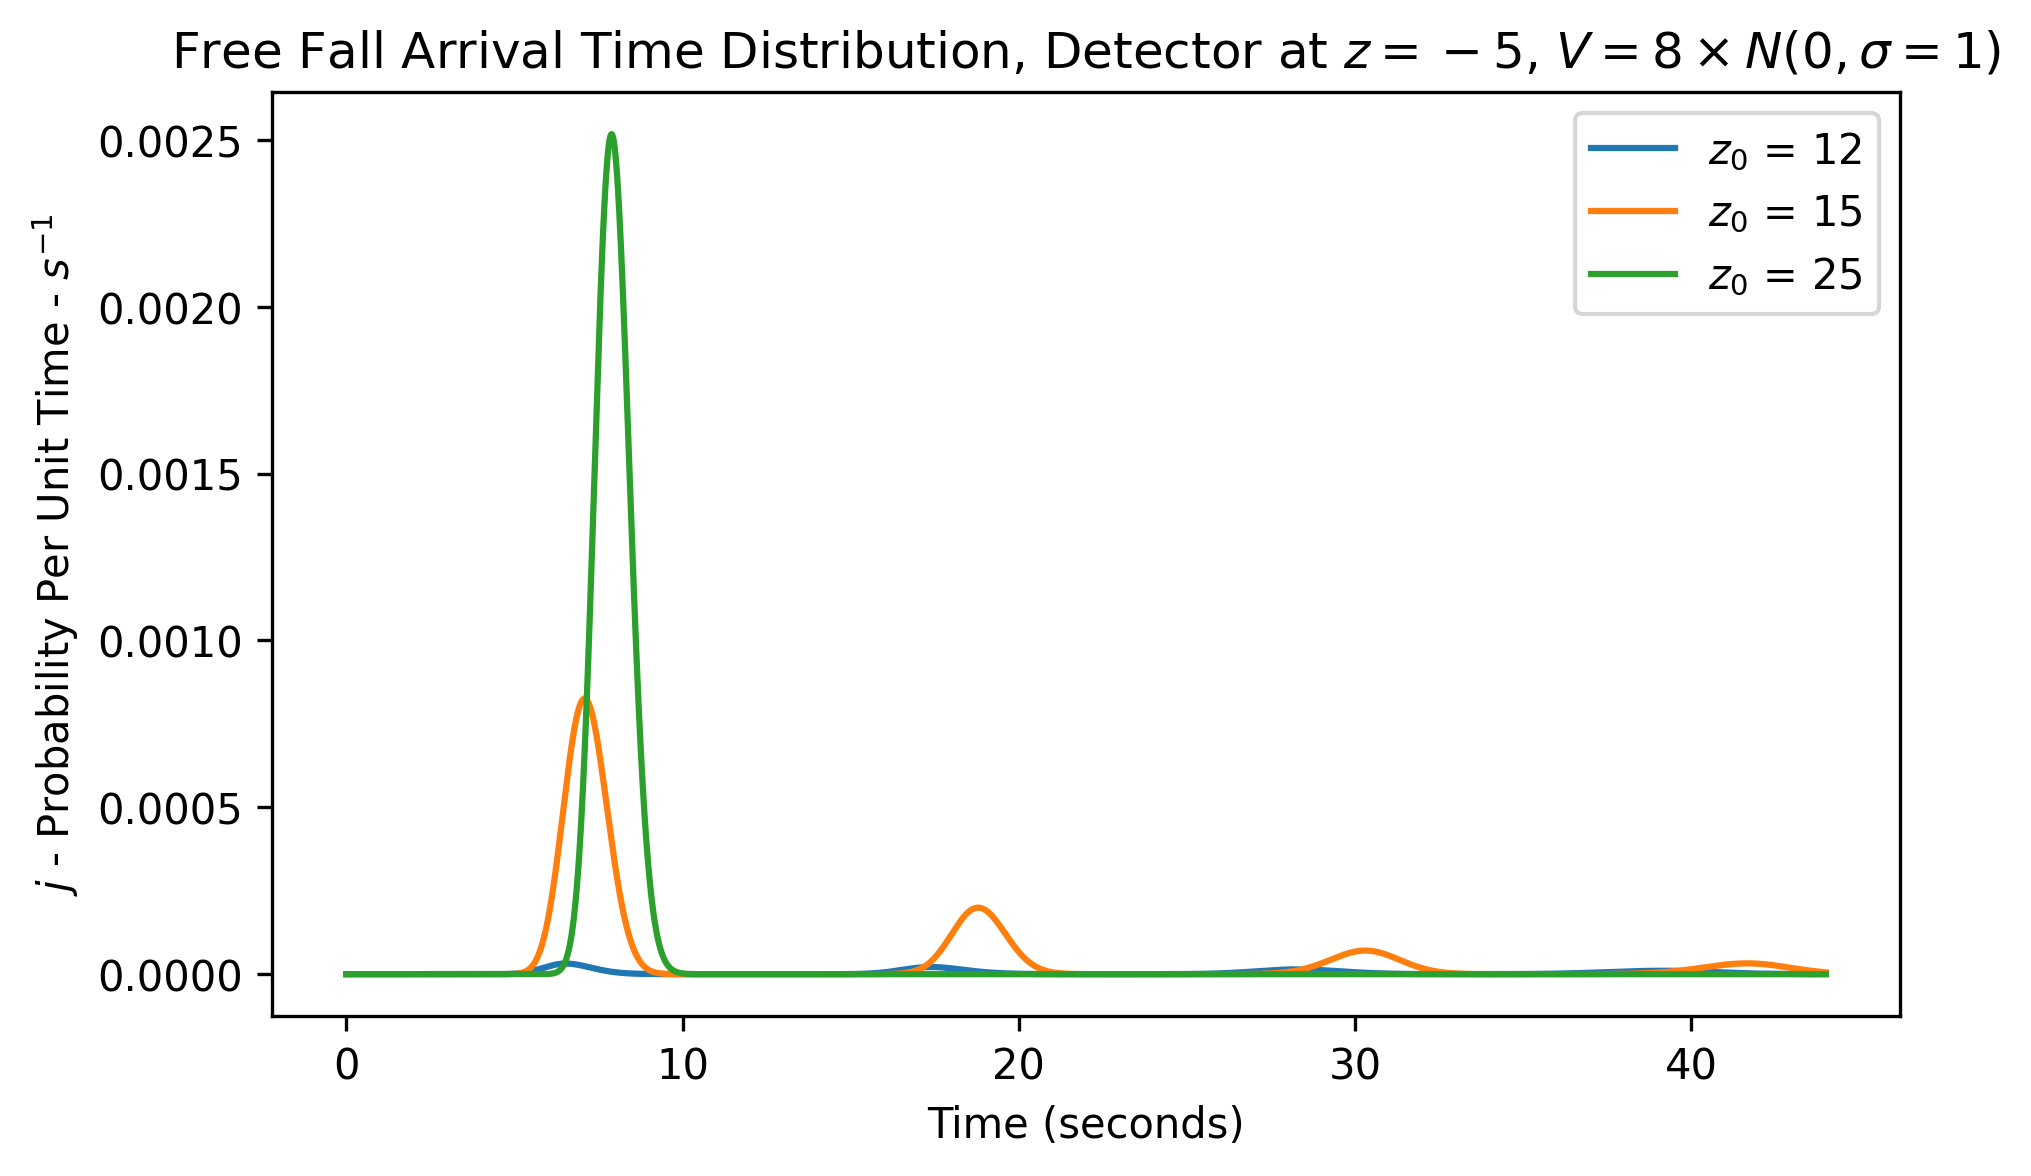
\includegraphics[width=1\linewidth]{Figures//1d_arrival_time/freefall_gaussian_different.png}
    \caption{Arrival Time Distribution with a $\gamma \delta$ barrier, at different gamma barrier strengths. There's a clear regularity to be spotted here, that's not observed with Gaussian barriers.}
    \label{fig:arrival_time_freefall_diff_gammas}
\end{figure}

\begin{figure}
    \centering
    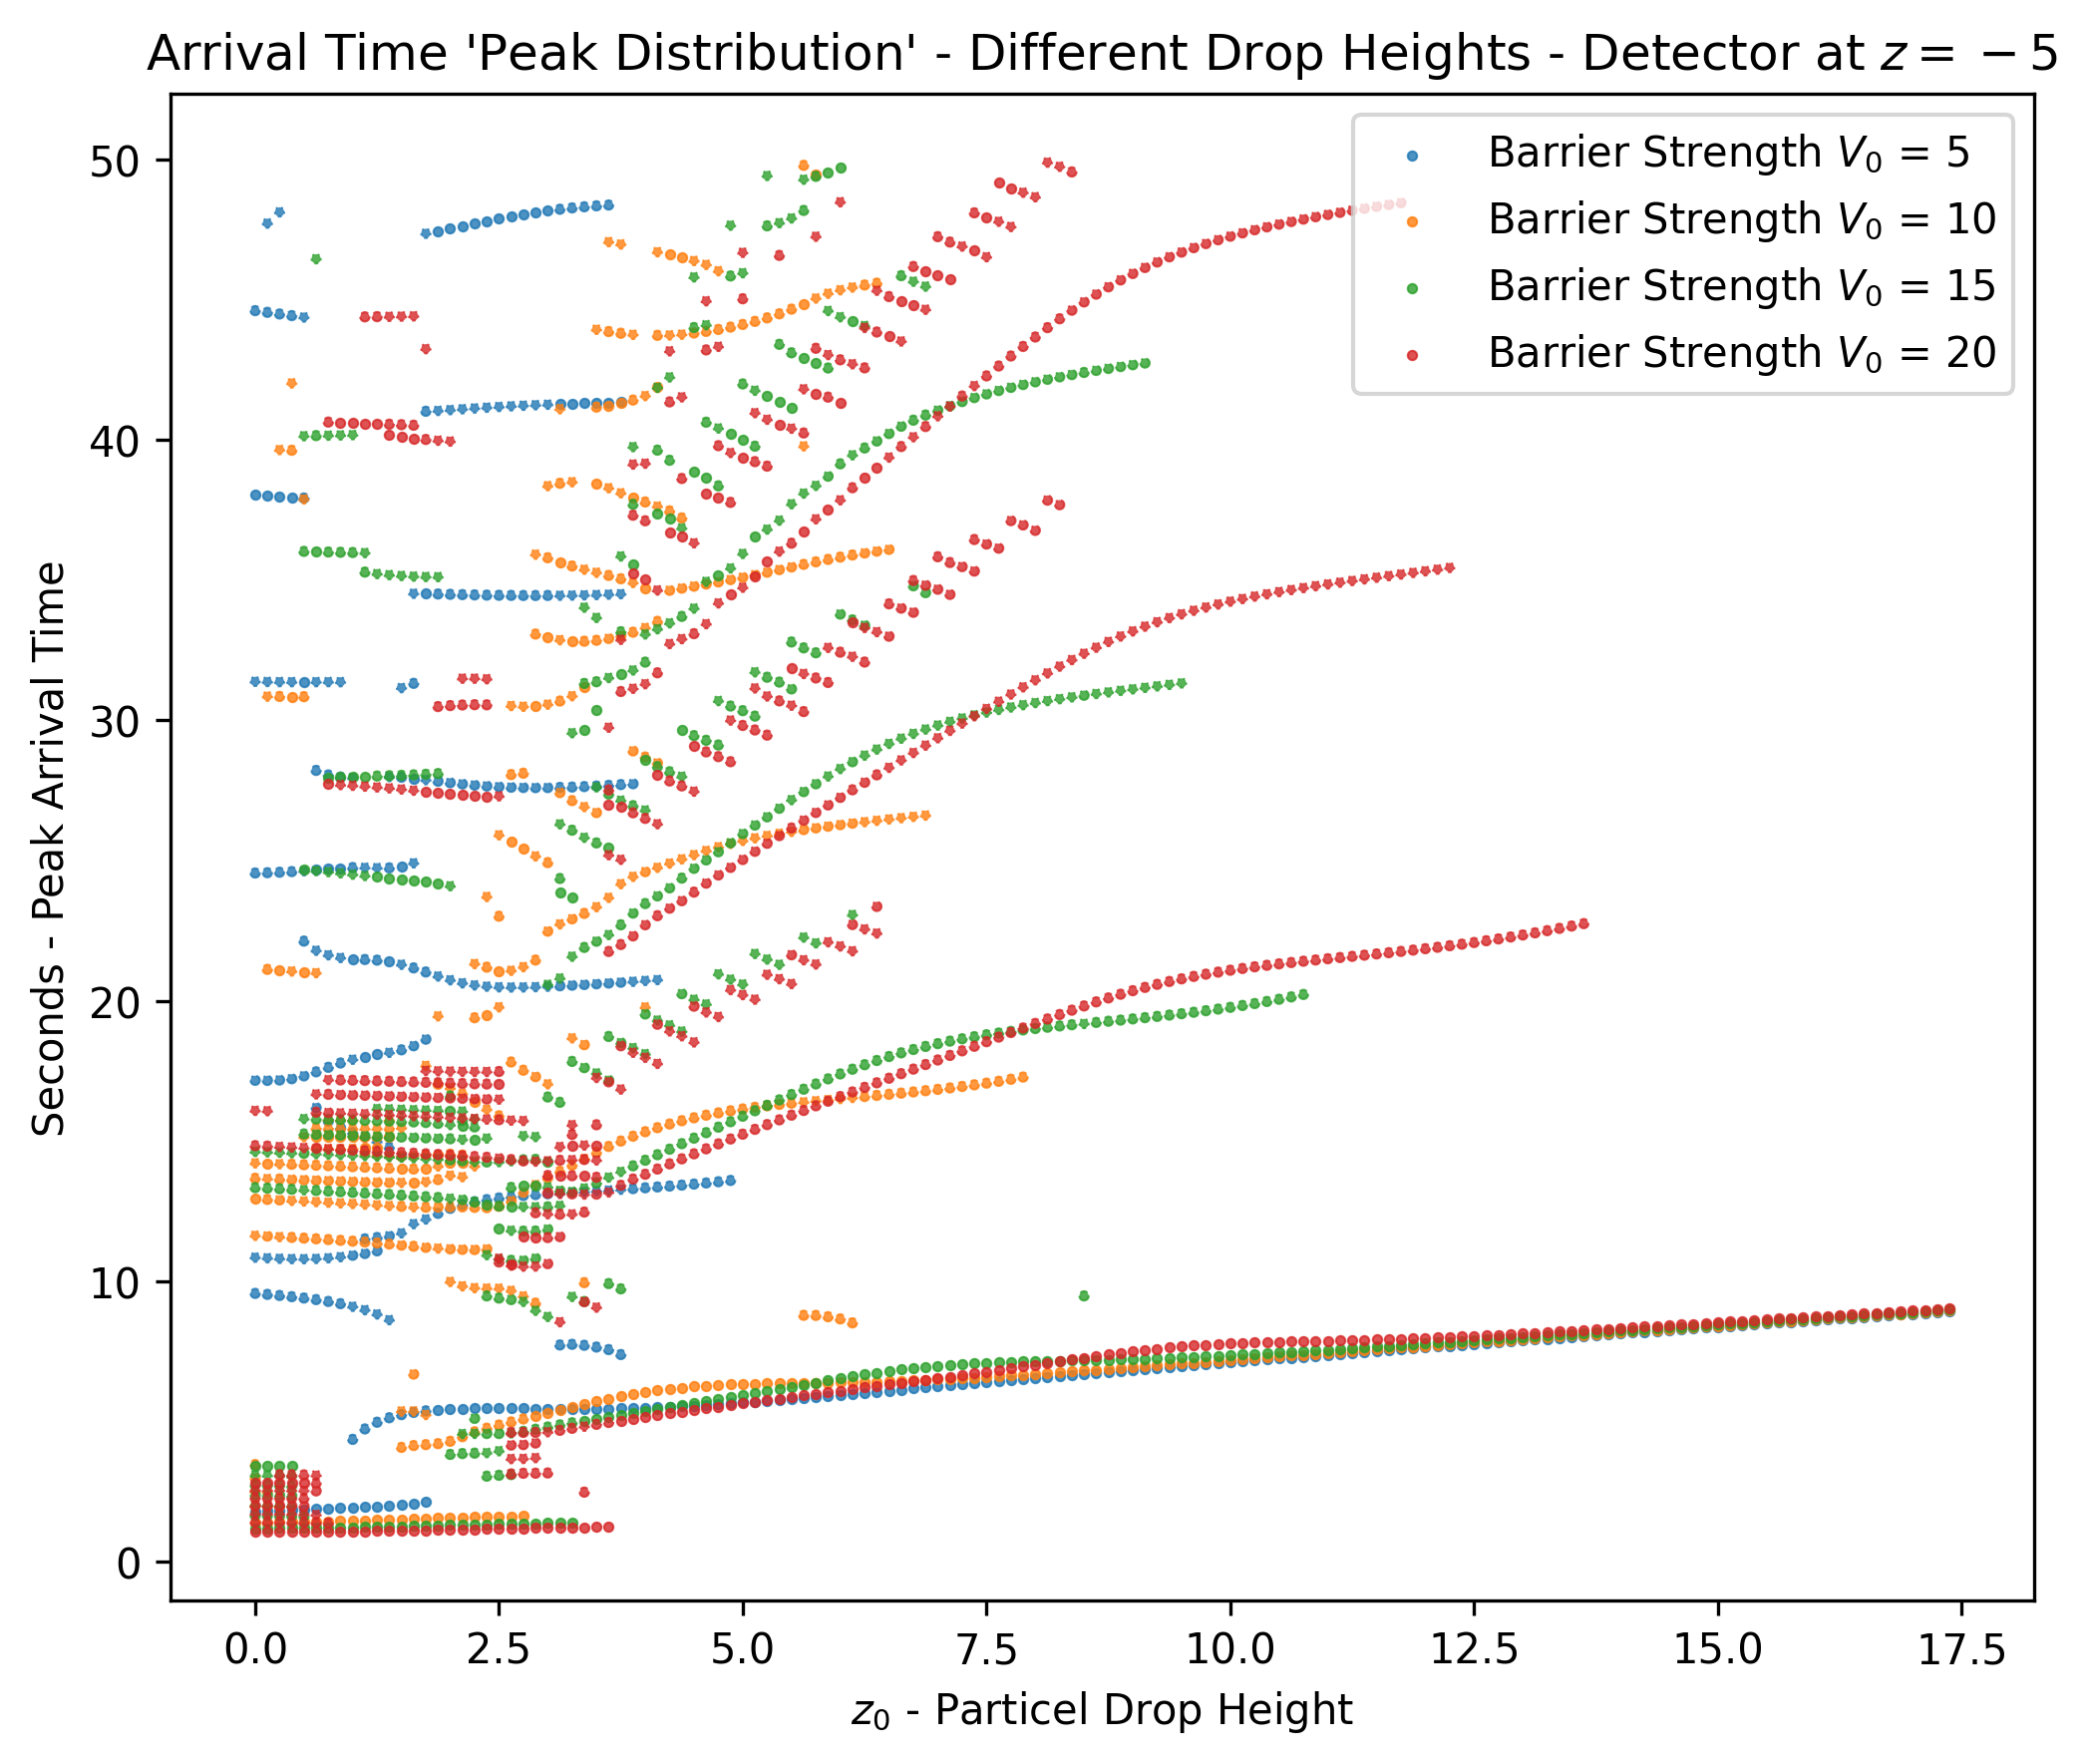
\includegraphics[width=1\linewidth]{Figures//Yoshida/c8e61b3f-c0e7-42e2-9757-332081859752.png}
    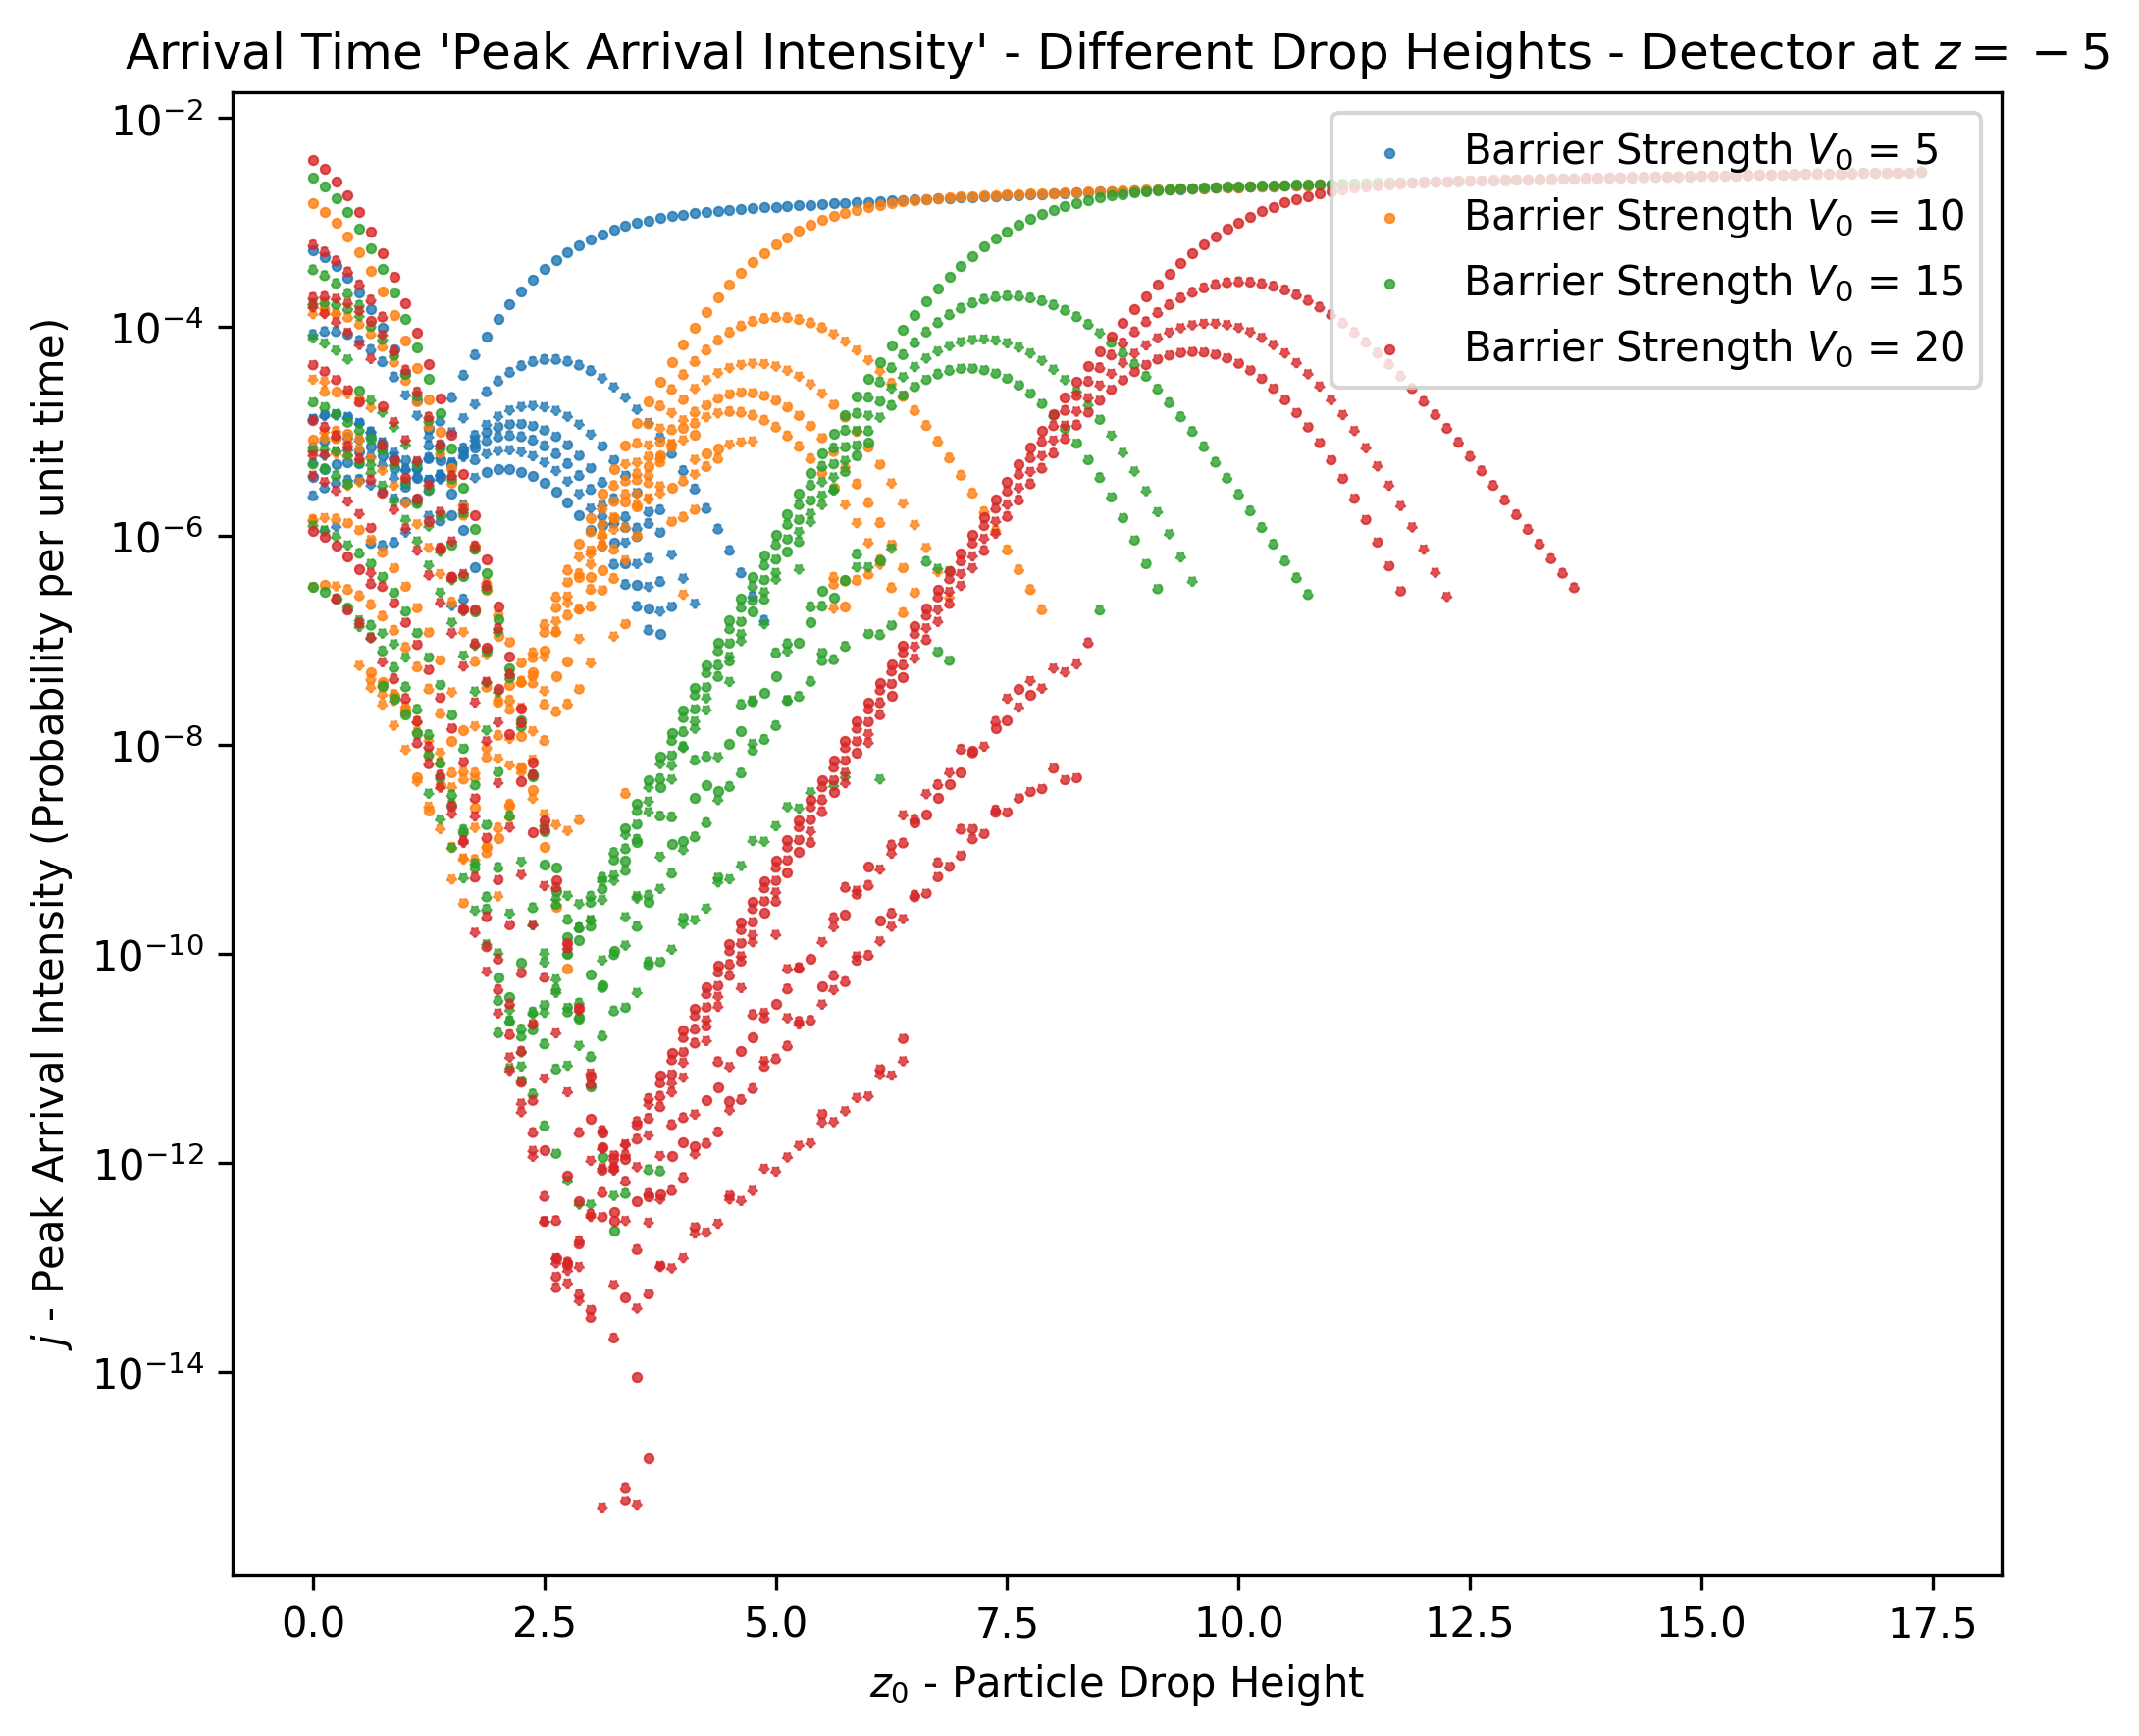
\includegraphics[width=1\linewidth]{Figures//Yoshida/eb253fe9-8277-4b3a-ab94-bbfb6369647d.png}
    \caption{Peaks in Arrival Time Distribution. Each experiment is done at different drop heights (x-axis), and colored according to different barrier strengths. Notice the "continuous" and "chartered" regions in the upper graph starting from drop height 5, and 15 and 20 magnetic units. On the lower graph, notice the asymptotic behaviour of intensity of the first bounce, and the parabola-like drop-off for each subsequent bounce as the particle is dropped from higher heights.}
    \label{fig:particle_drop_height_power}
\end{figure}

\begin{figure}
    \centering
    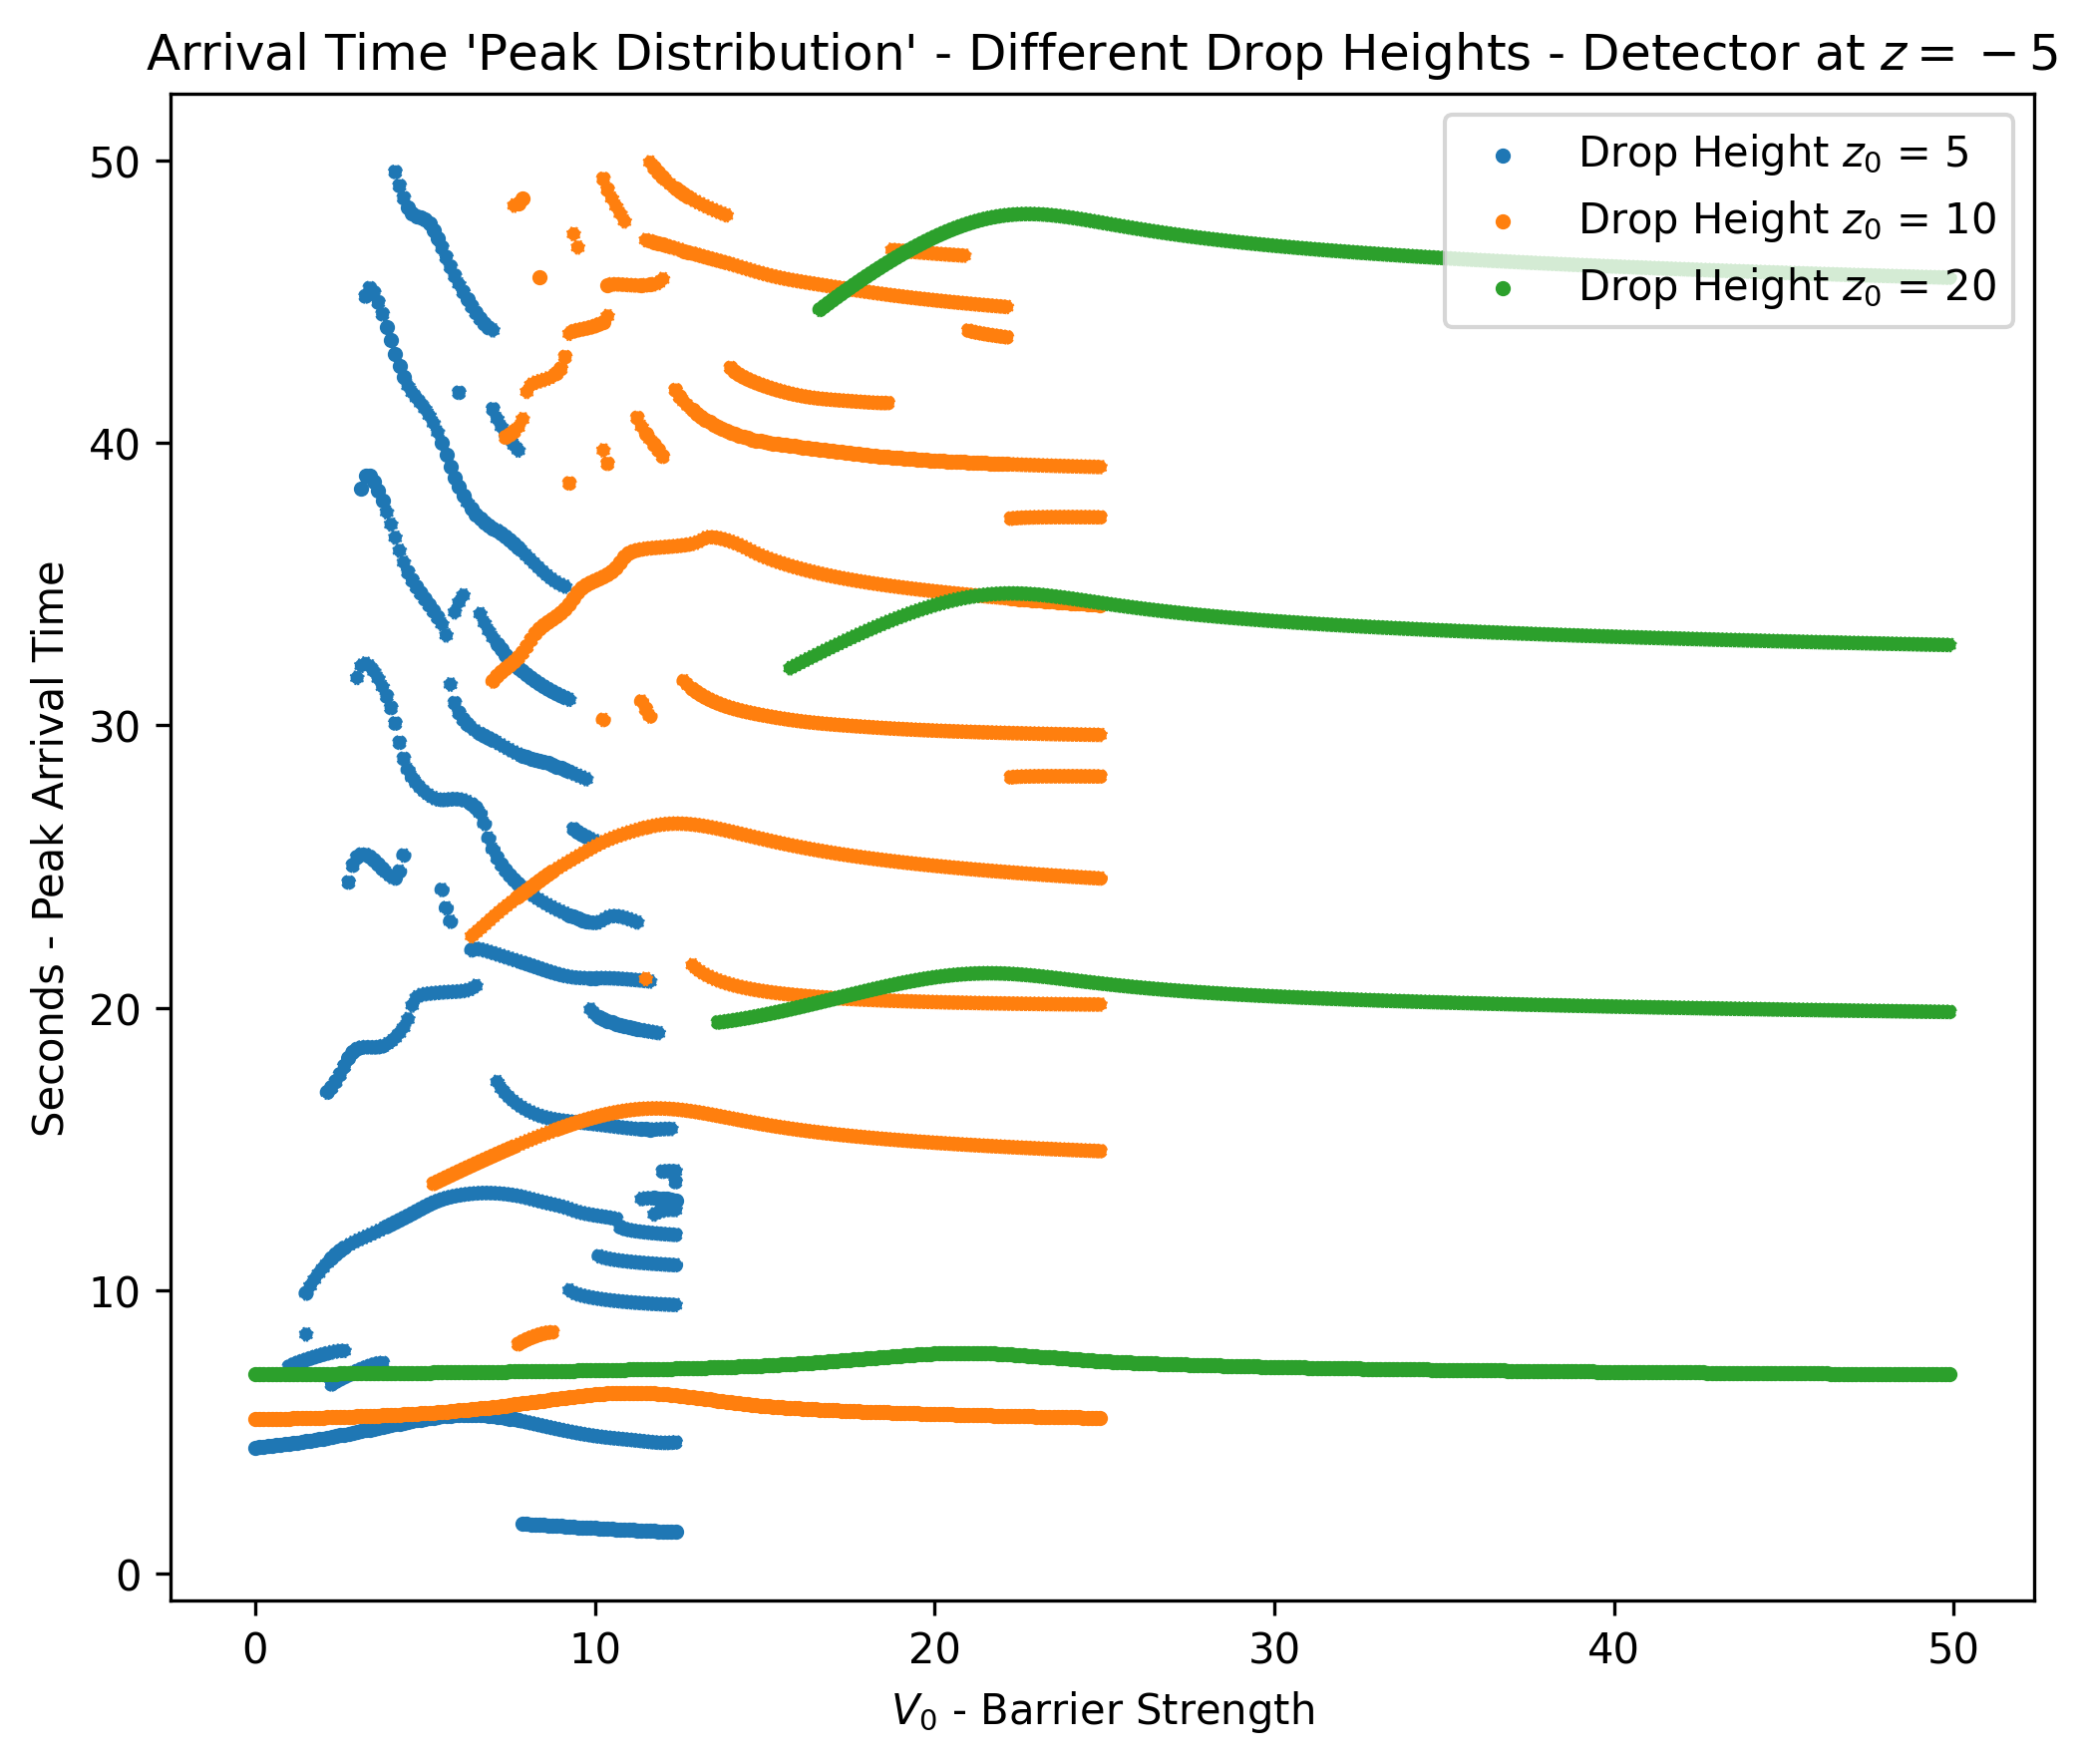
\includegraphics[width=1\linewidth]{Figures//Yoshida/6663e0ce-fb89-4819-b390-3bad6ba0e3c4.png}
    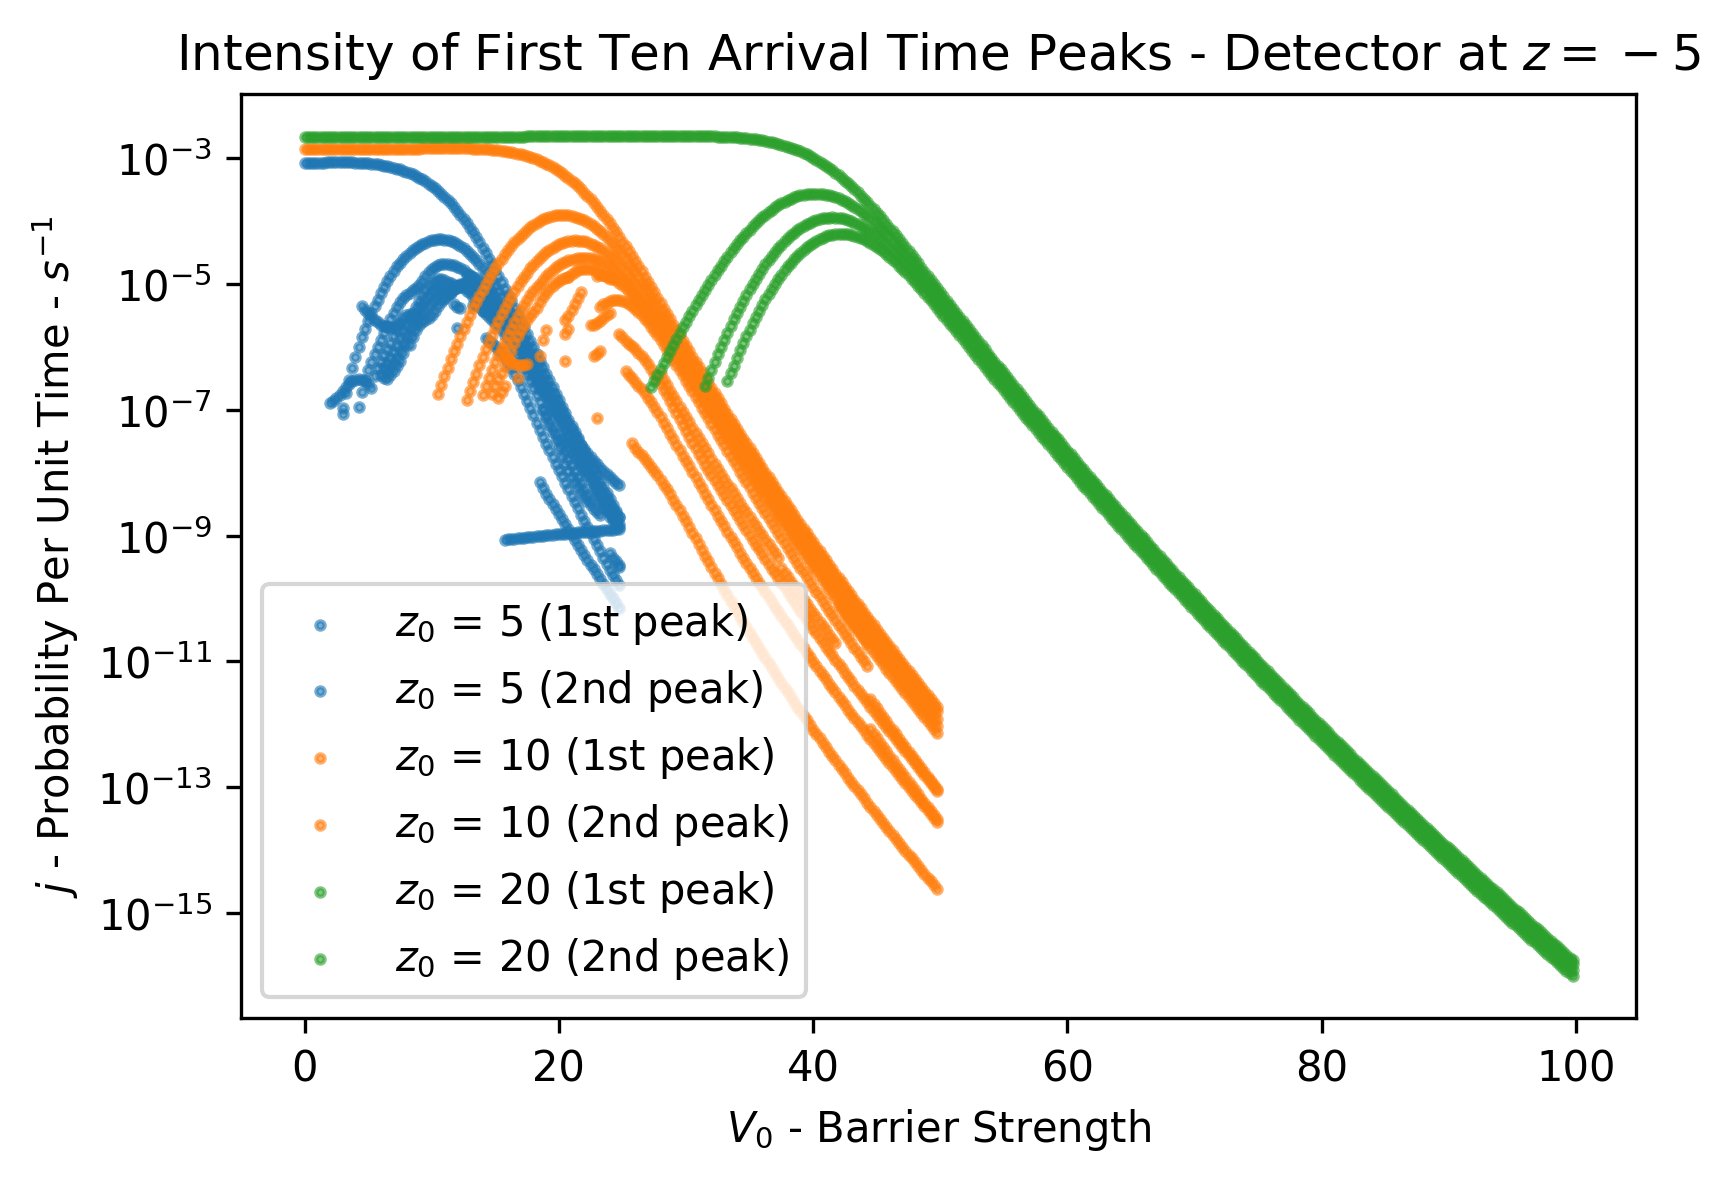
\includegraphics[width=1\linewidth]{Figures//Yoshida/2897f6b7-dd93-43e5-8846-e3fb0f150b28.png}
    \caption{Peaks in Arrival Time Distribution for Gaussian barriers. Each simulated experiment is done at different barrier strength (x-axis), and colored according to different drop heights. The upper chart plots arrival times (seconds) in function of barrier strength, whereas the lower chart plots arrival time intensities in function of barrier strength. Notice the band structure formation in the low barrier strength region on the upper graph. On the lower graph, notice the asymptotically decreasing intensity as the strength of the barrier increases.}
    \label{fig:particklesupser_strength}
\end{figure}

% delta simulations
\begin{figure
    \centering
    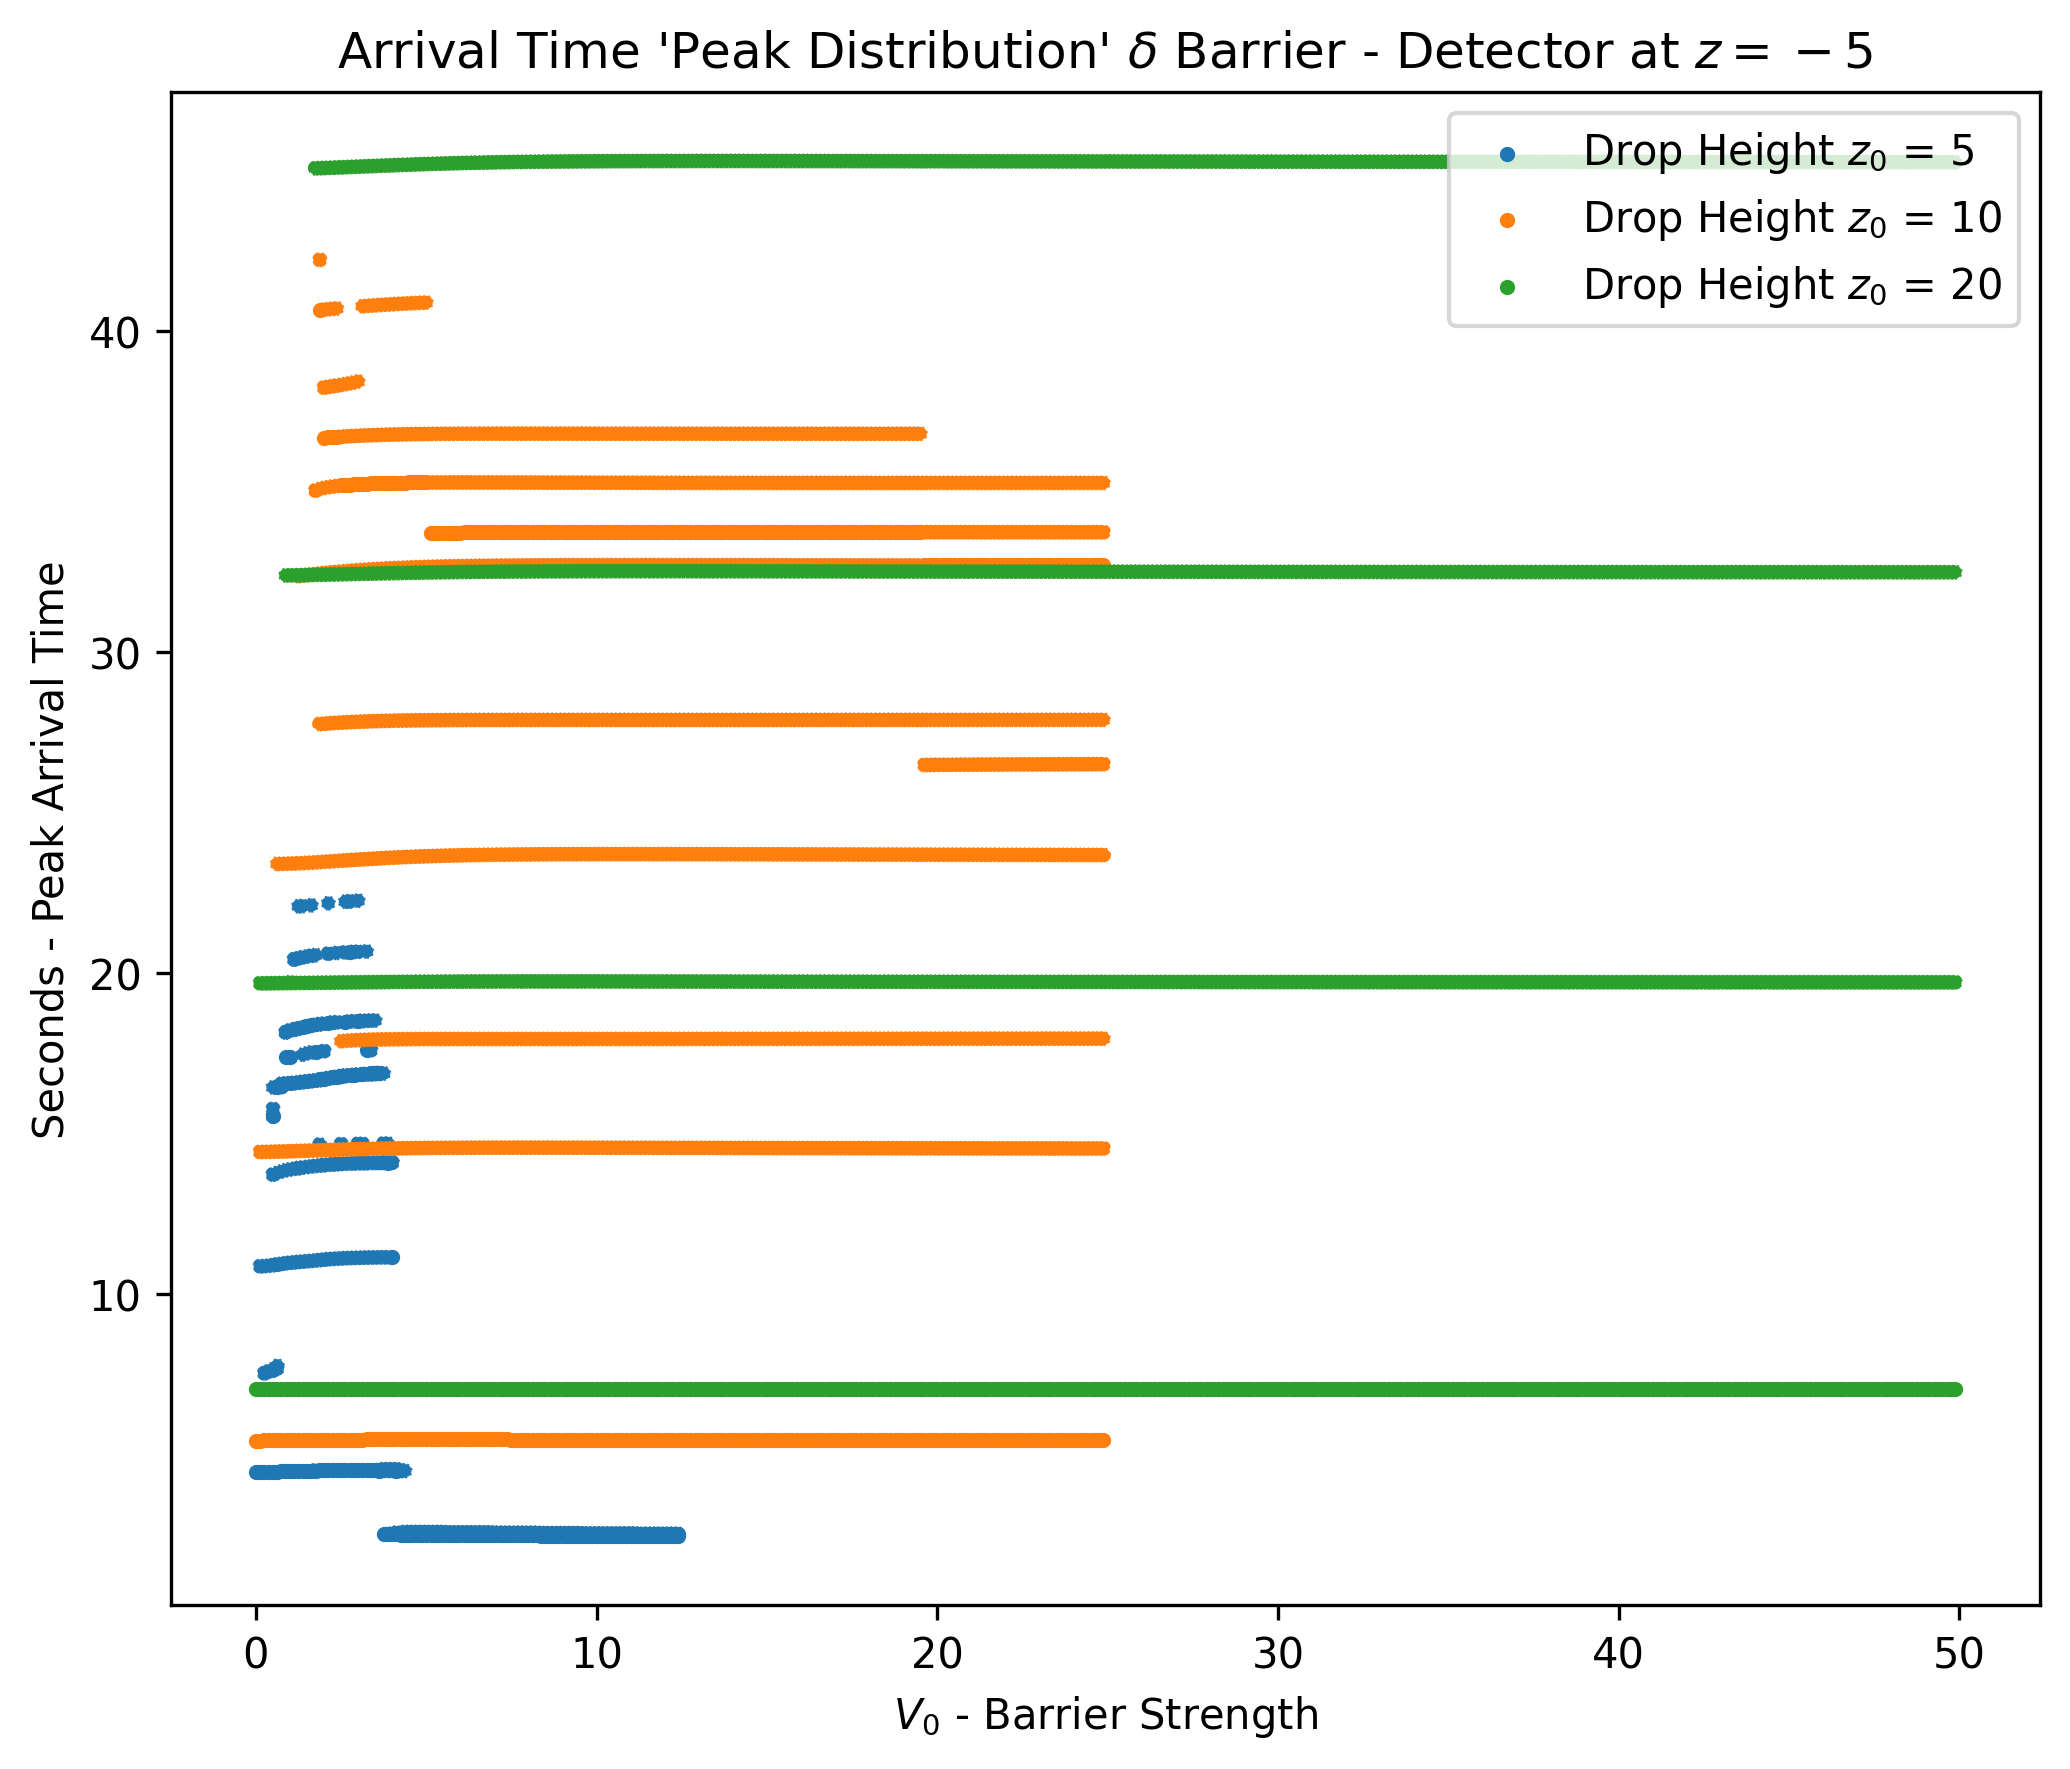
\includegraphics[width=1\linewidth]{Figures//Yoshida/7d42f617-724e-4ce1-9783-f4b1483645be.png}
    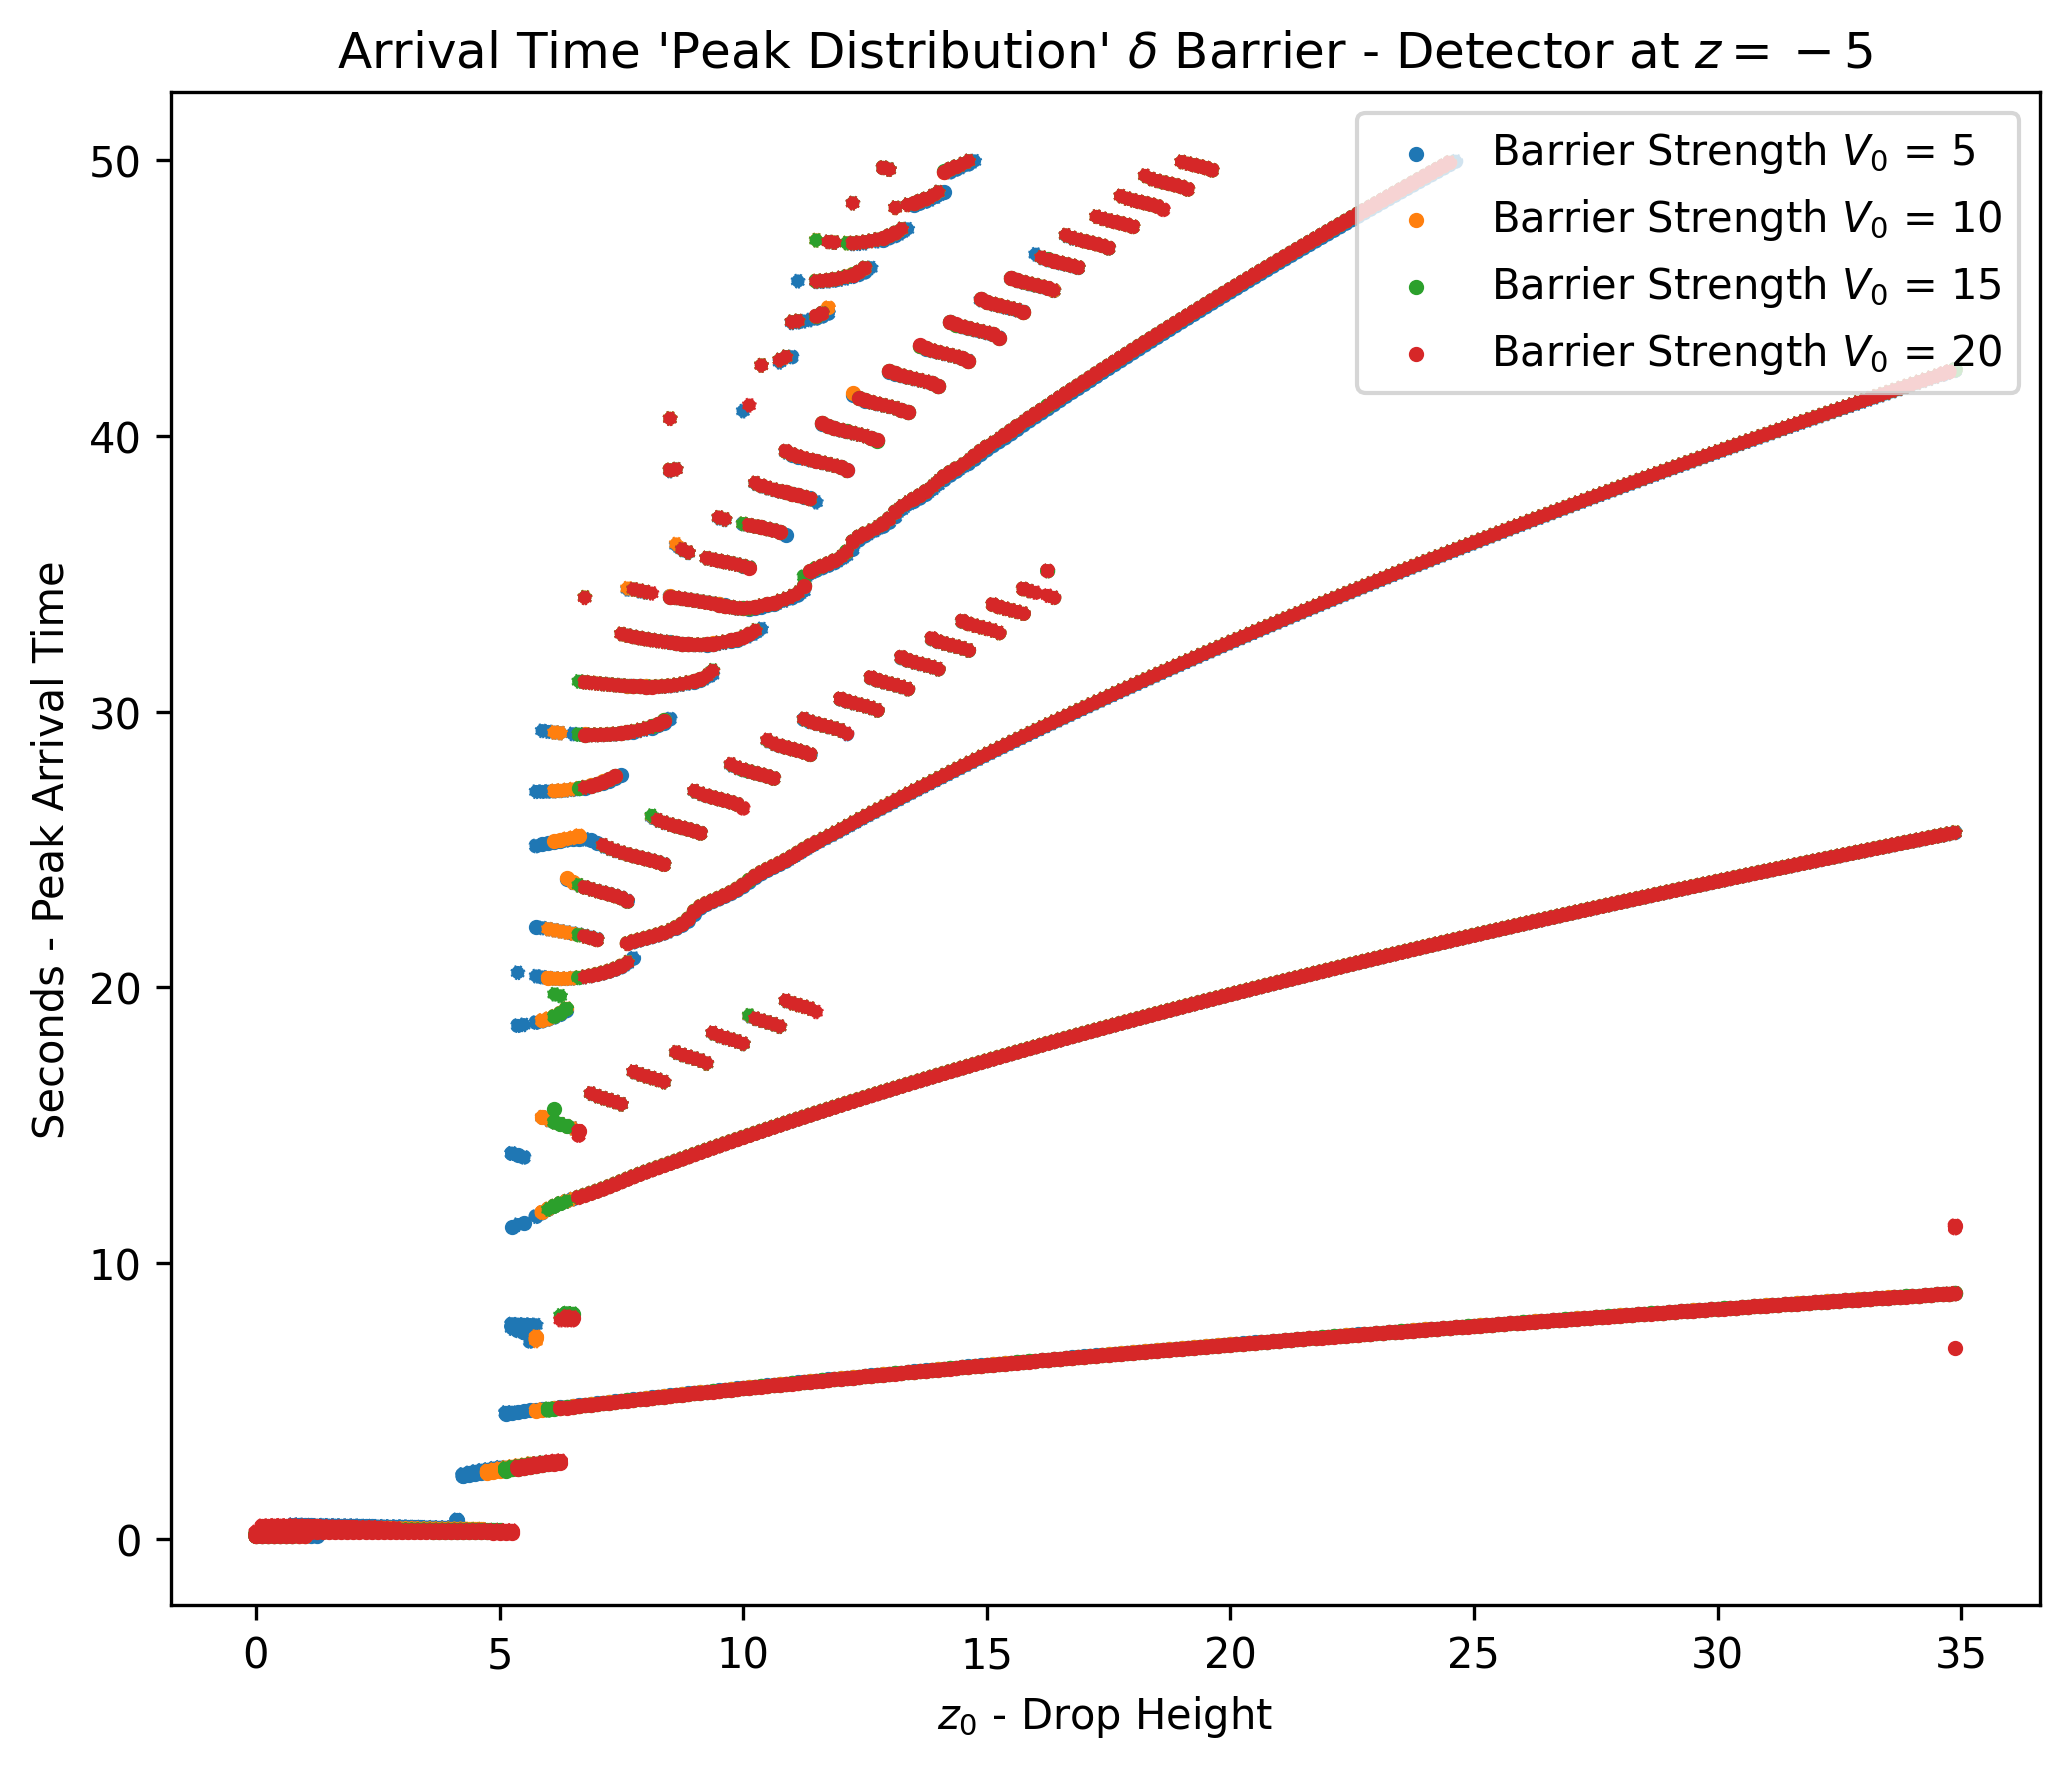
\includegraphics[width=1\linewidth]{Figures//Yoshida/595bccd4-04d1-497f-b897-40bc0226430c.png}
    \caption{Peaks in Arrival Time \textbf{(seconds)} Distribution for a Delta barrier. Notice the regularity of arrival times in the upper chart, making the delta barrier approximate to semi-classical predictions, which need further in depth considerations. On the lower graph, it's clearly seen that regardless of barrier strength, the four situations produce the same peak distribution in seconds, except for the transitionary region at 5 units in drop height.}
    \label{fig:deltamega_gazon}
\end{figure}

\begin{figure}
    \centering
    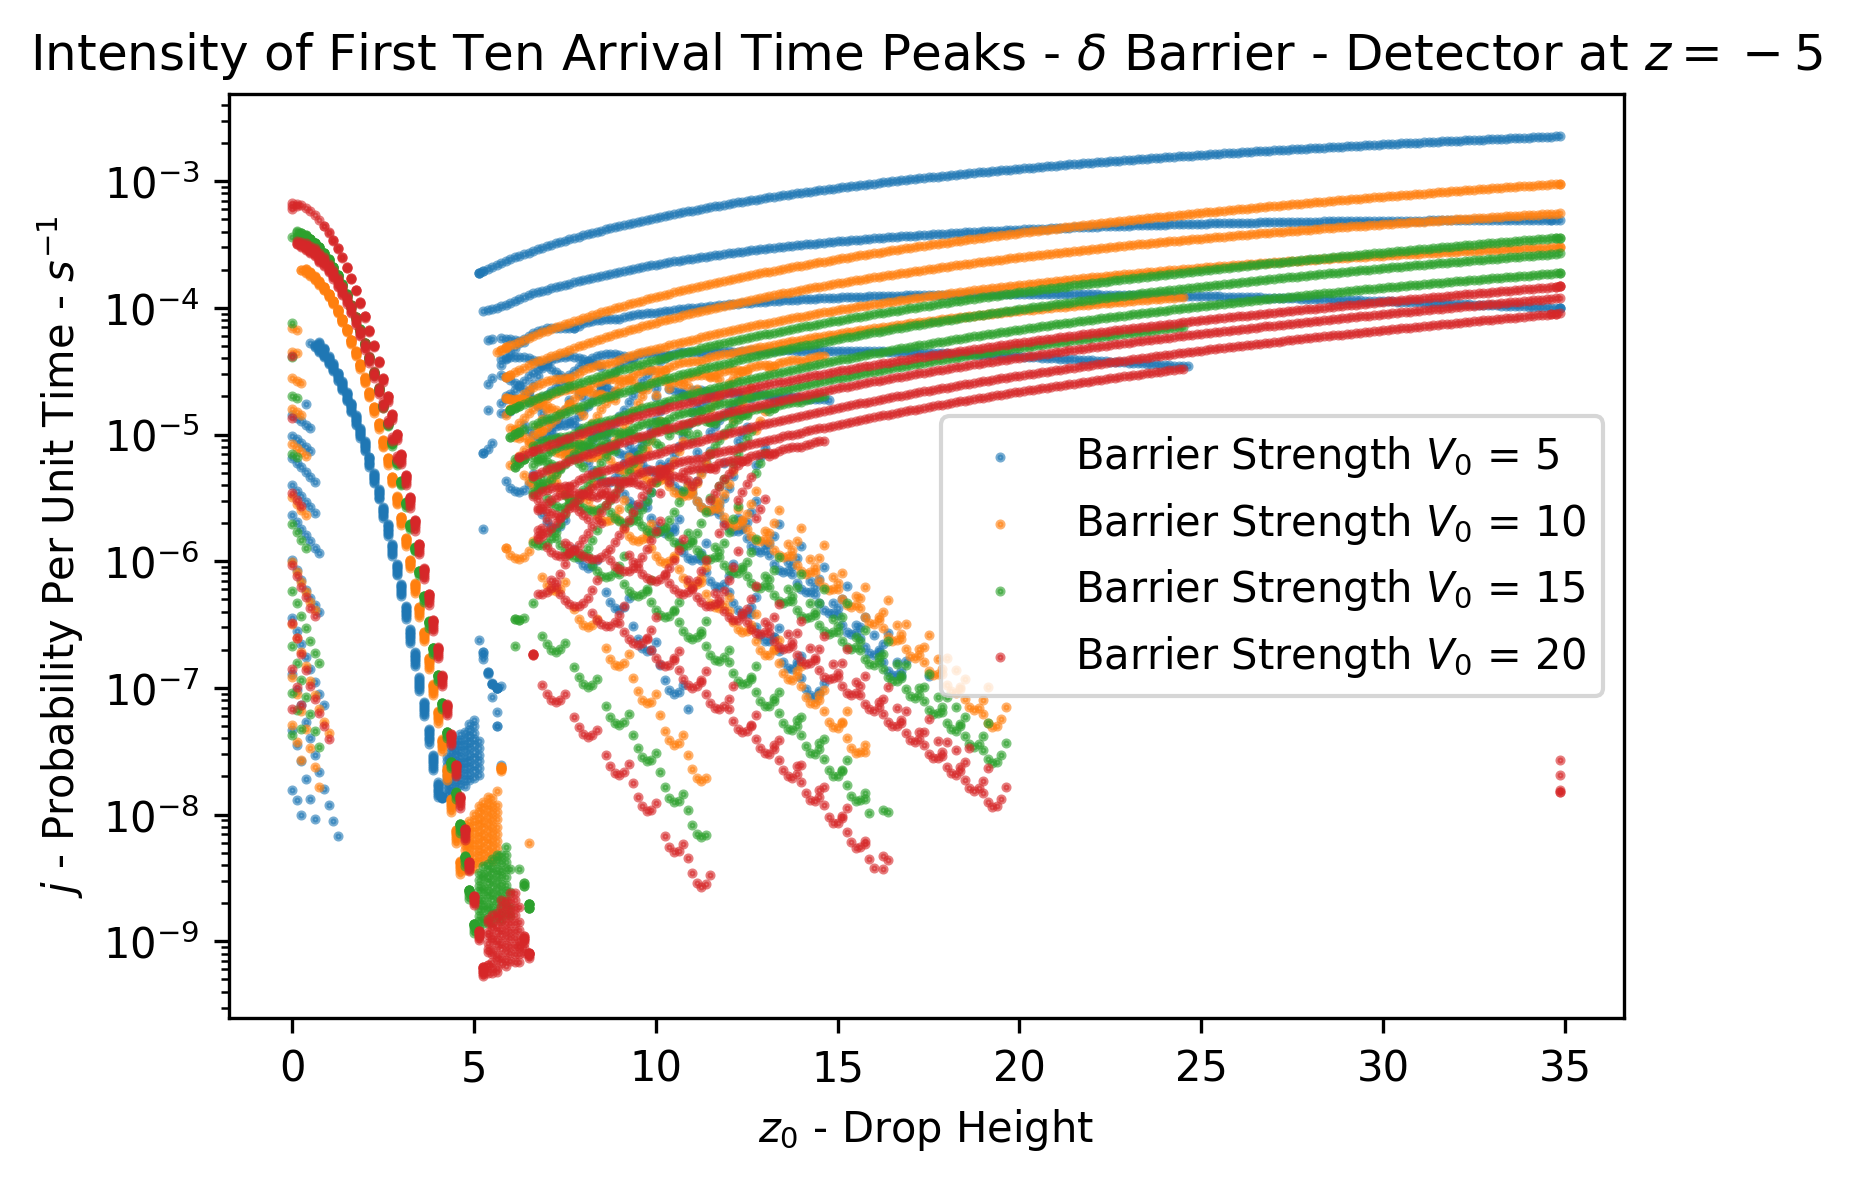
\includegraphics[width=1\linewidth]{Figures//Yoshida/f15d6e33-0b1f-4663-83da-2a213884a29c.png}
    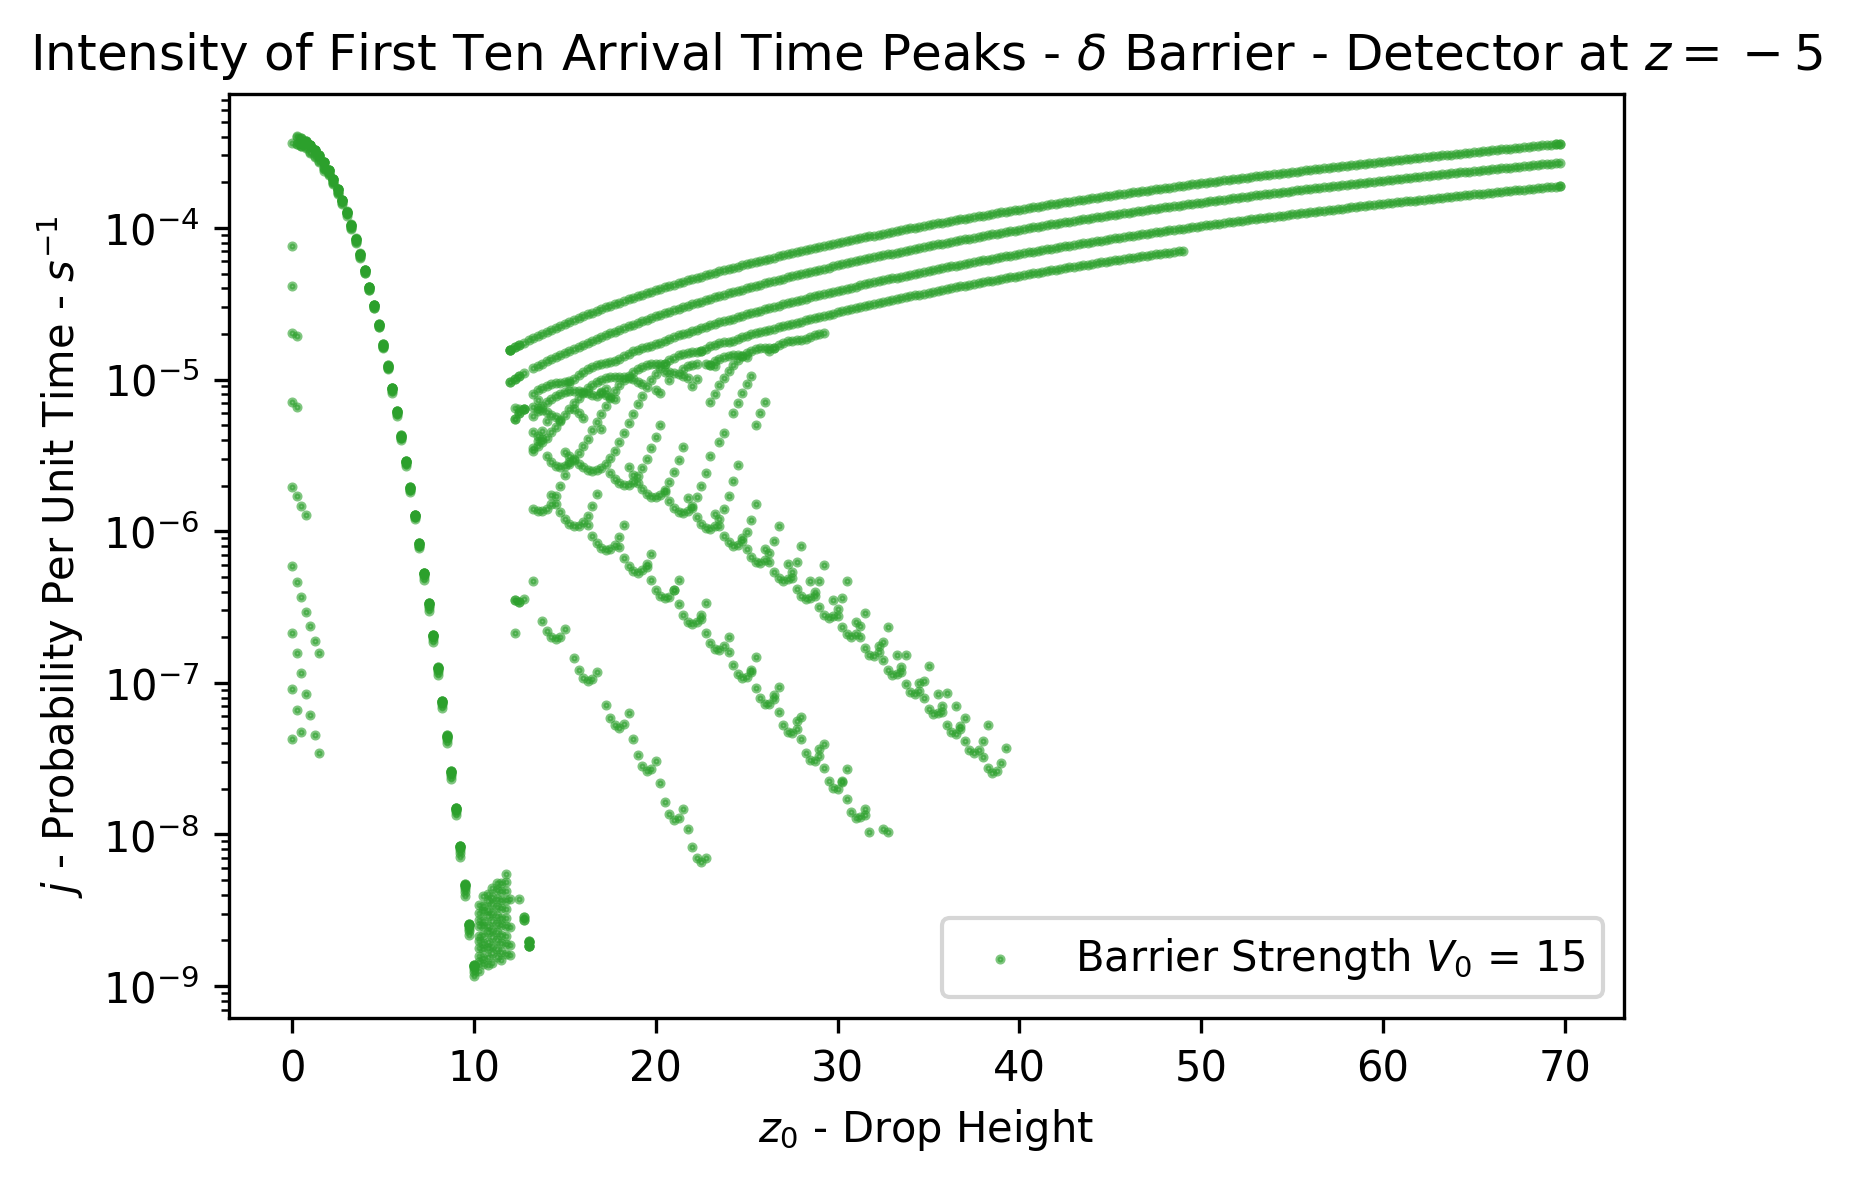
\includegraphics[width=1\linewidth]{Figures//Yoshida/91e57465-286b-4d77-8f46-f8cee493fd29.png}
    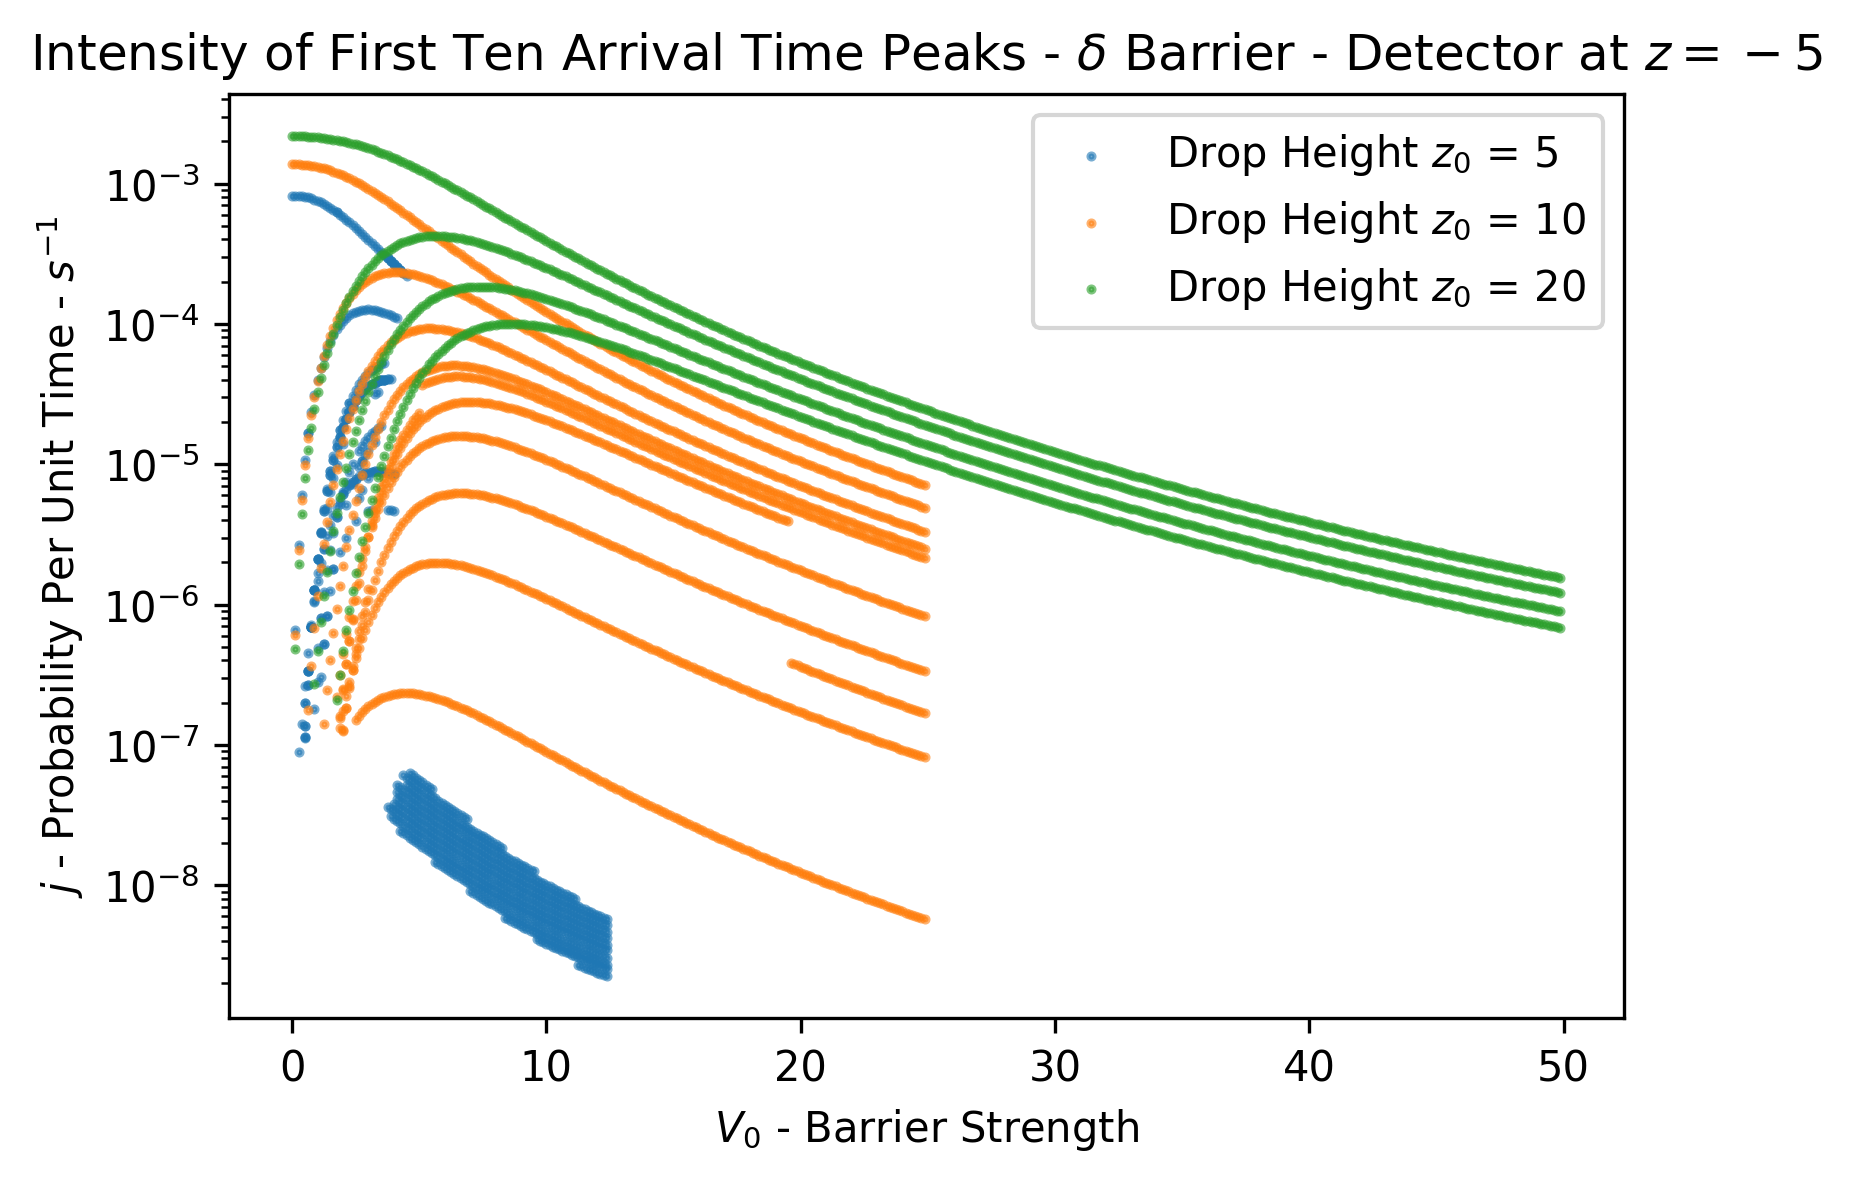
\includegraphics[width=1\linewidth]{Figures//Yoshida/d6c62d40-afdb-4fae-ae27-7c2a728c4b16.png}
    
    \caption{Peaks in Arrival Time \textbf{(Intensity)} Distribution for a Delta barrier. Notice the regularity of arrival intensities above 5 drop units in the upper chart making the delta barrier seem to approximate to semi-classical predictions which need further theoretical considerations. On the lower graph, it's clearly seen that regardless of barrier strength, the four situations produce the same peak distribution in seconds, except for the transitionary region at 5 units in drop height.}
    \label{fig:delta_intensity_gazon}
\end{figure}

% gamma simulations 1028
\begin{figure}
    \centering
    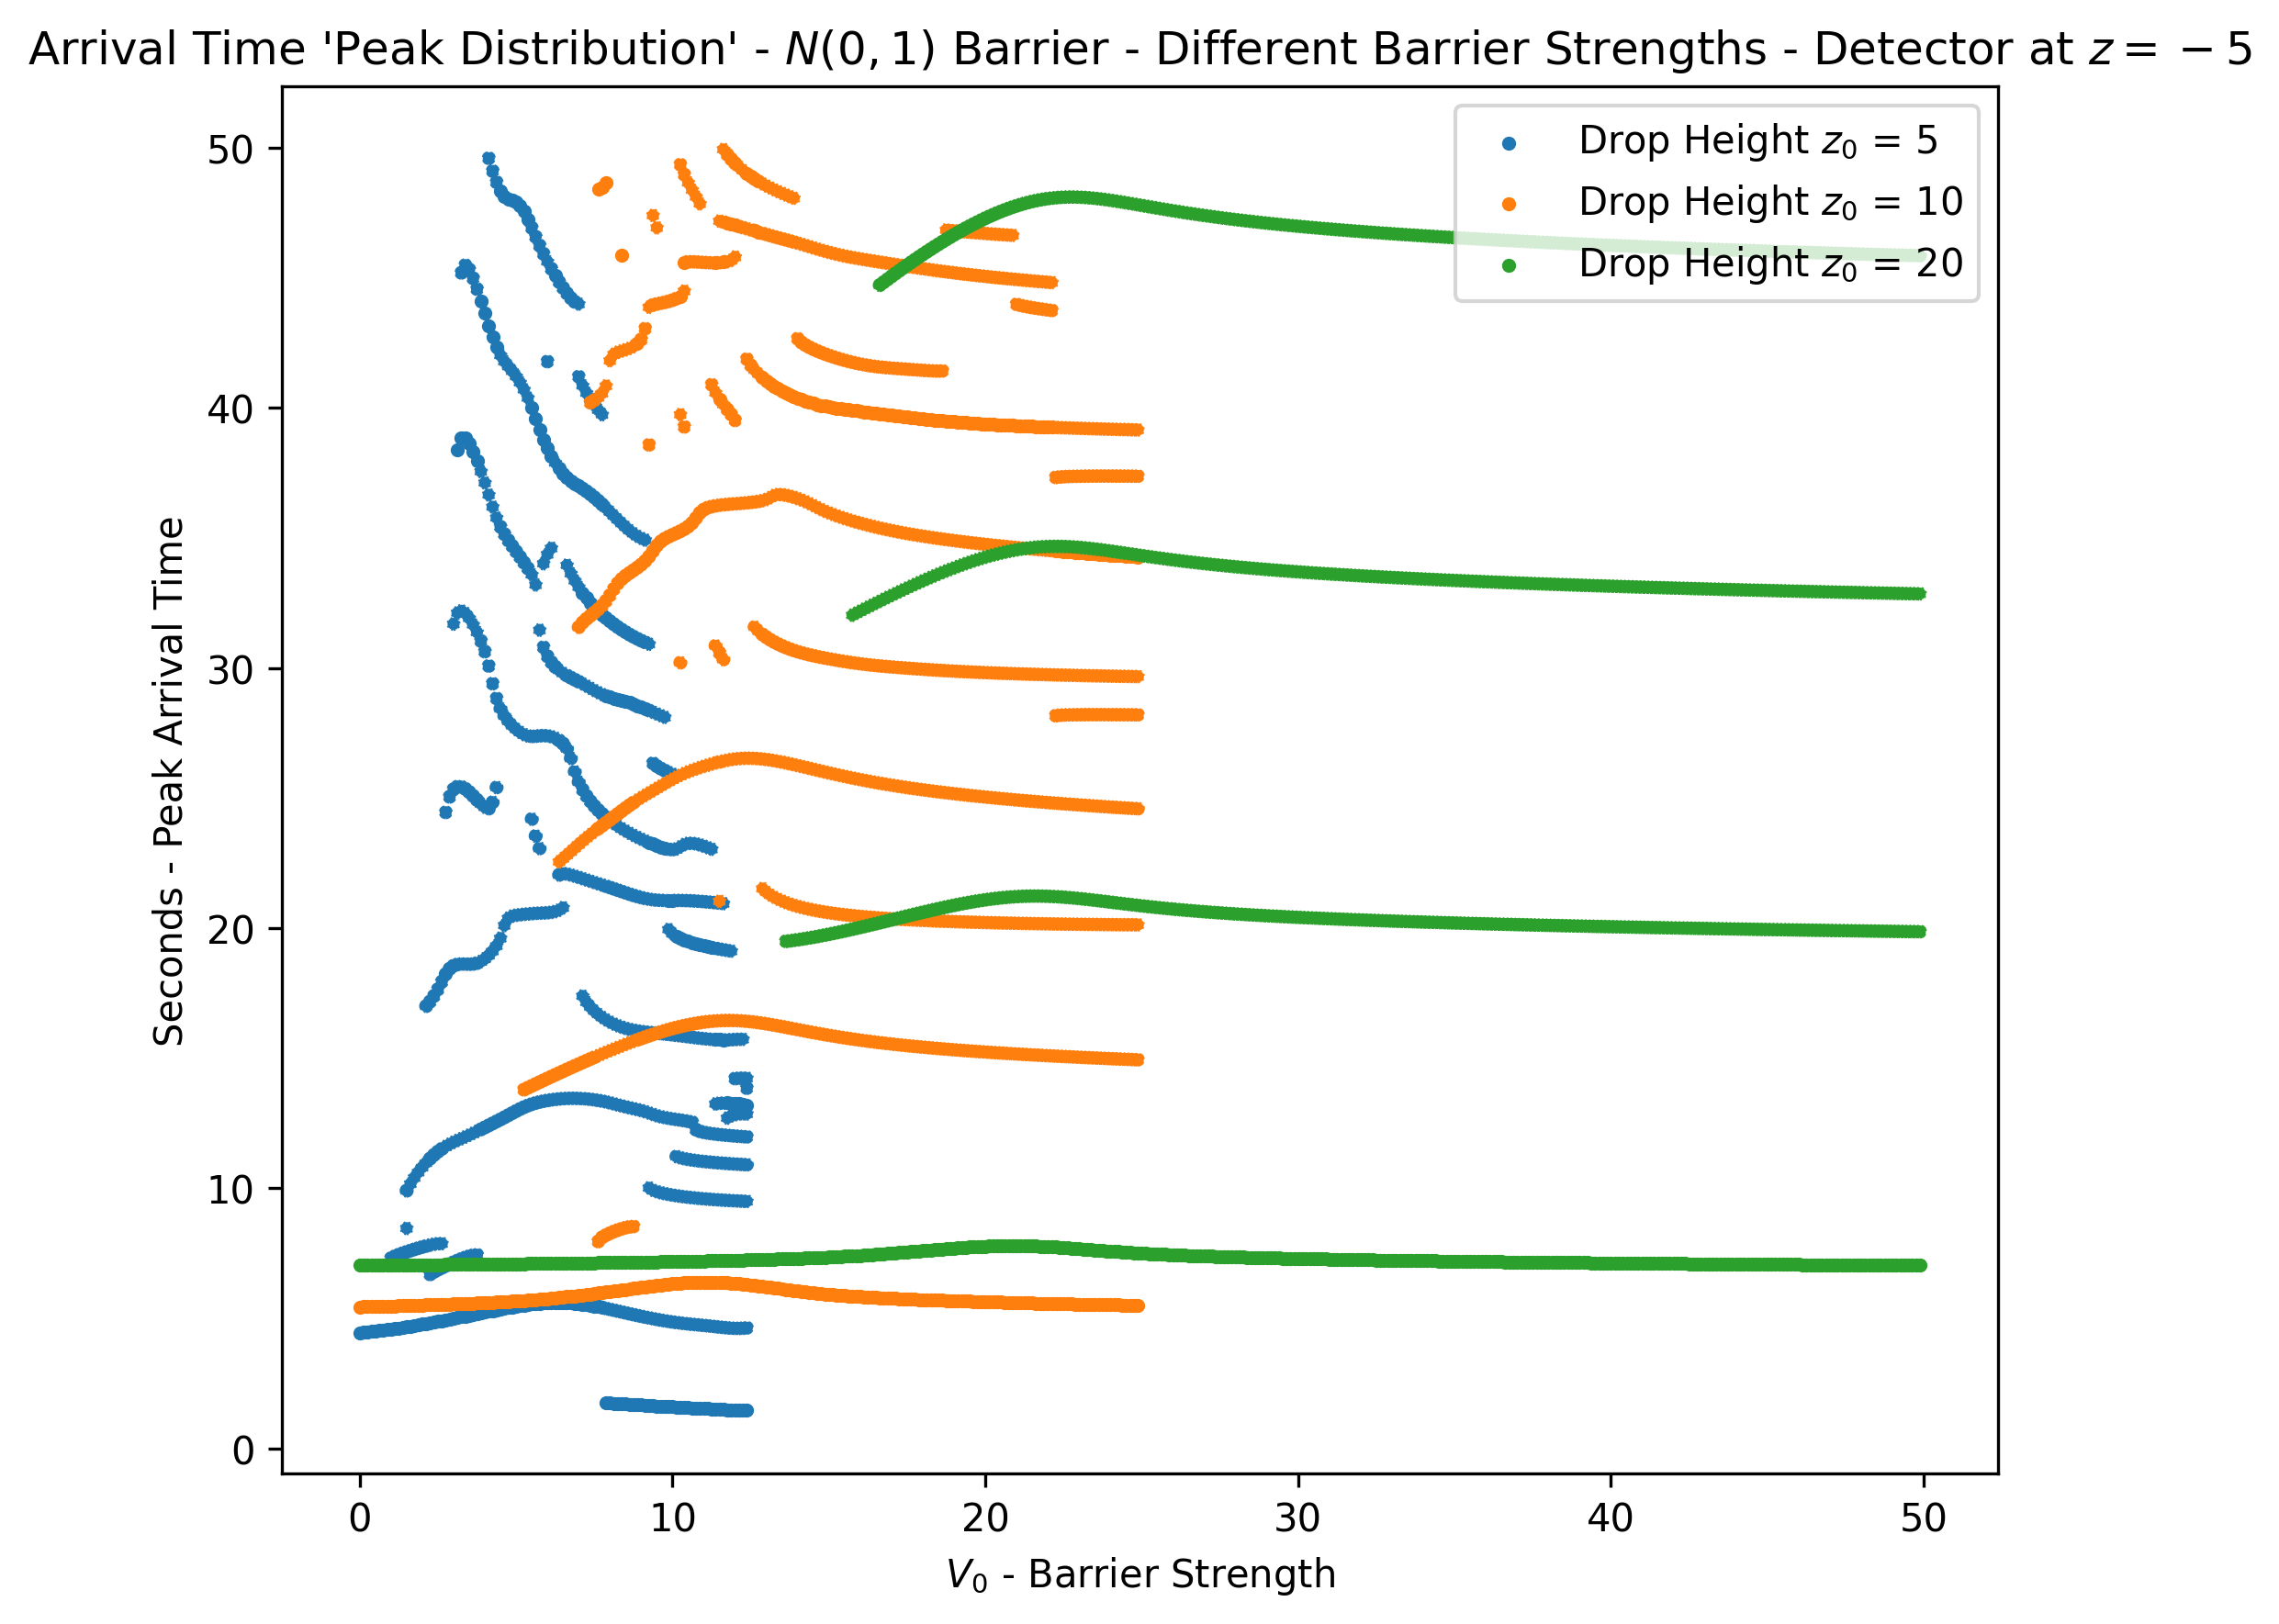
\includegraphics[width=1\linewidth]{Figures//Yoshida/3444d7de-b27d-4a56-9831-5486c5e74929.png}
    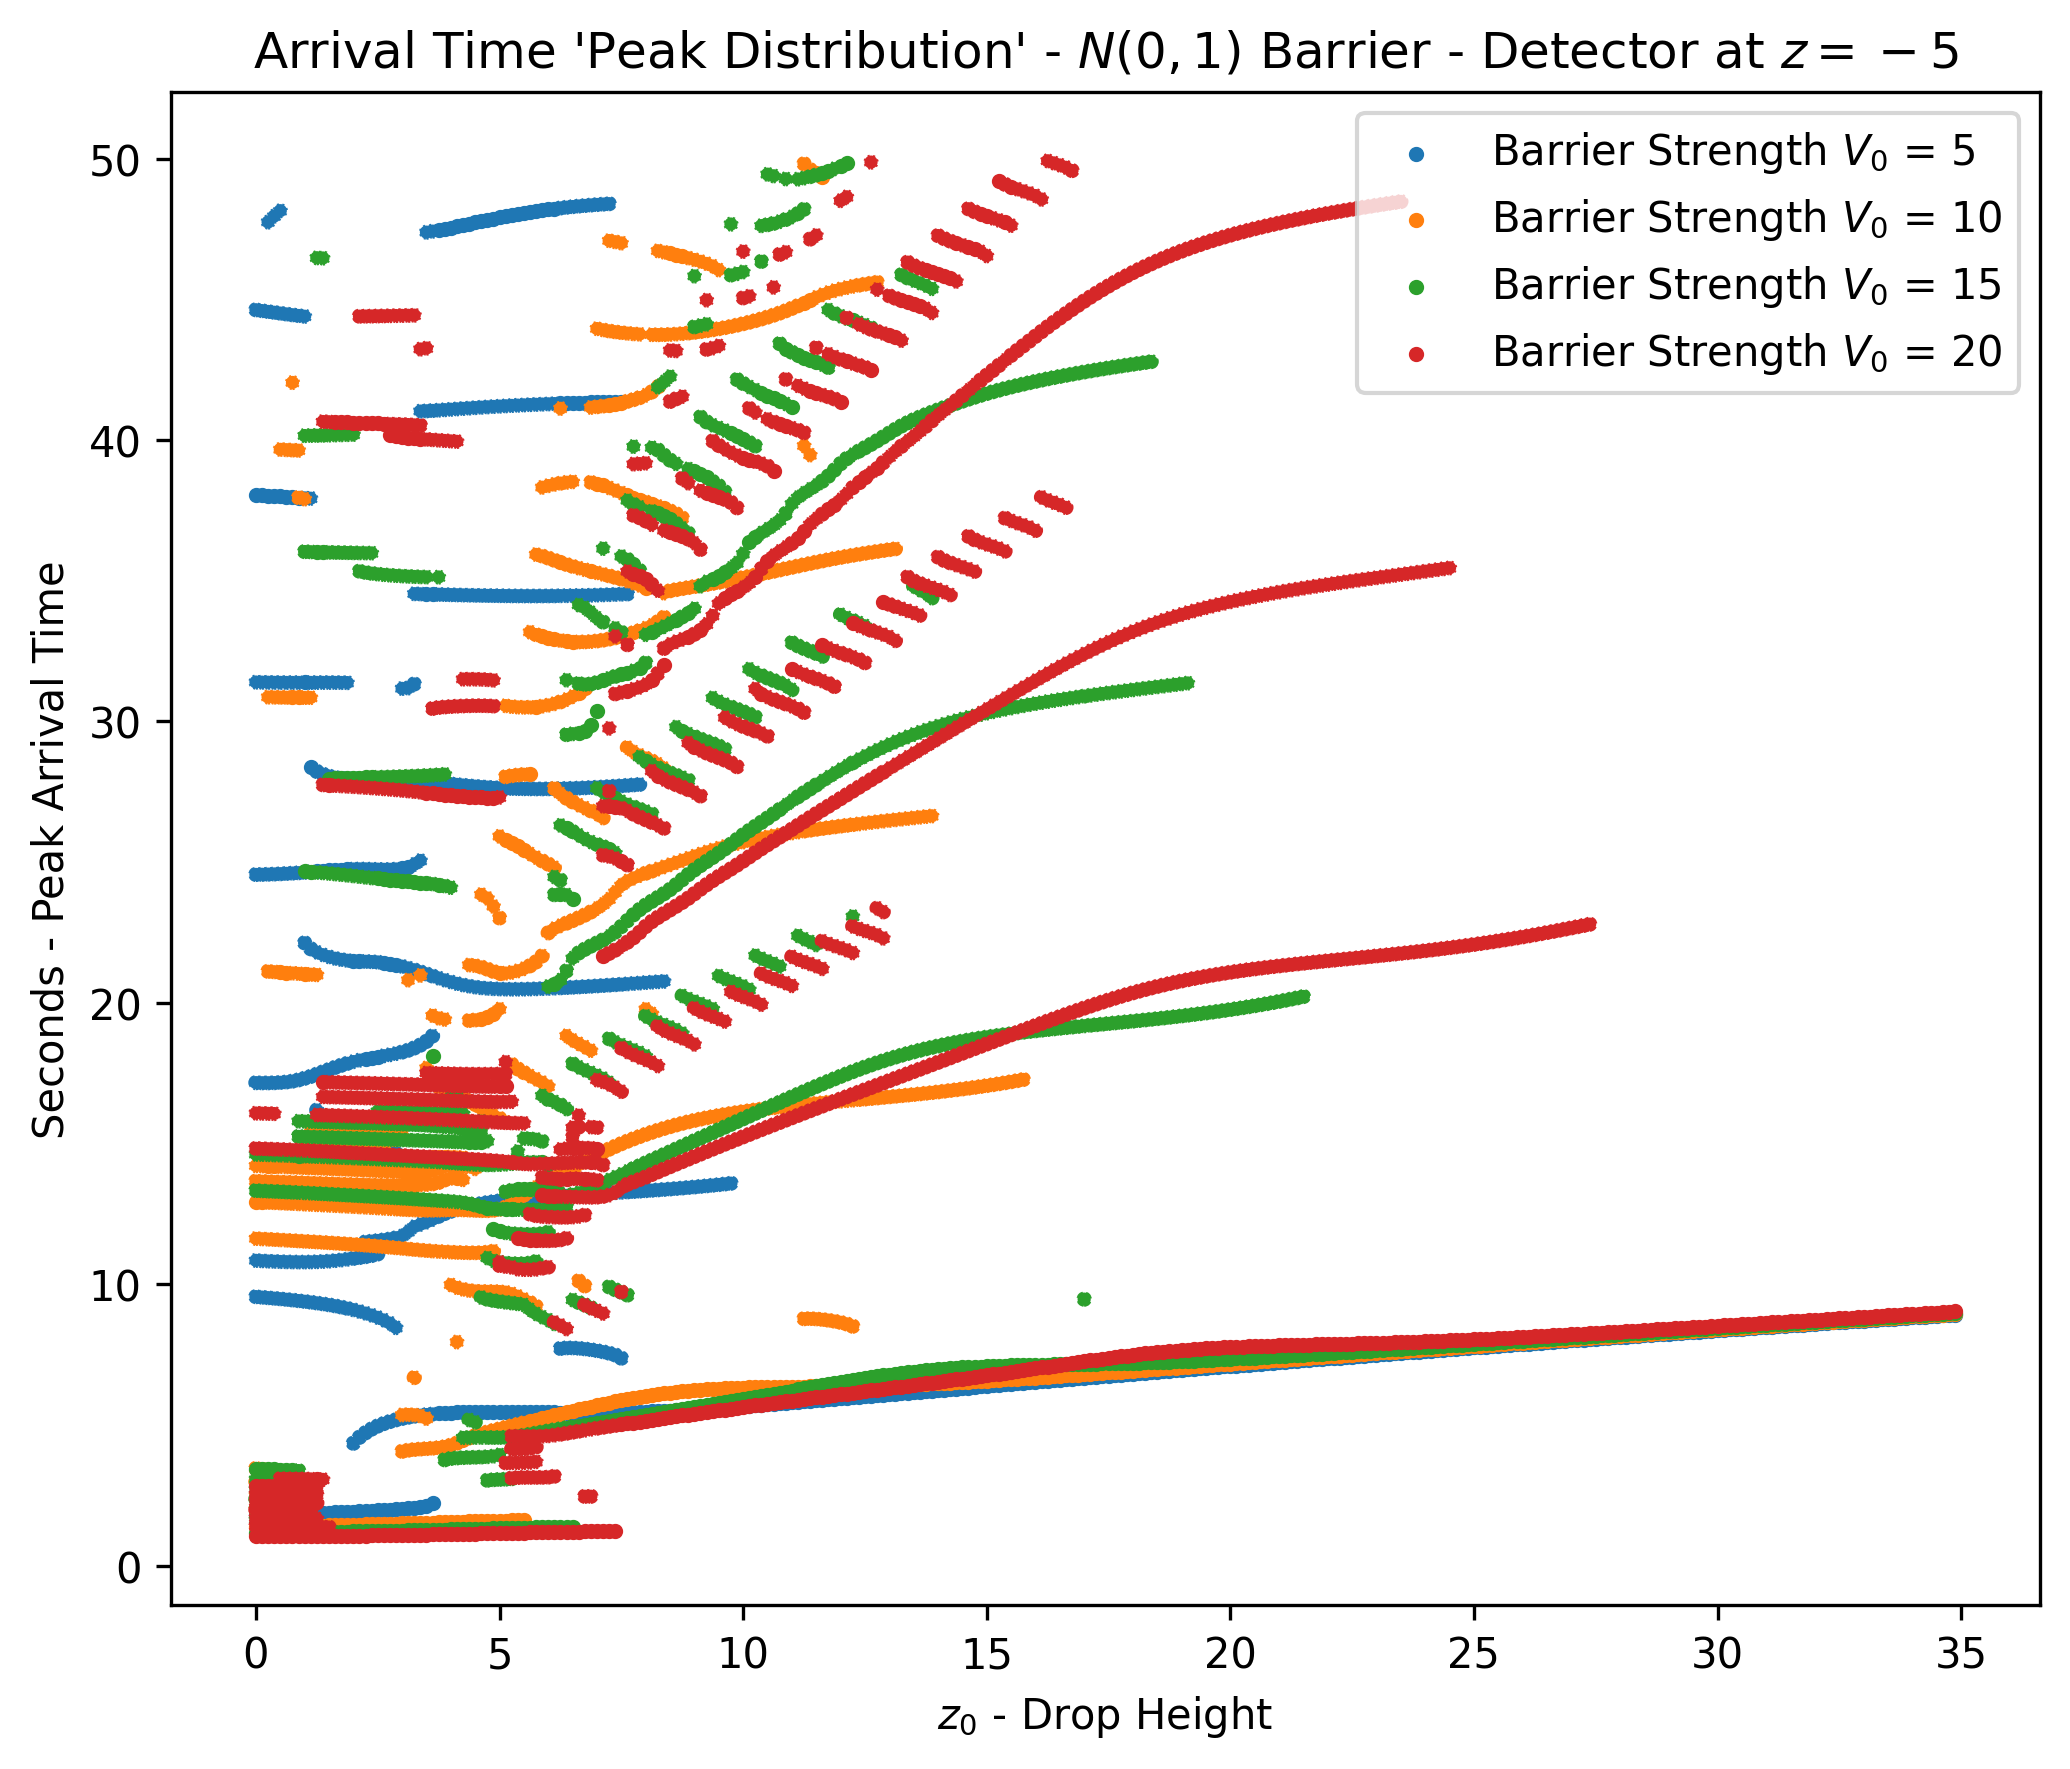
\includegraphics[width=1\linewidth]{Figures//Yoshida/0479695a-5c09-4aff-ba5e-298419ff081f.png}
    \caption{Peaks in Arrival Time \textbf{(seconds)} Distribution for a Gaussian barrier. Notice the highly non-trivial of arrival times above 5 drop units. There are, however, discernable features to be recognized. The upper figure features band-formation in the (10,42) region, and show cases tunnelling resonances when observing the peaks of the green arrival times: semi-stable standing waves seems to be created at adequate energies (drop heights) causing the particle to arrive later than anticpated. Upon subsequent reflections, the particle loses energy in a non-linear way, which contributes to the non-linear arrival time distribution. On the lower figure, it's of considerable interest to notice the clearly "continuous" arrival time, and the "broken" odd arrival time.}
    \label{fig:normalPEAKS_YO}
\end{figure}

\begin{figure}
    \centering
    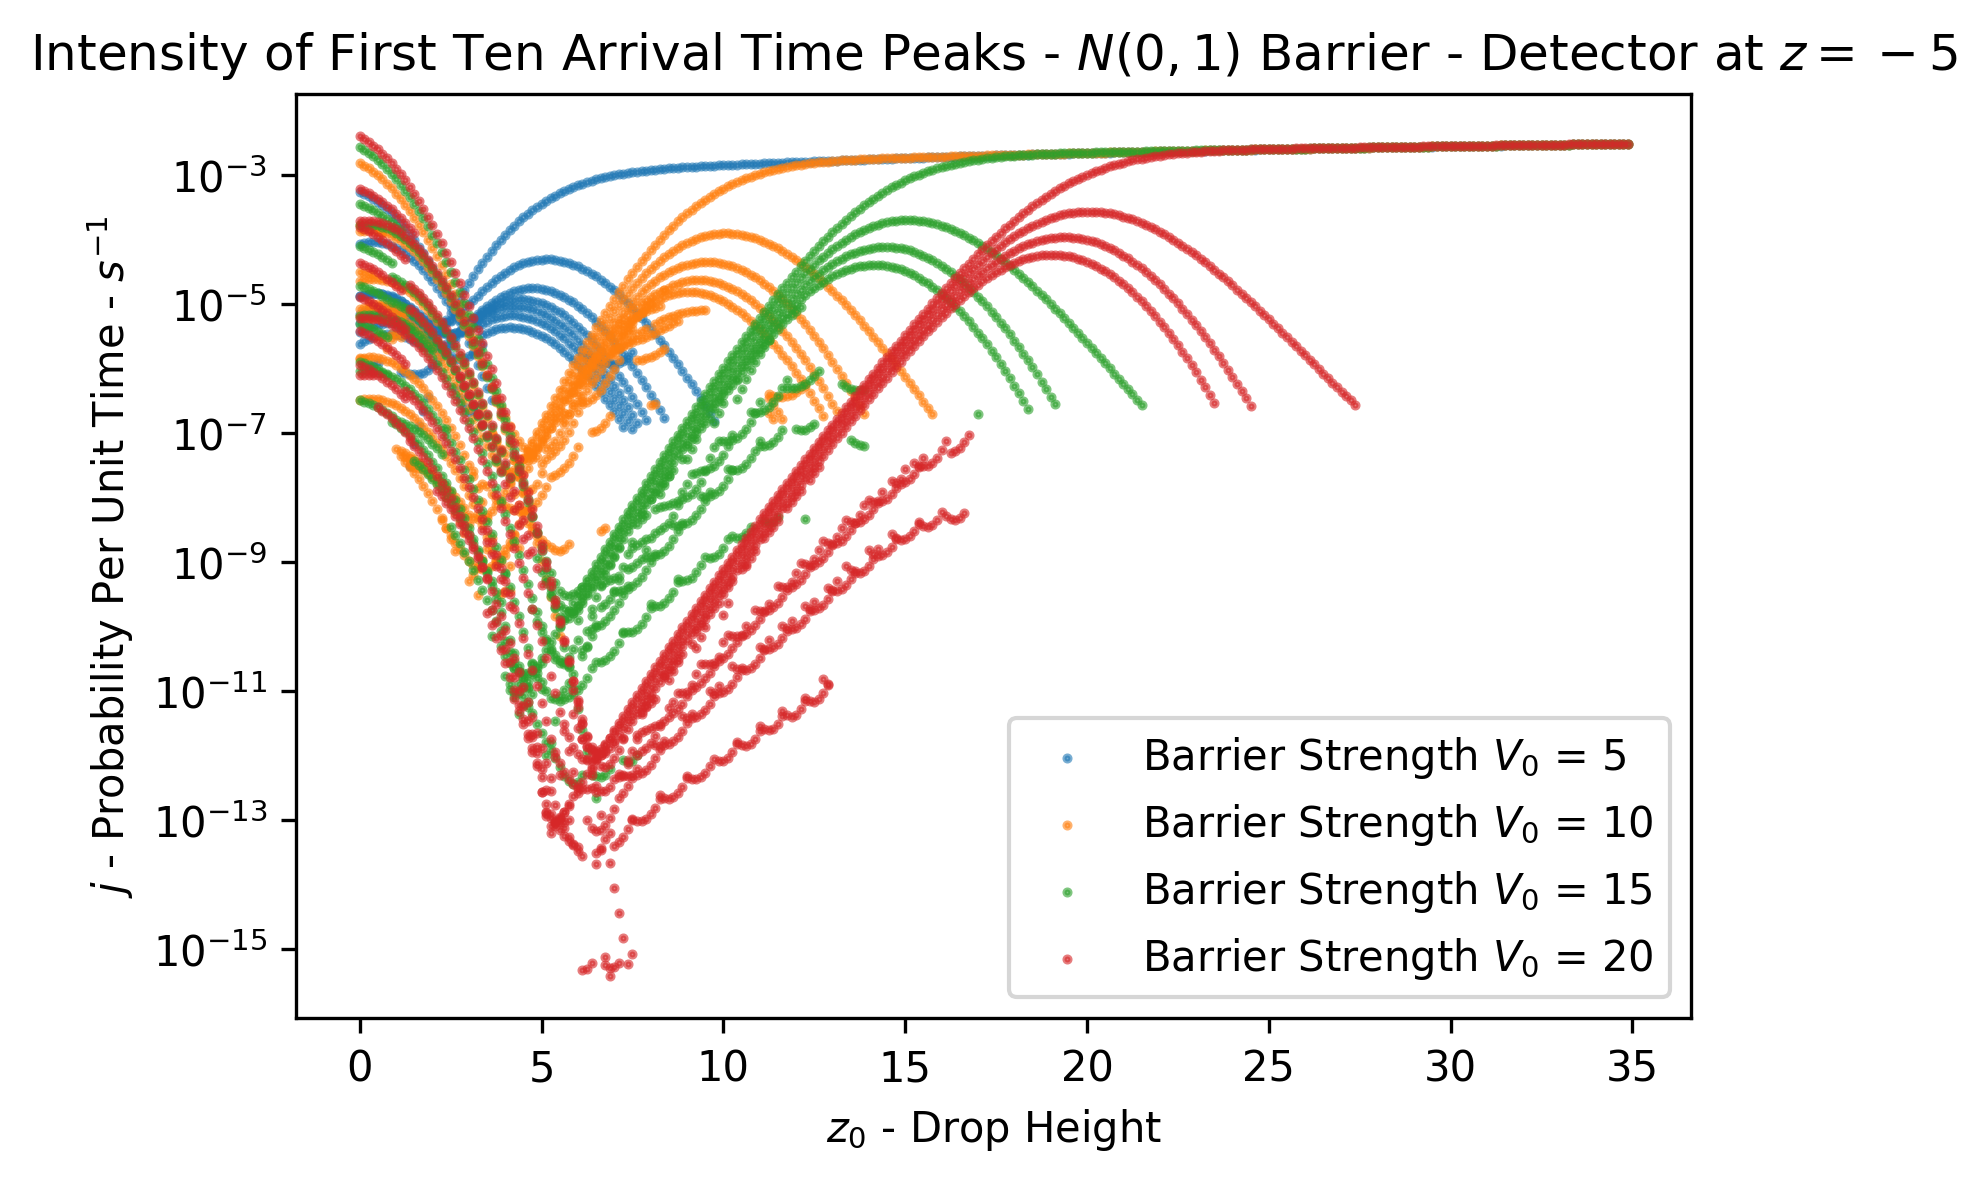
\includegraphics[width=1\linewidth]{Figures//Yoshida/89407939-0f3f-4362-b47d-f2ebf2cfd959.png}
    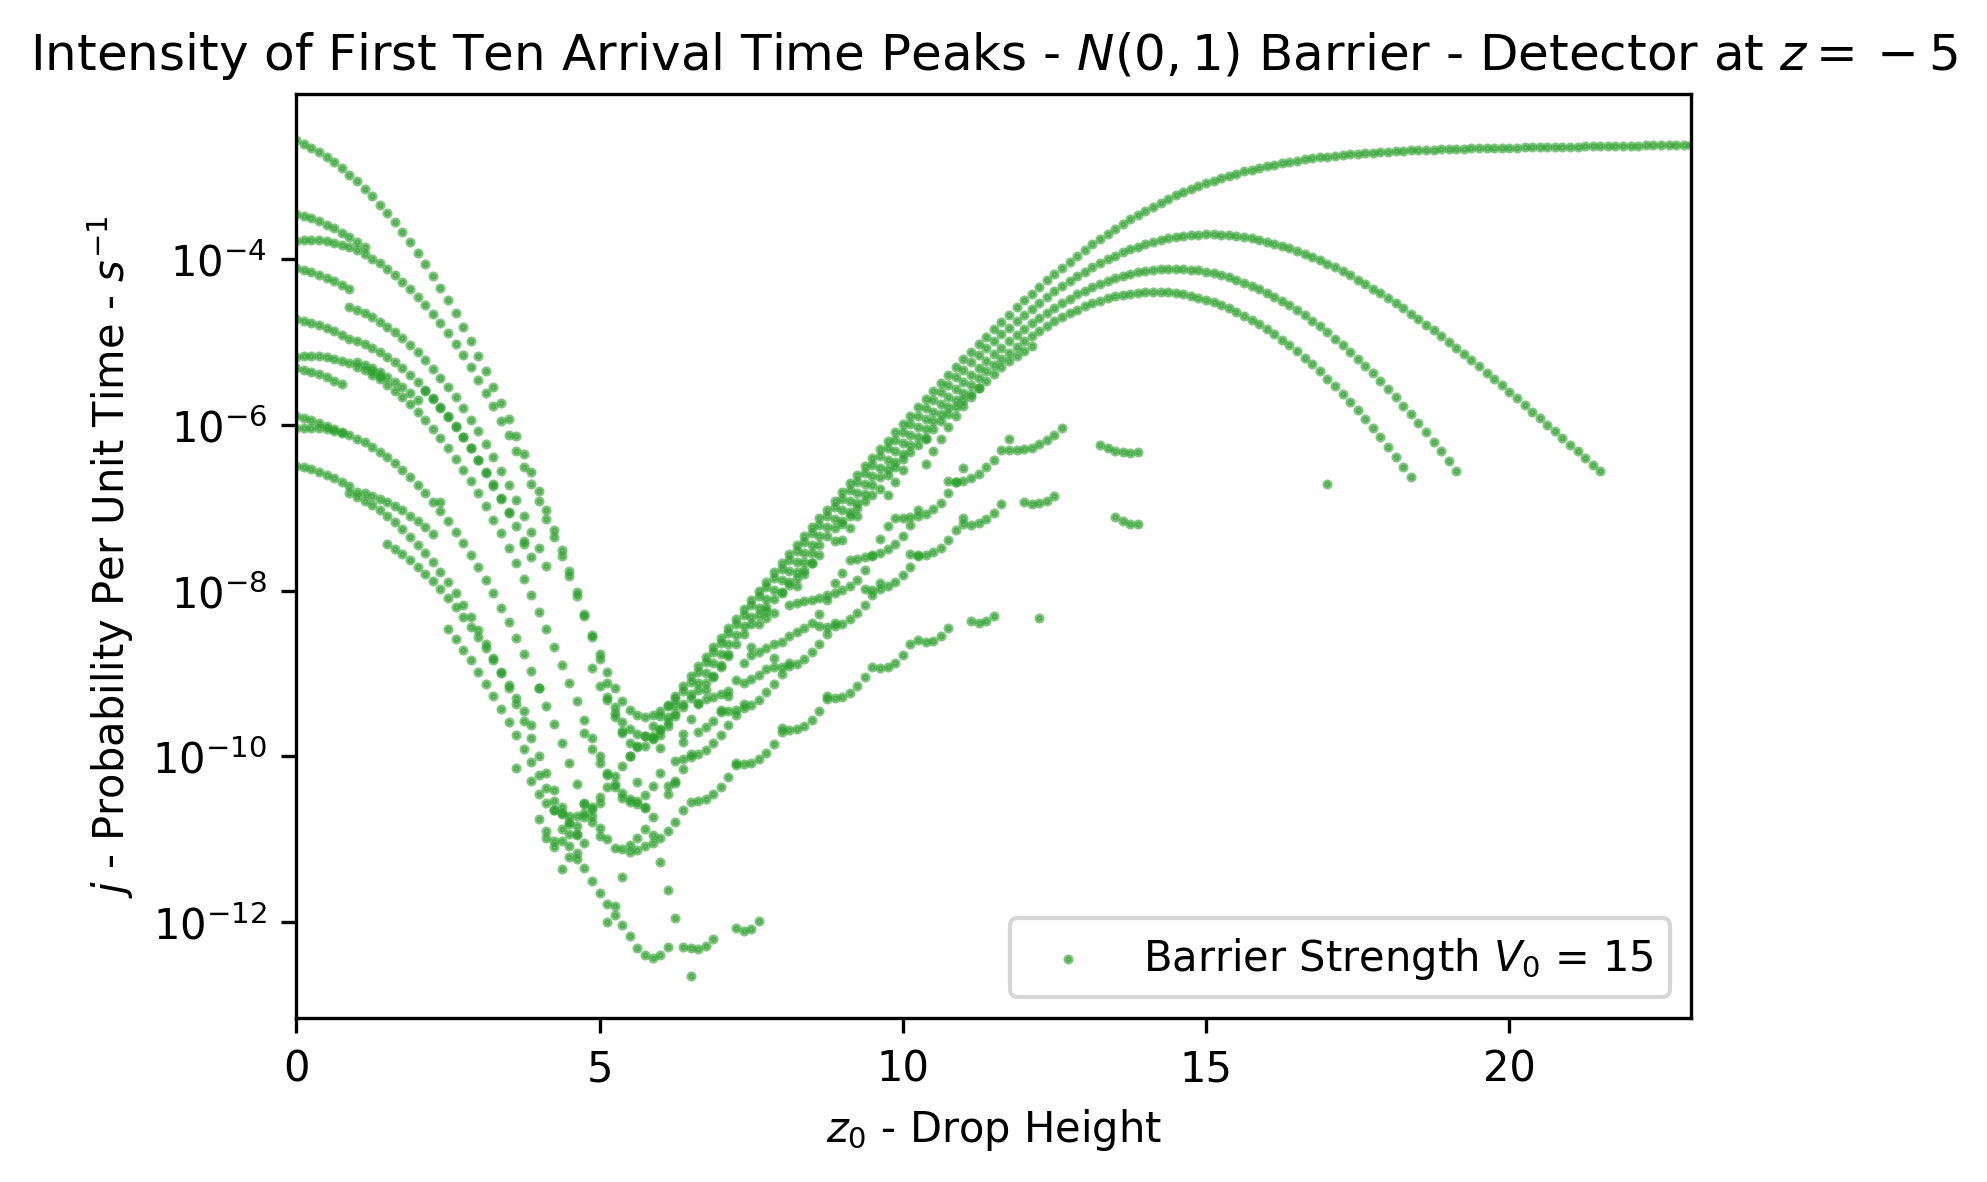
\includegraphics[width=1\linewidth]{Figures//Yoshida/4606fc0c-a23b-47dc-ae64-2a791fe3fd5b.png}
    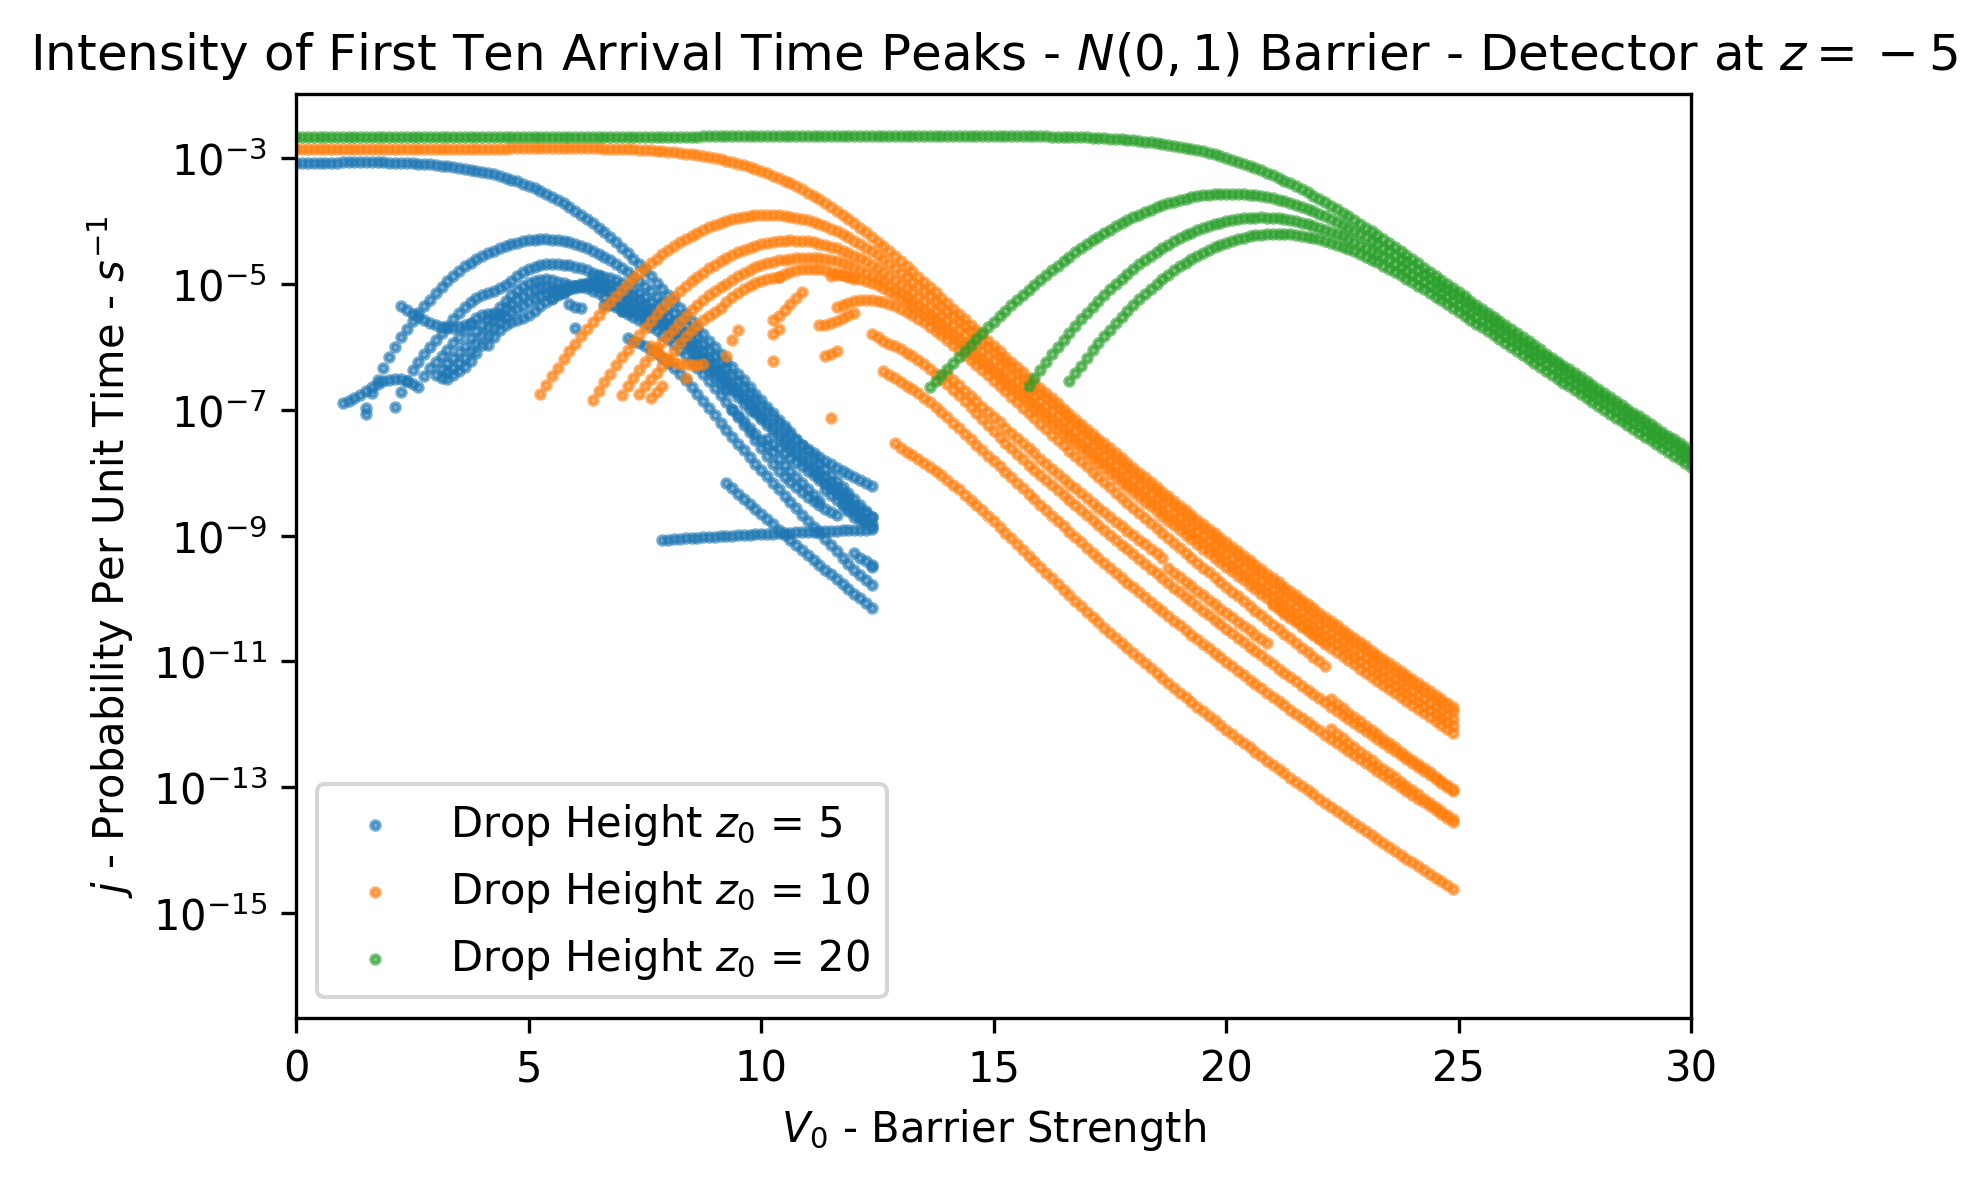
\includegraphics[width=1\linewidth]{Figures//Yoshida/e3ca365e-0e36-49bf-87a0-363c8a26e34f.png}
    
    \caption{Peaks in Arrival Time \textbf{(Intensity)} Distribution for a Gaussian barrier, in function of drop height and barrier strength. Interesting non-linear features can be observed. What's noticable is the parabola-like formation of the intensity curves of the non-first arrival times, while asymptotically coming closer to one other for higher barrier strengths. On the upper graph, all arrival intensities seem to coincide before they spread, which could be properly characterized and treated theoretically.}
    \label{fig:yo-this-is-cool}
\end{figure}

% fitomg - second order channels
\begin{figure}
    \centering
    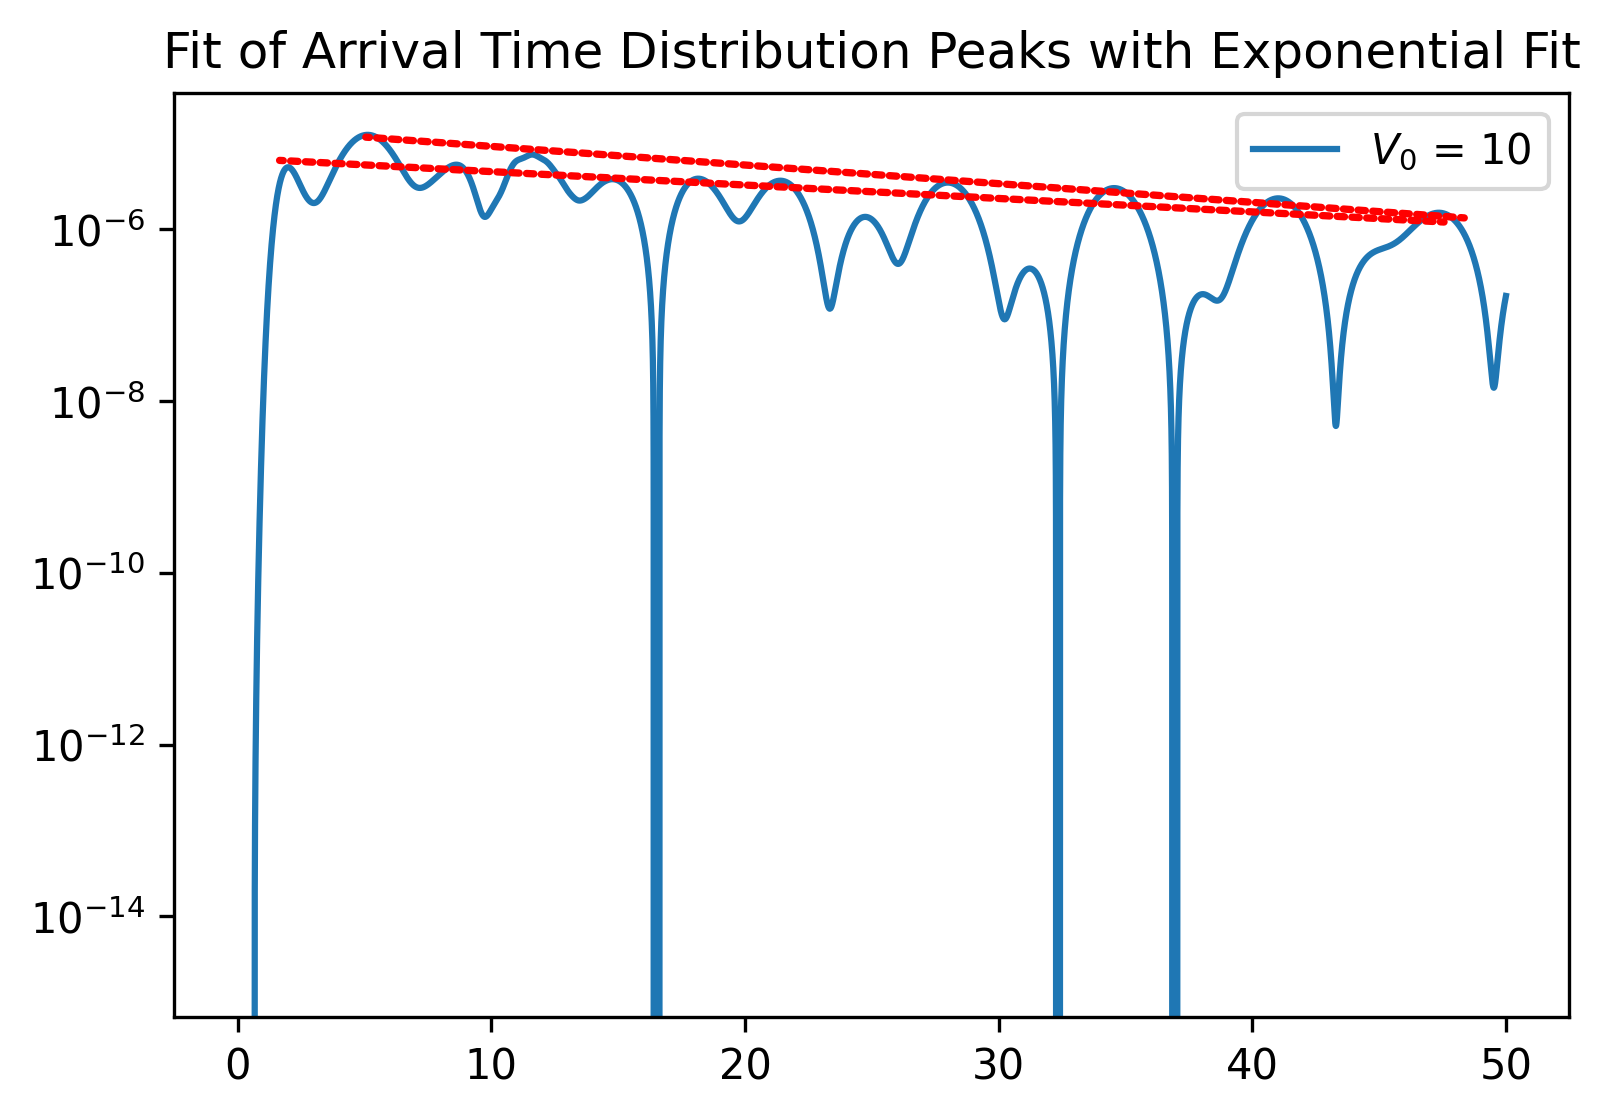
\includegraphics[width=1\linewidth]{Figures//Yoshida/fittingomg.png}
    
    \caption{Multiple Characterization possibilities when fitting arrival time peaks. Using a normal scipy.peaks function, all peaks would be identified, not distiquishing those "coming up from below" (primary reflections), and those who are "on top" (secondary reflections and quasi-stable wave formation in the barrier). Further work needs to be conducted.}
    \label{fig:fitomg}
\end{figure}

% Partile Drop Heights, Second Distributions
\begin{figure}
    \centering
    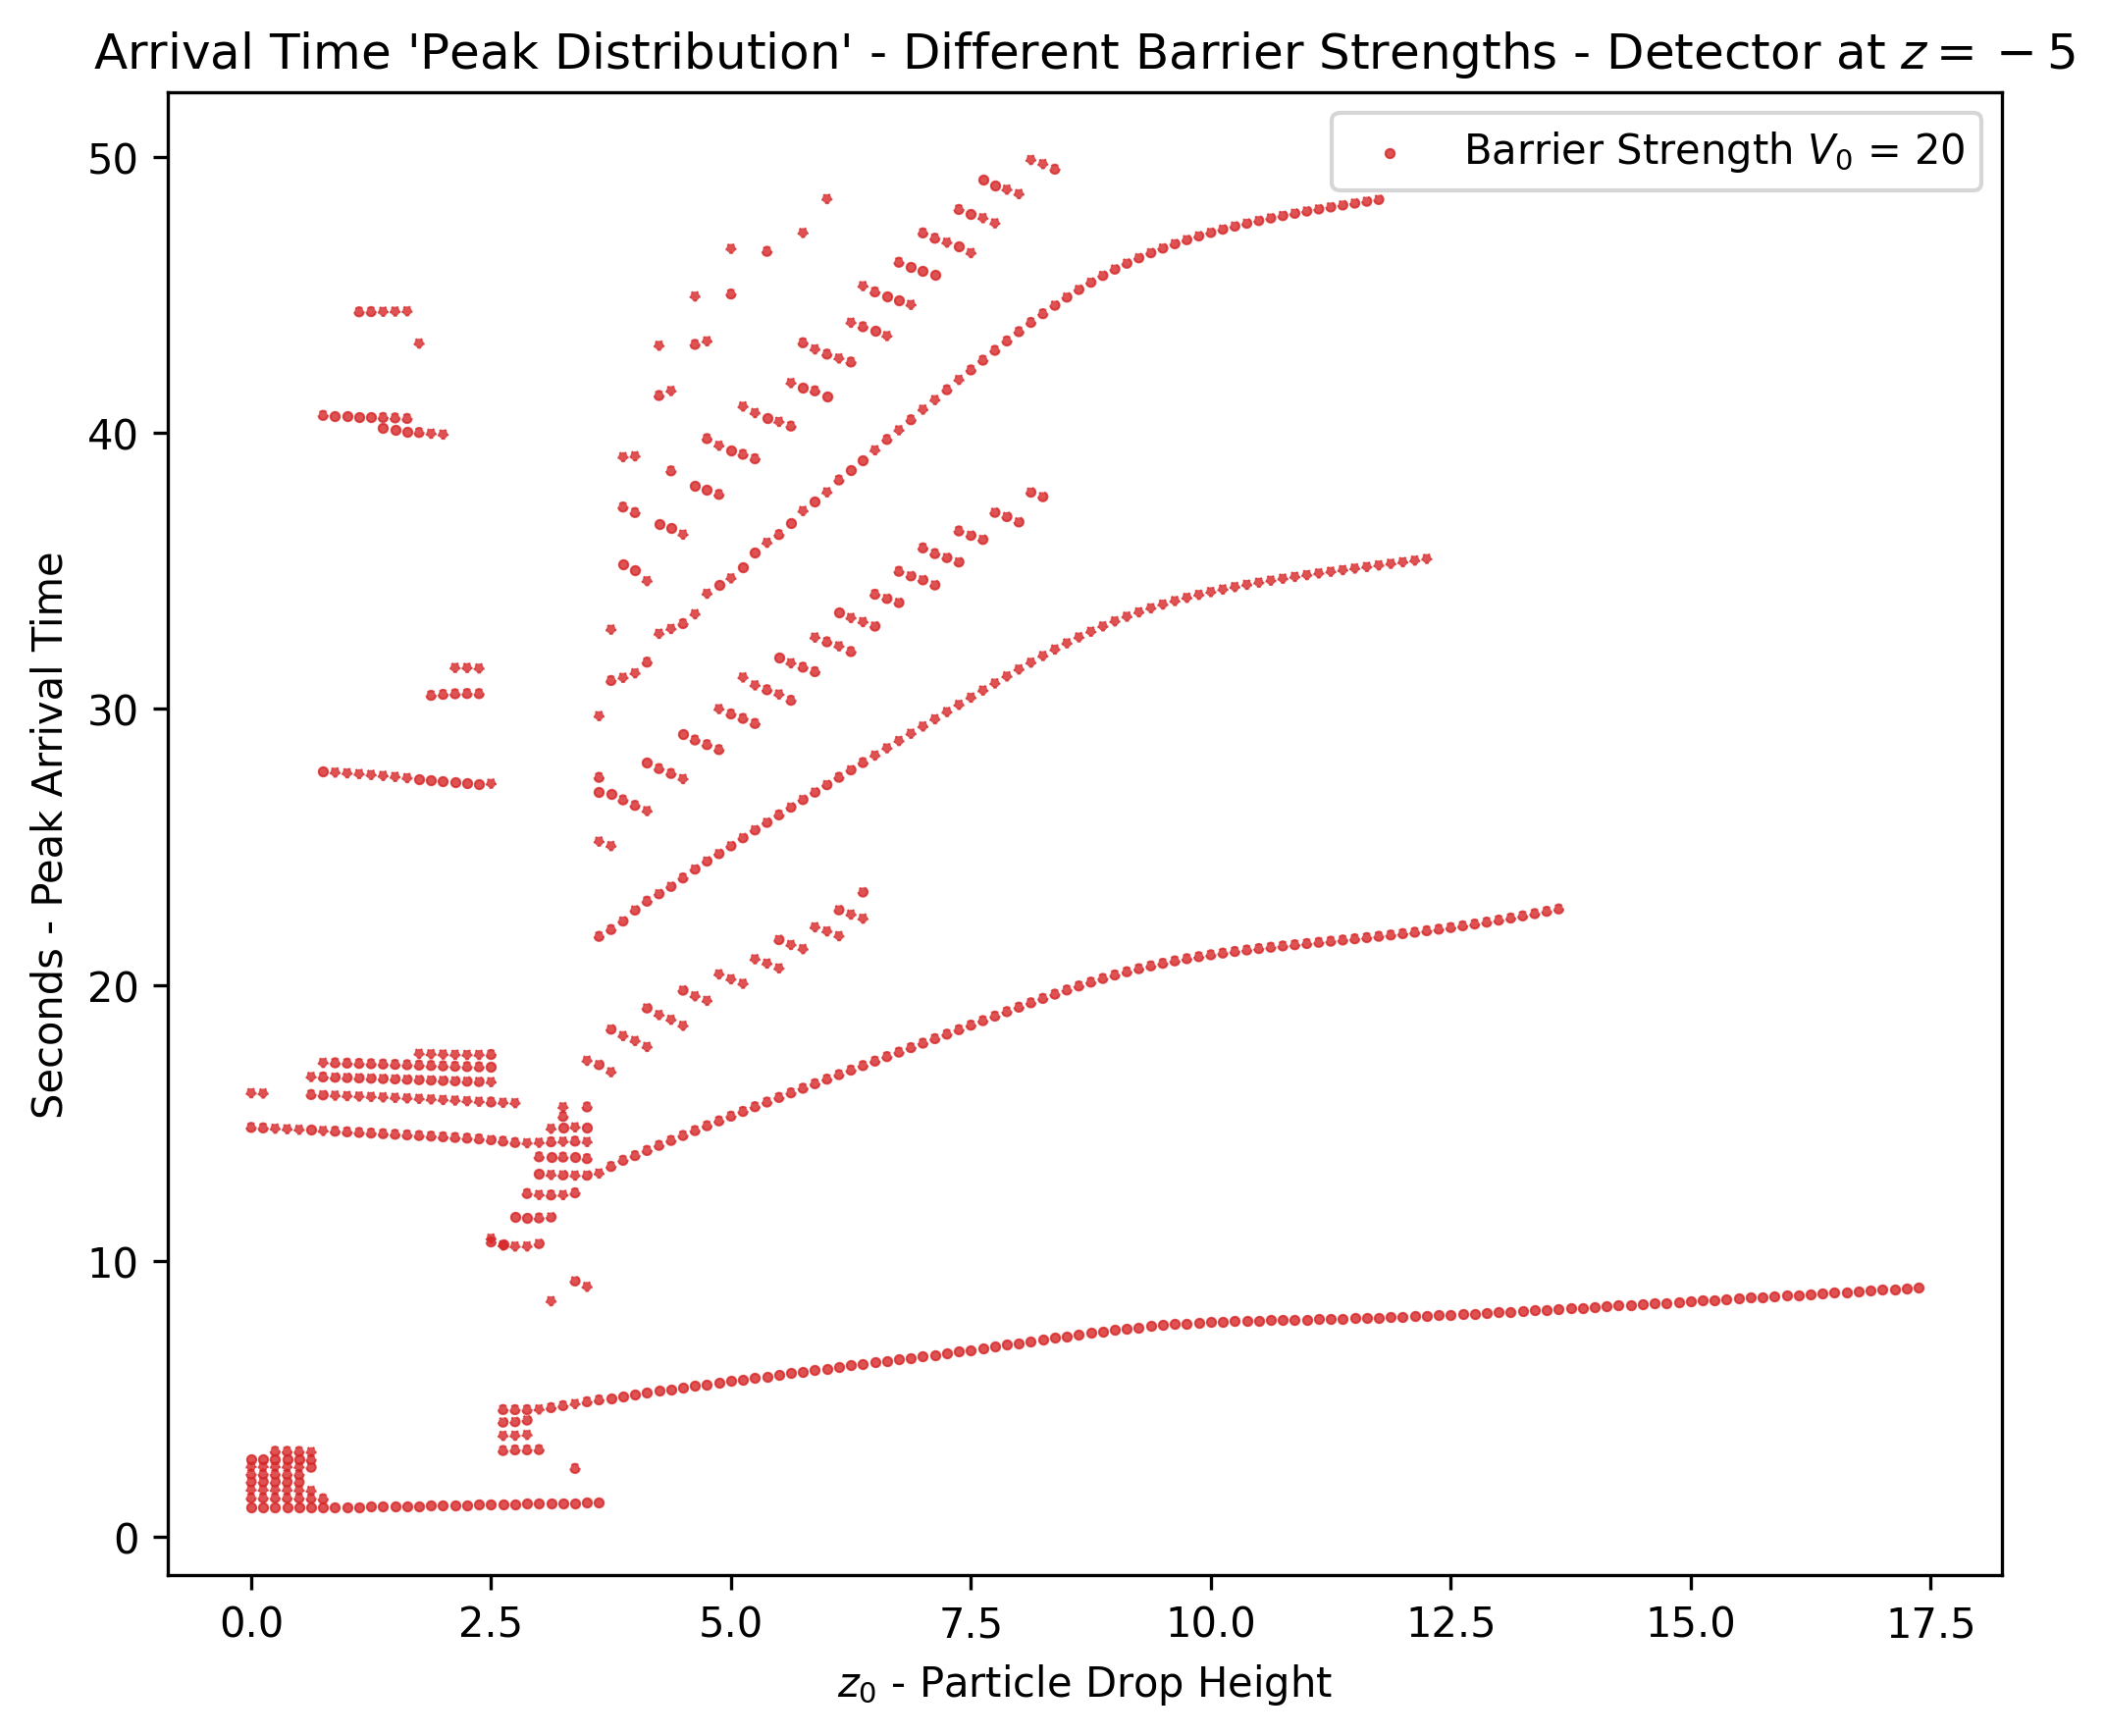
\includegraphics[width=1\linewidth]{Figures//Yoshida/6f850d7f-24cd-4888-a108-cb347683a759.png}
    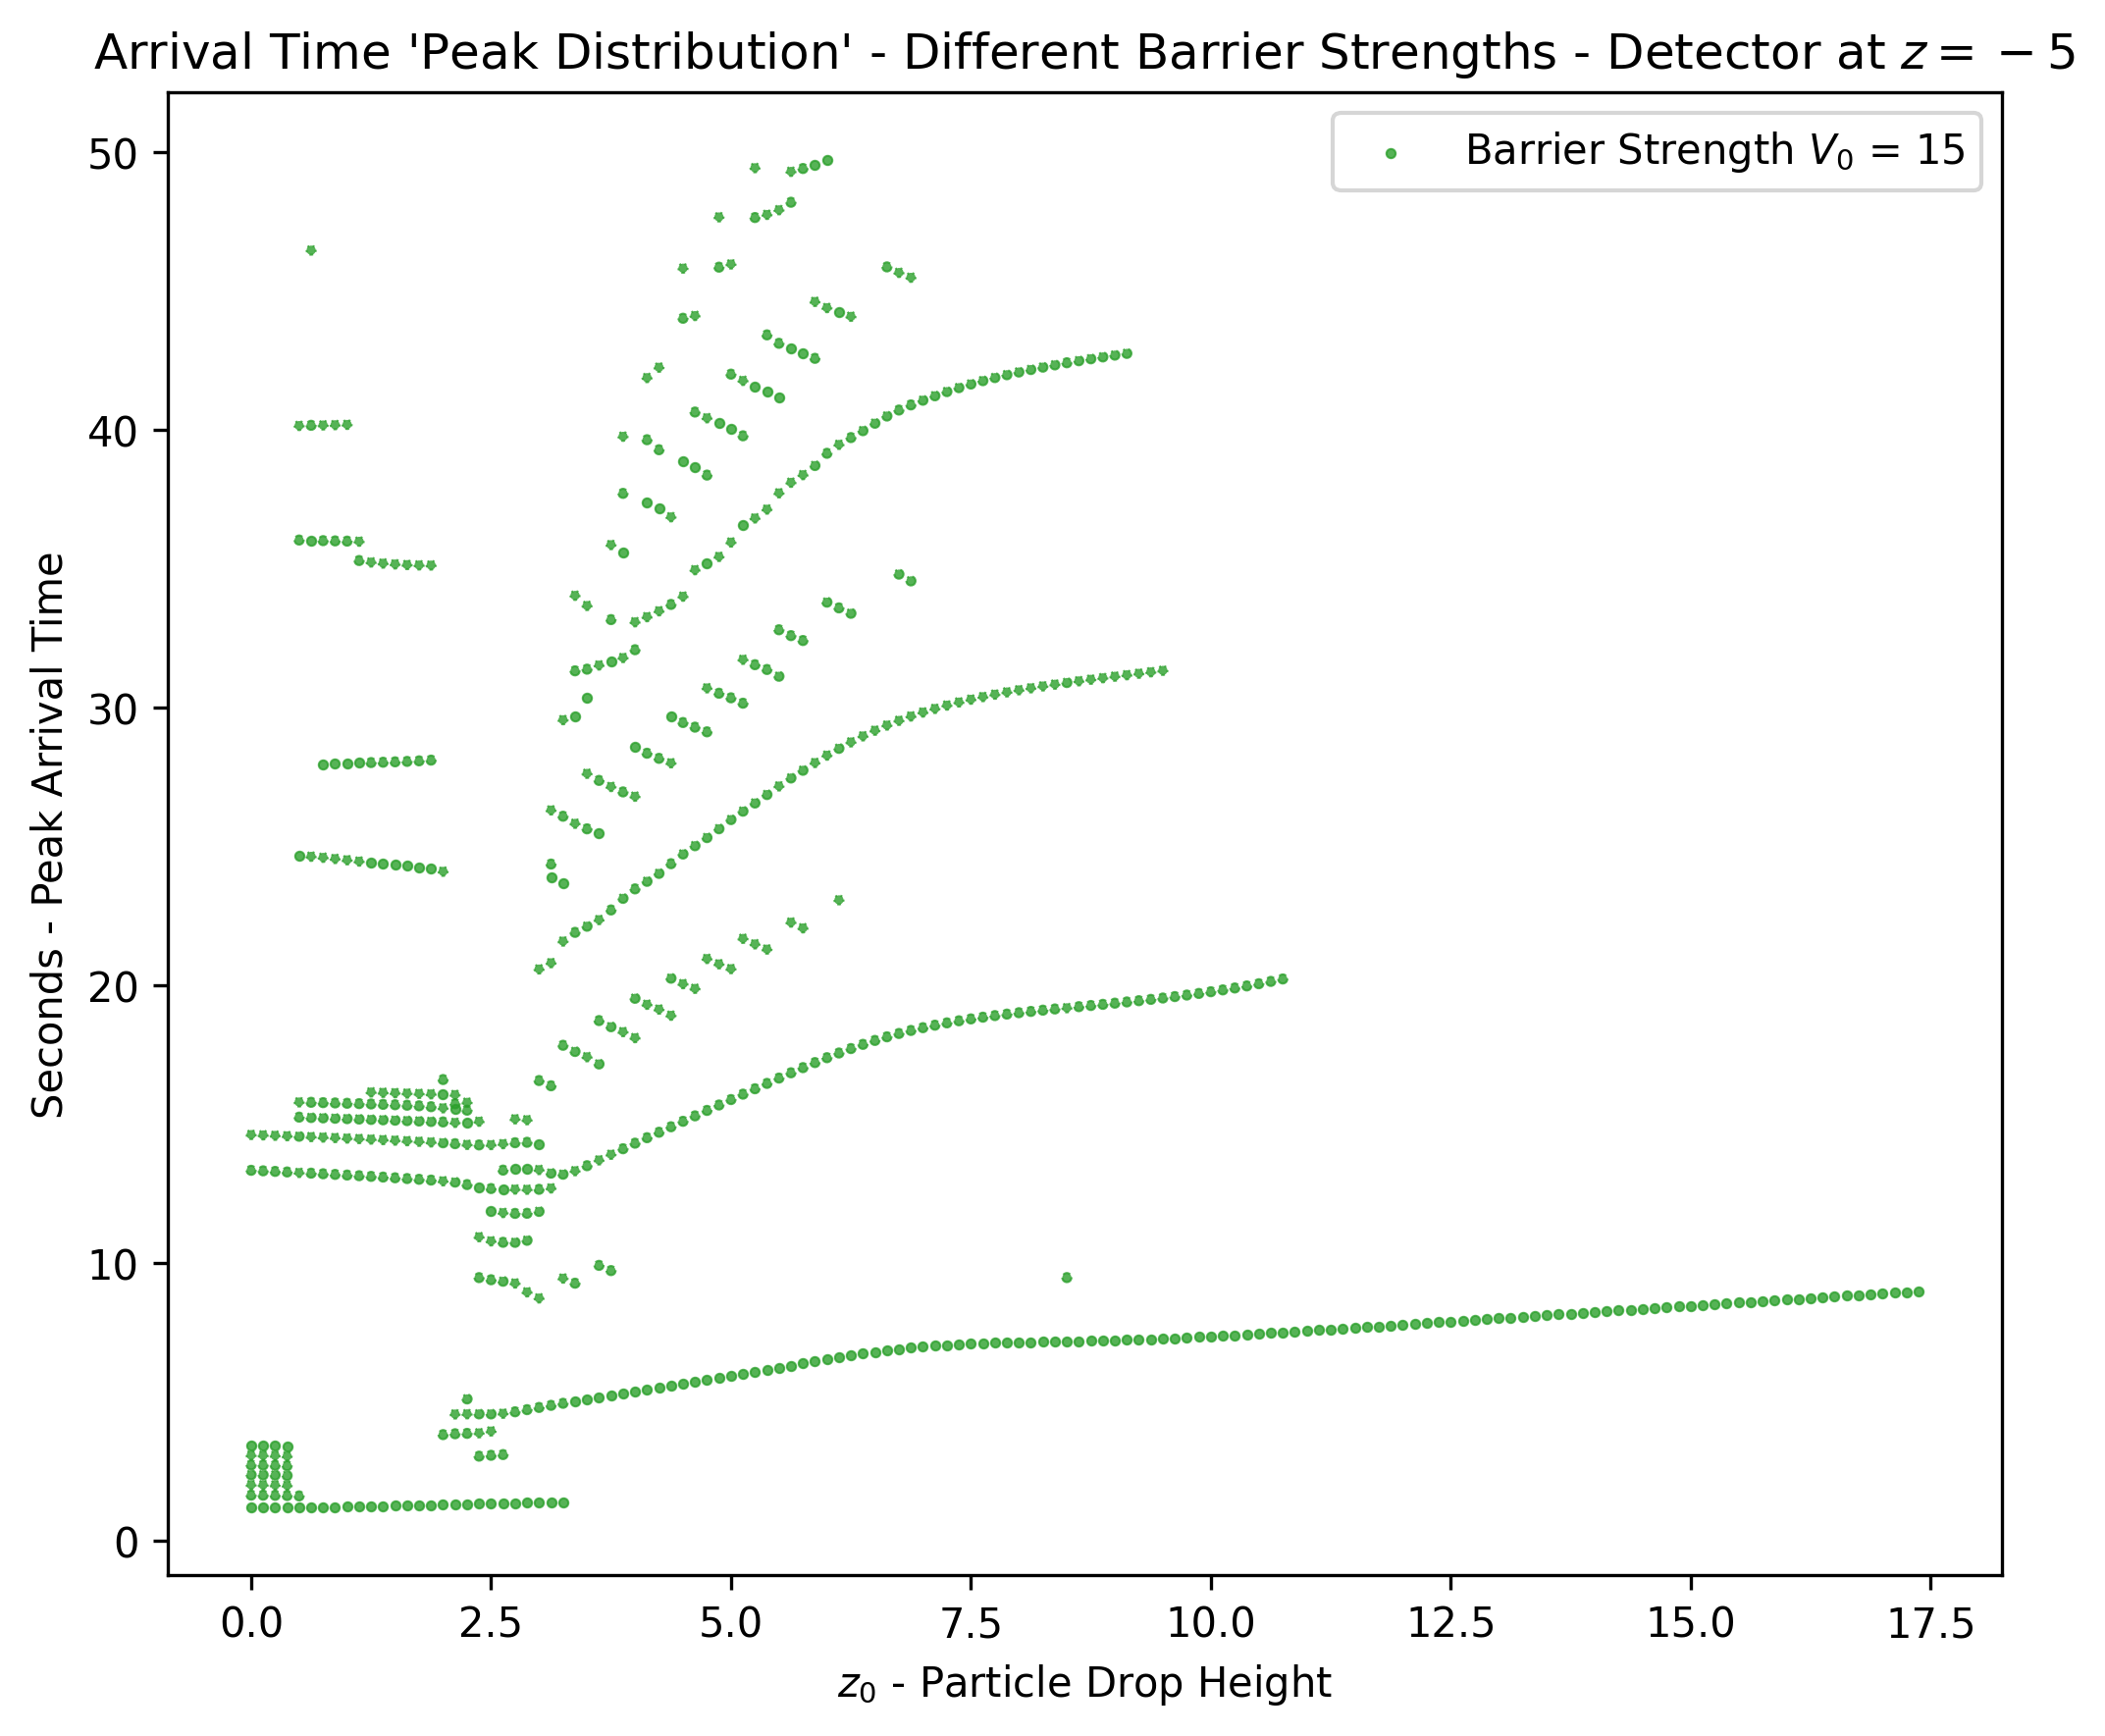
\includegraphics[width=1\linewidth]{Figures//Yoshida/6ea28a98-6d61-473d-b6d2-1cf271d0eed3.png}
    
    \caption{Peaks in Arrival Time \textbf{(seconds)} in Gaussian barriers for isolated cases, demonstrating the non-linear effects of the simple setup.}
    \label{fig:zr1r1r1}
\end{figure}

\begin{figure}
    \centering
    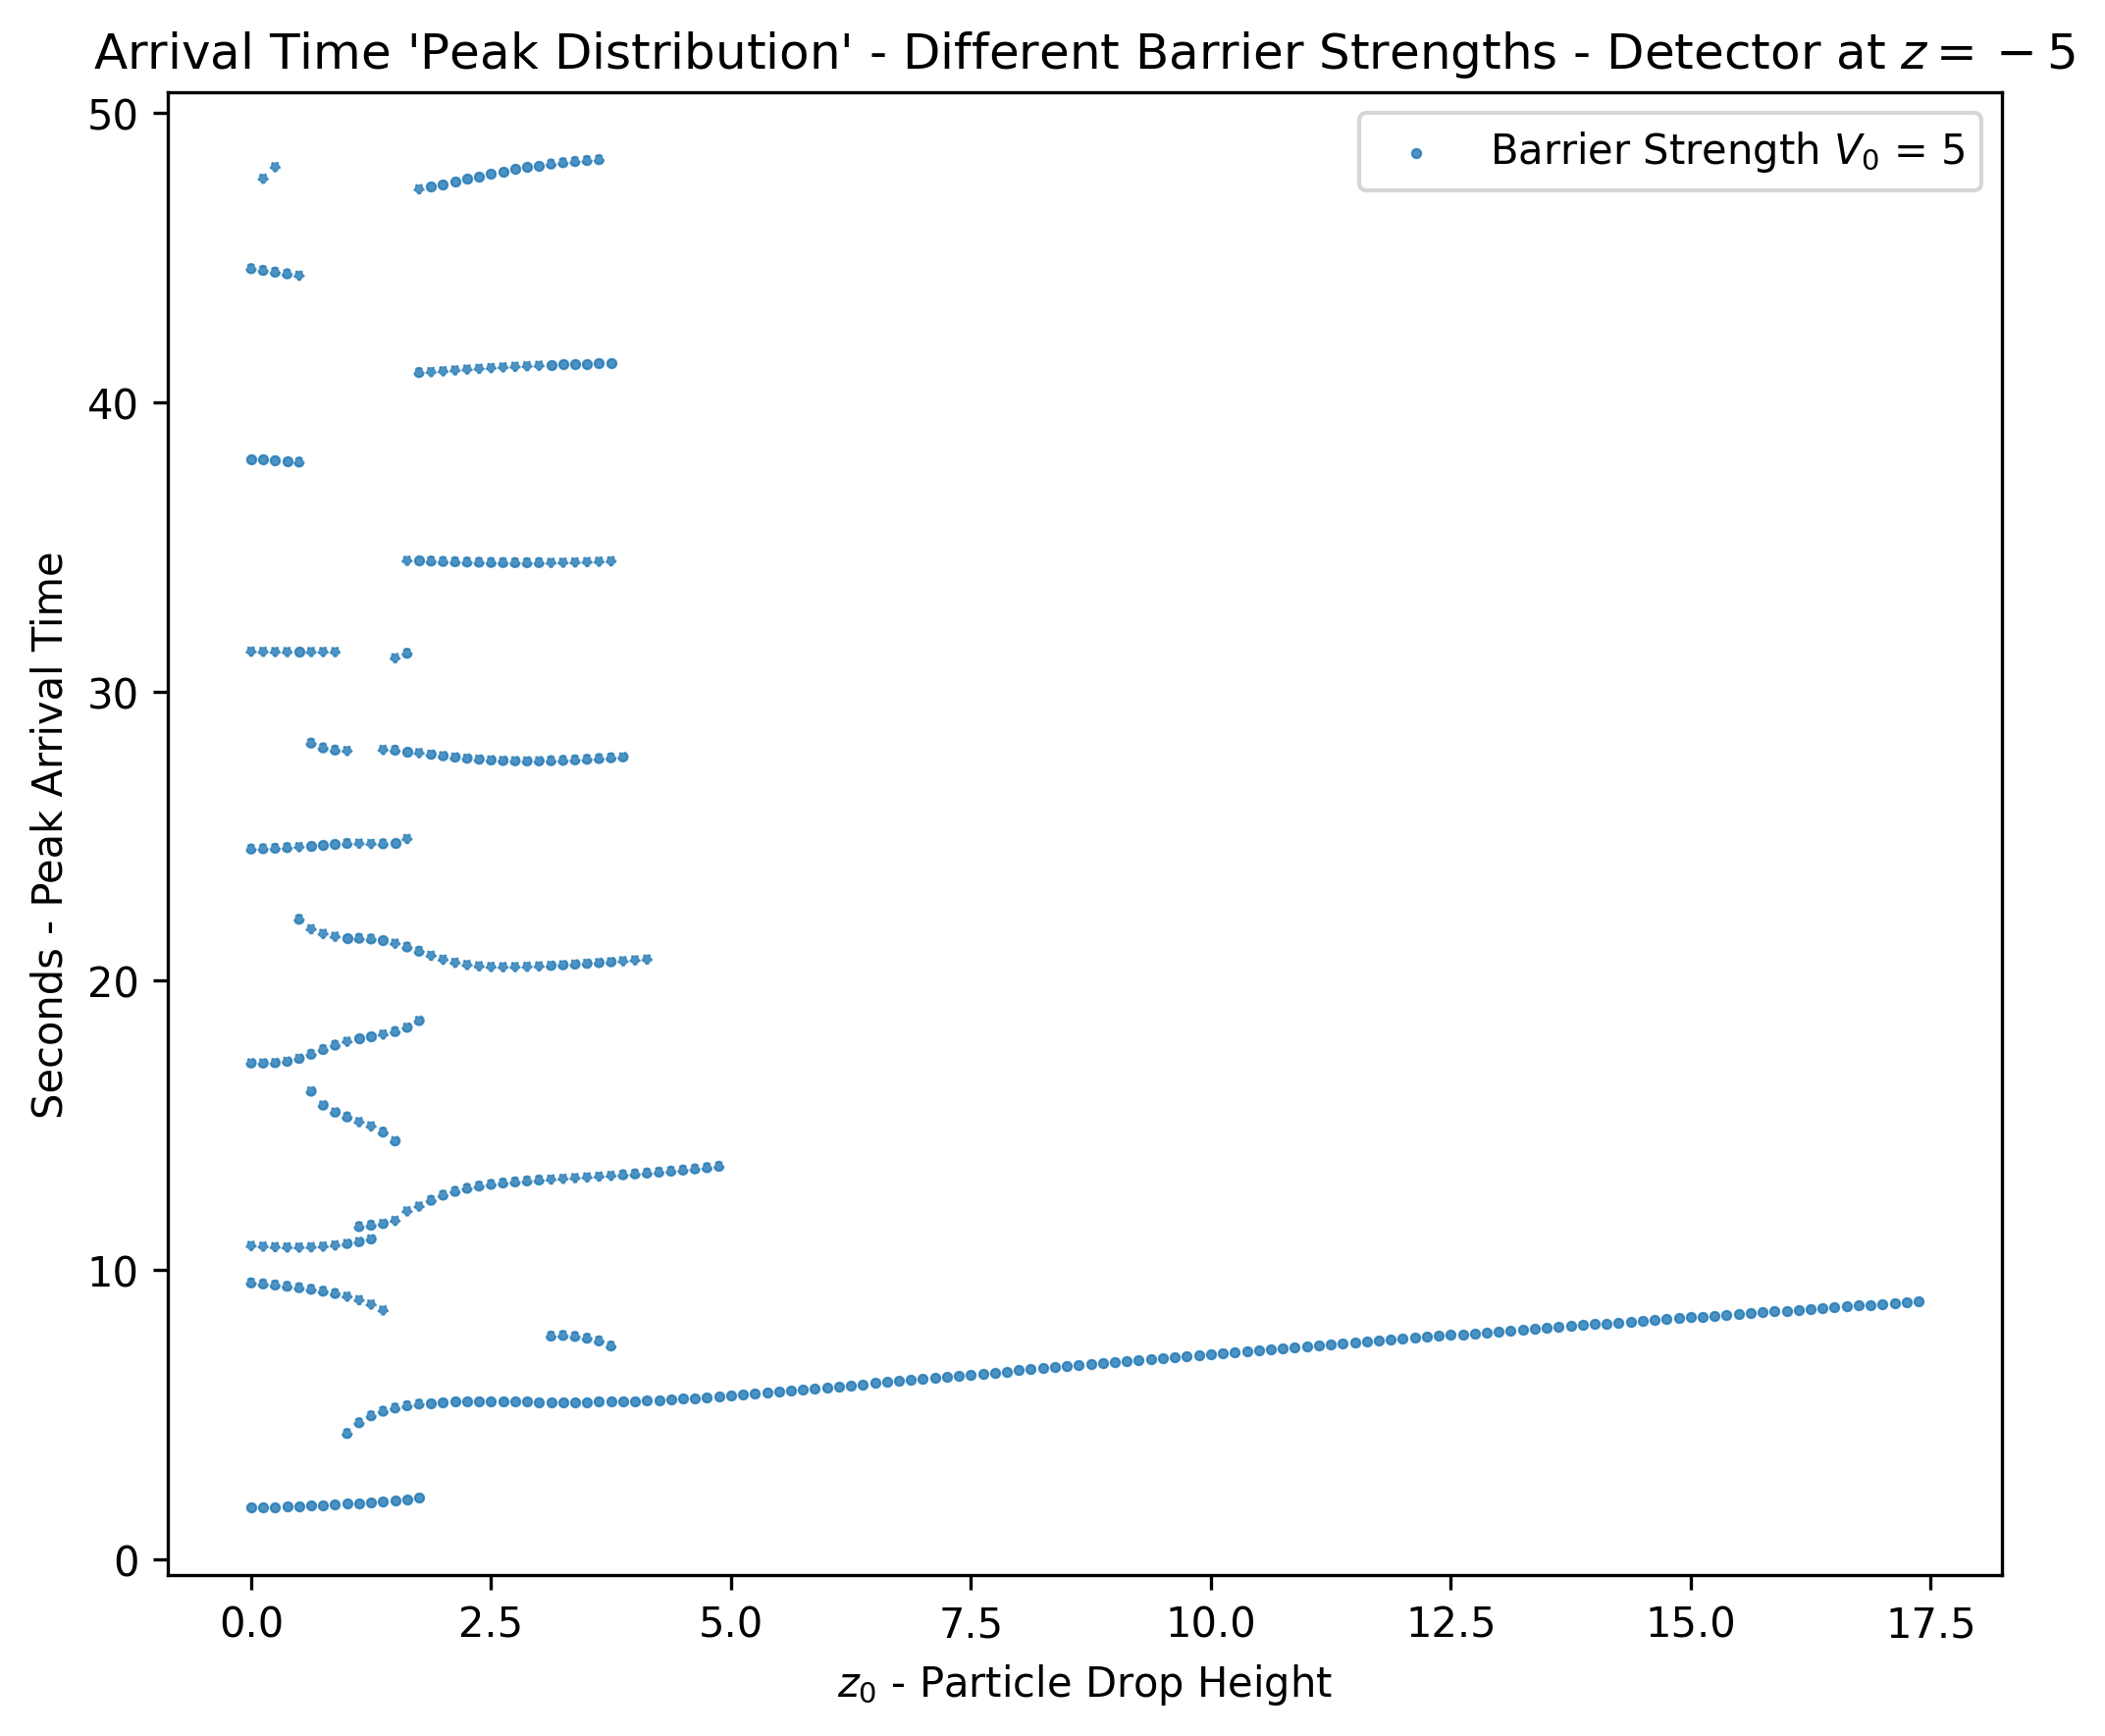
\includegraphics[width=1\linewidth]{Figures//Yoshida/a1bd2b6c-81f9-41d3-8438-e17ff23907c9.png}
    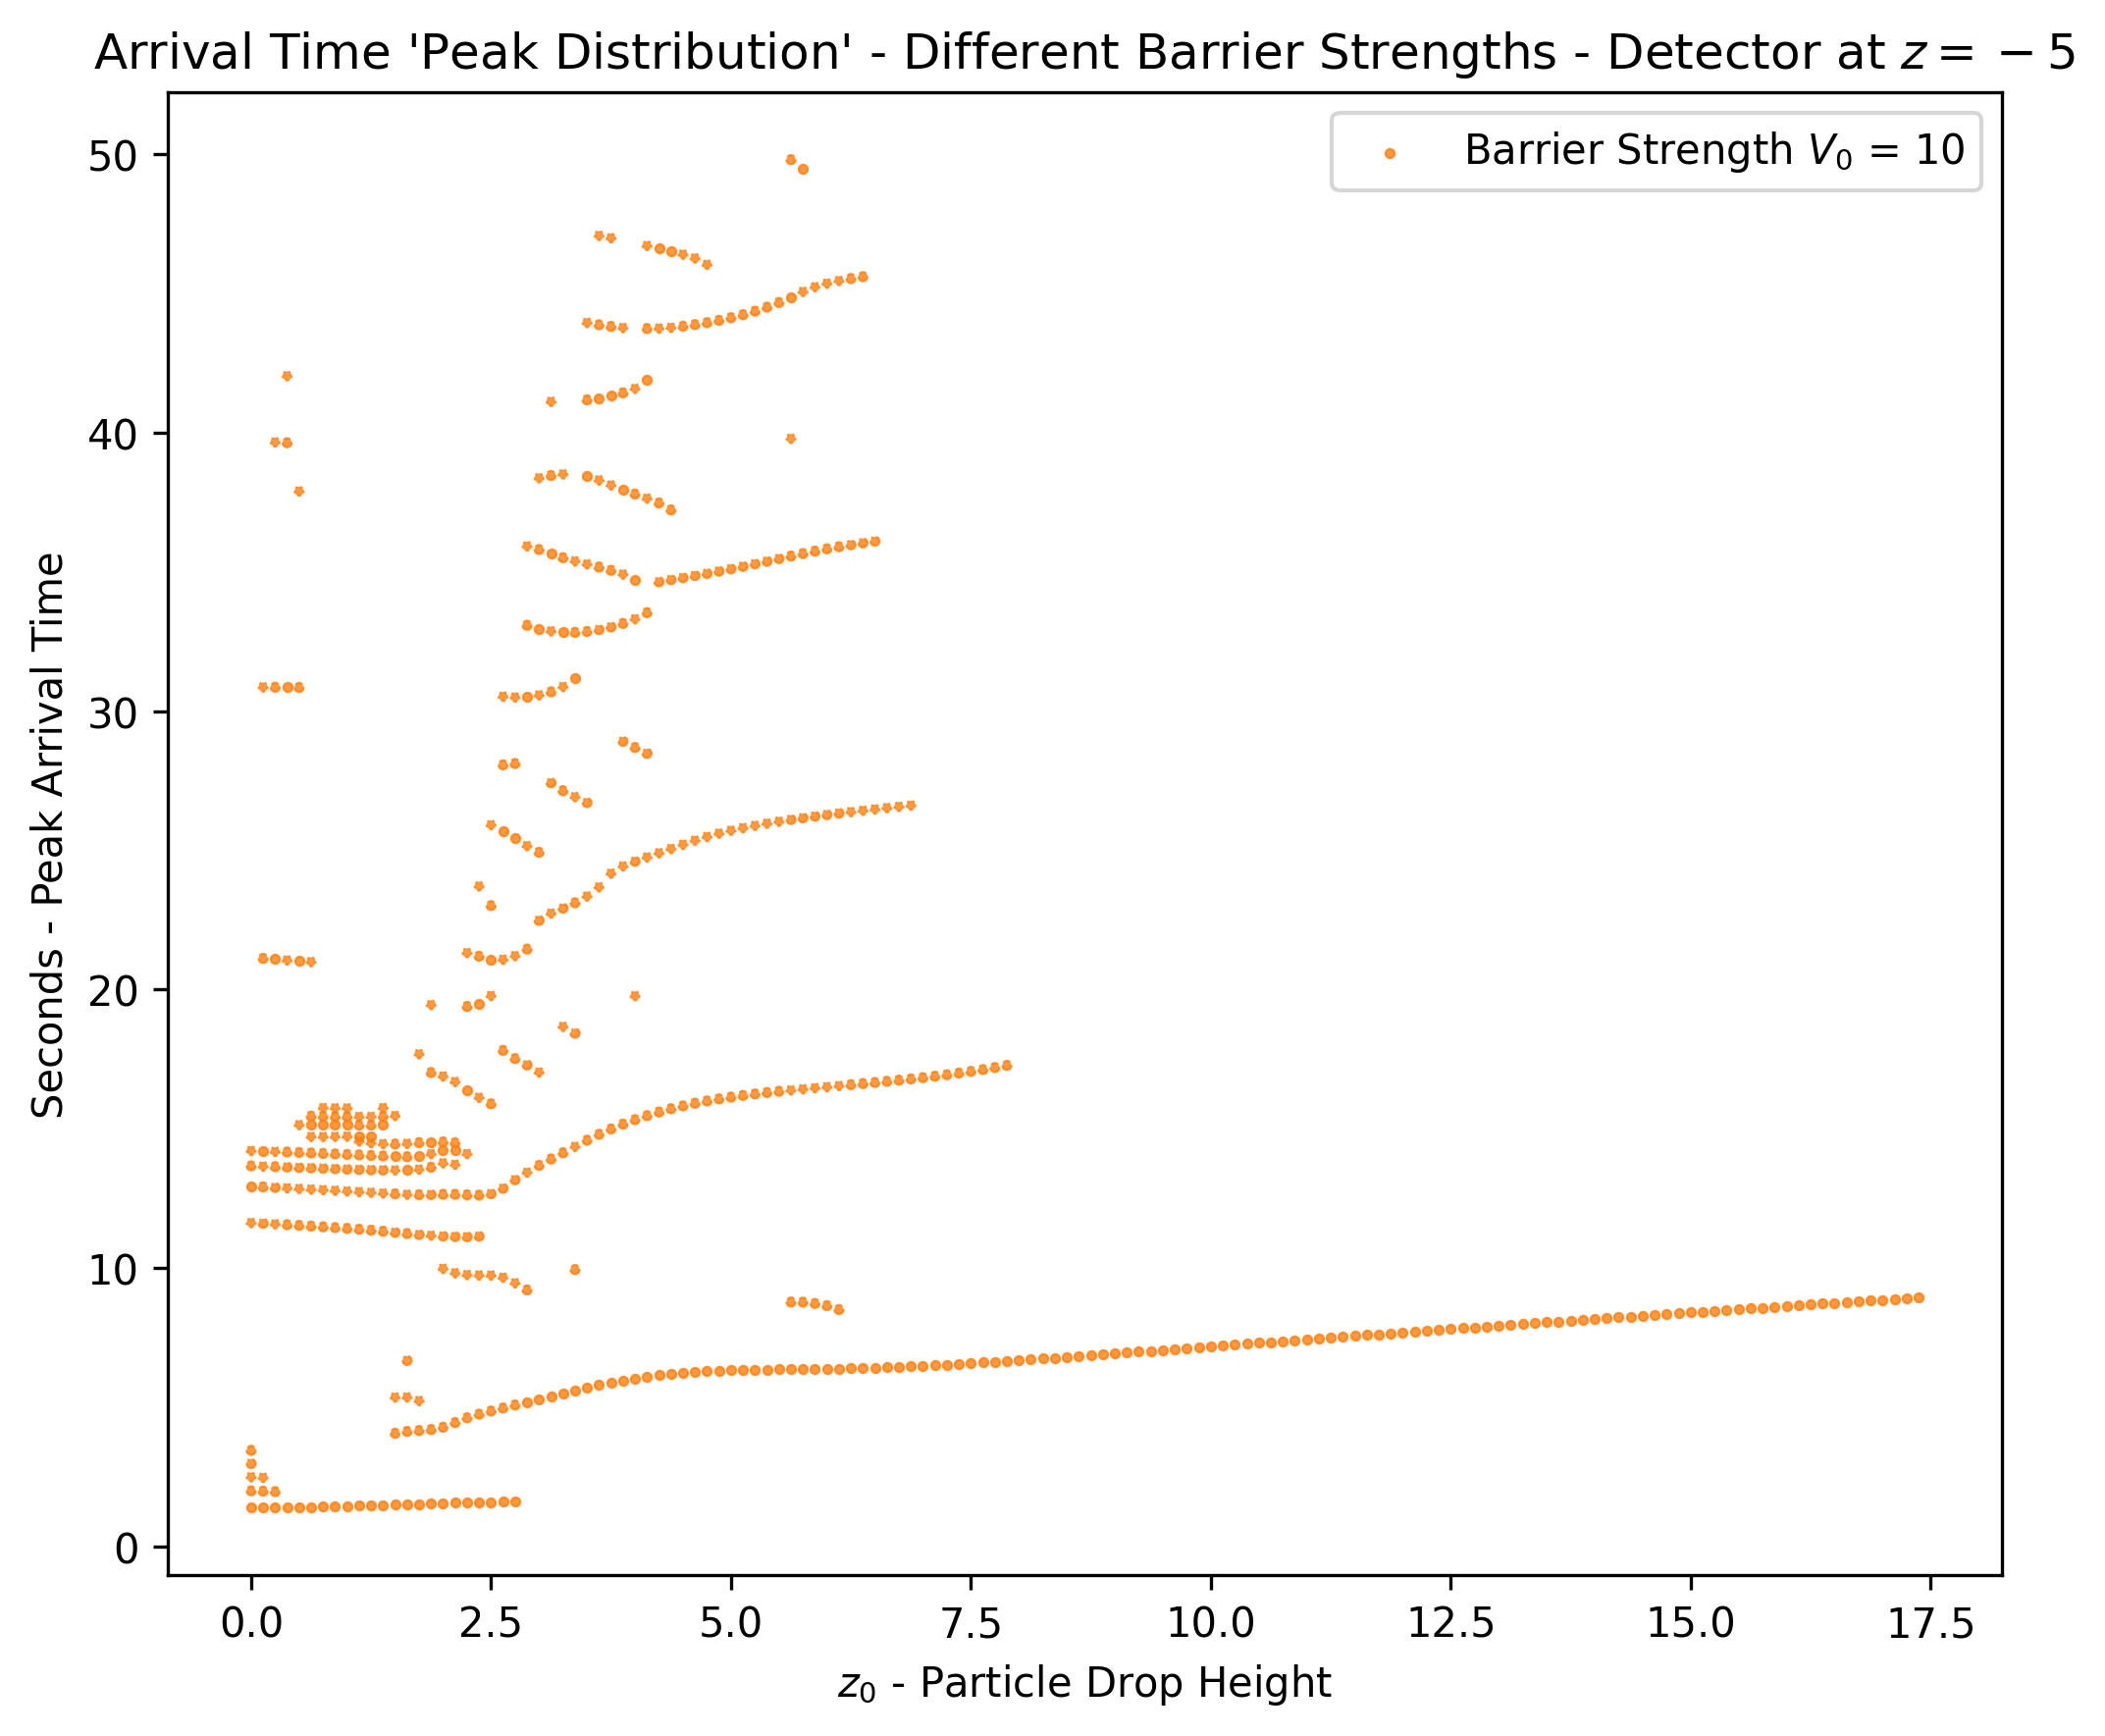
\includegraphics[width=1\linewidth]{Figures//Yoshida/8001f847-4d00-4d21-9122-b9a3feeb351c.png}
    
    \caption{Peaks in Arrival Time \textbf{(seconds)} in Gaussian barriers for isolated cases, demonstrating the non-linear effects of the simple setup.}
    \label{fig:f3f1fa}
\end{figure}

% Current intensity 
\begin{figure}
    \centering
    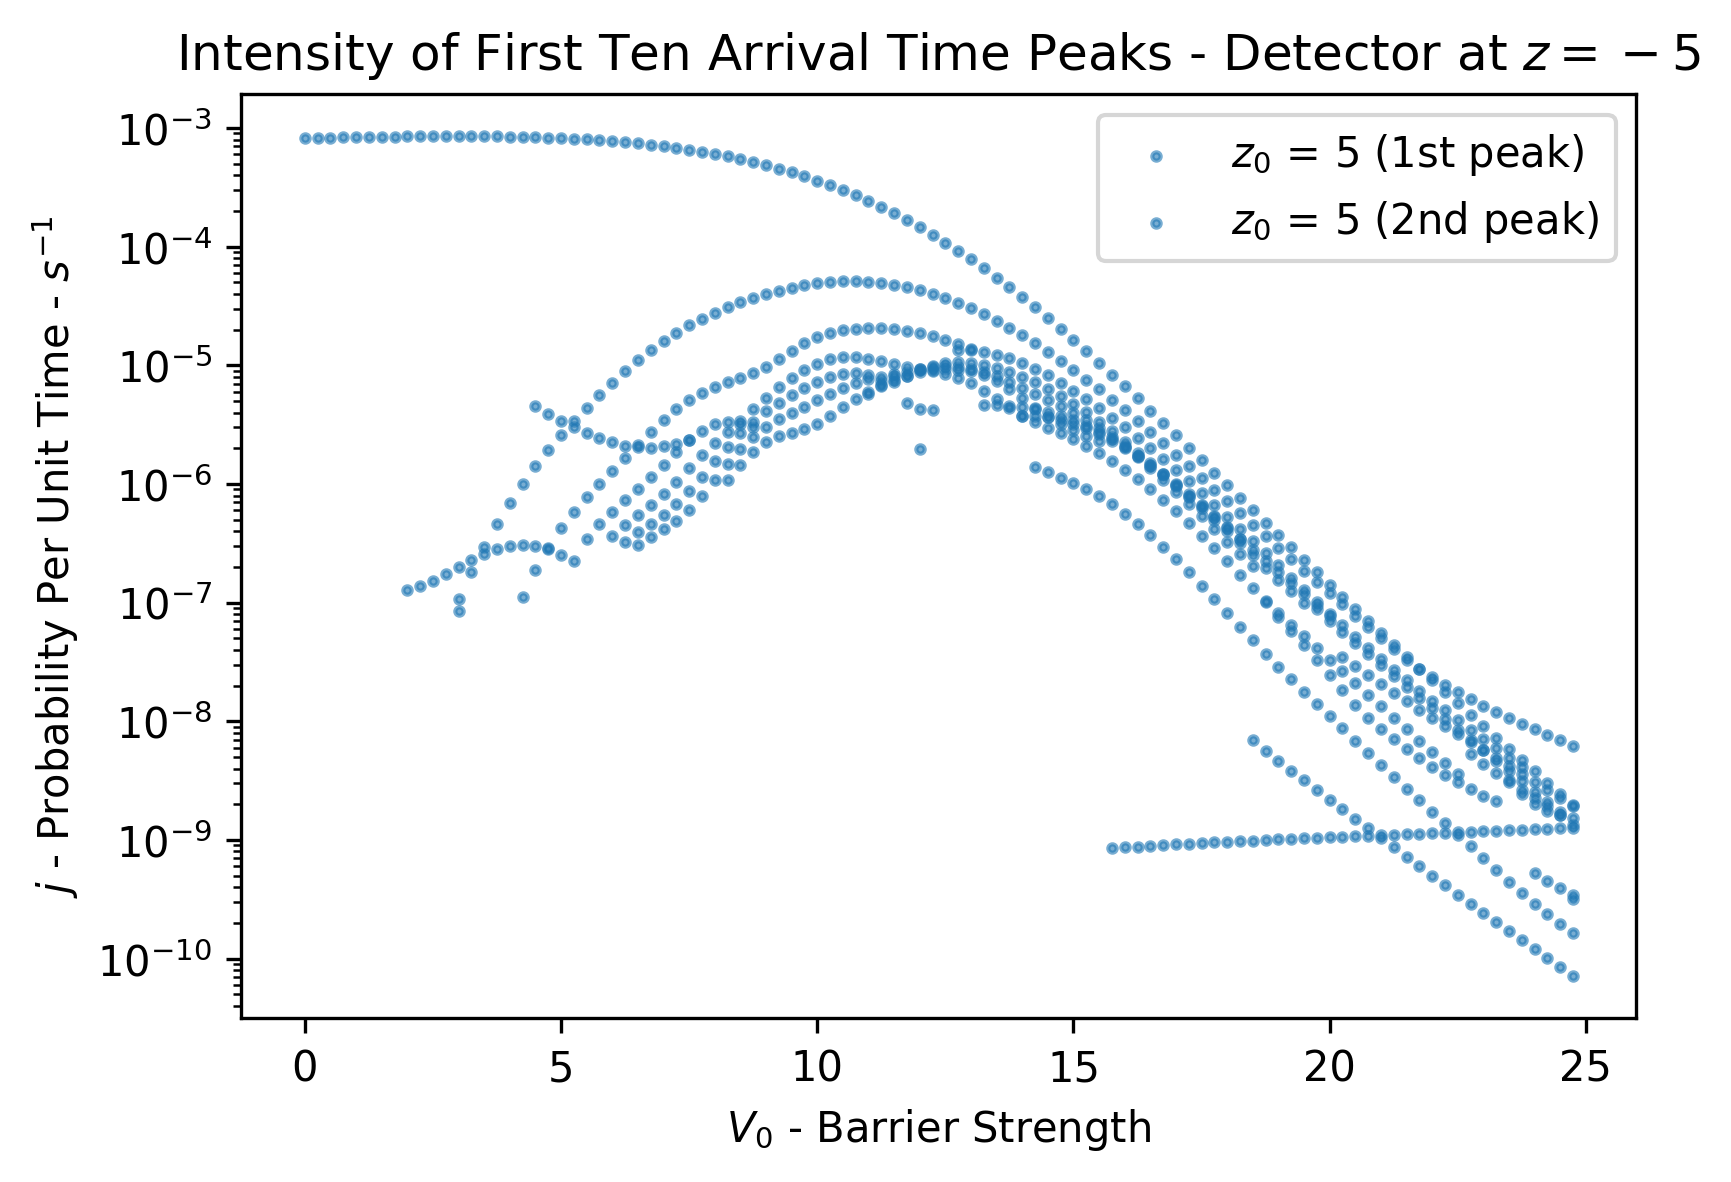
\includegraphics[width=1\linewidth]{Figures//Yoshida/315bac72-2cf4-490a-a645-c4bb62402058.png}
    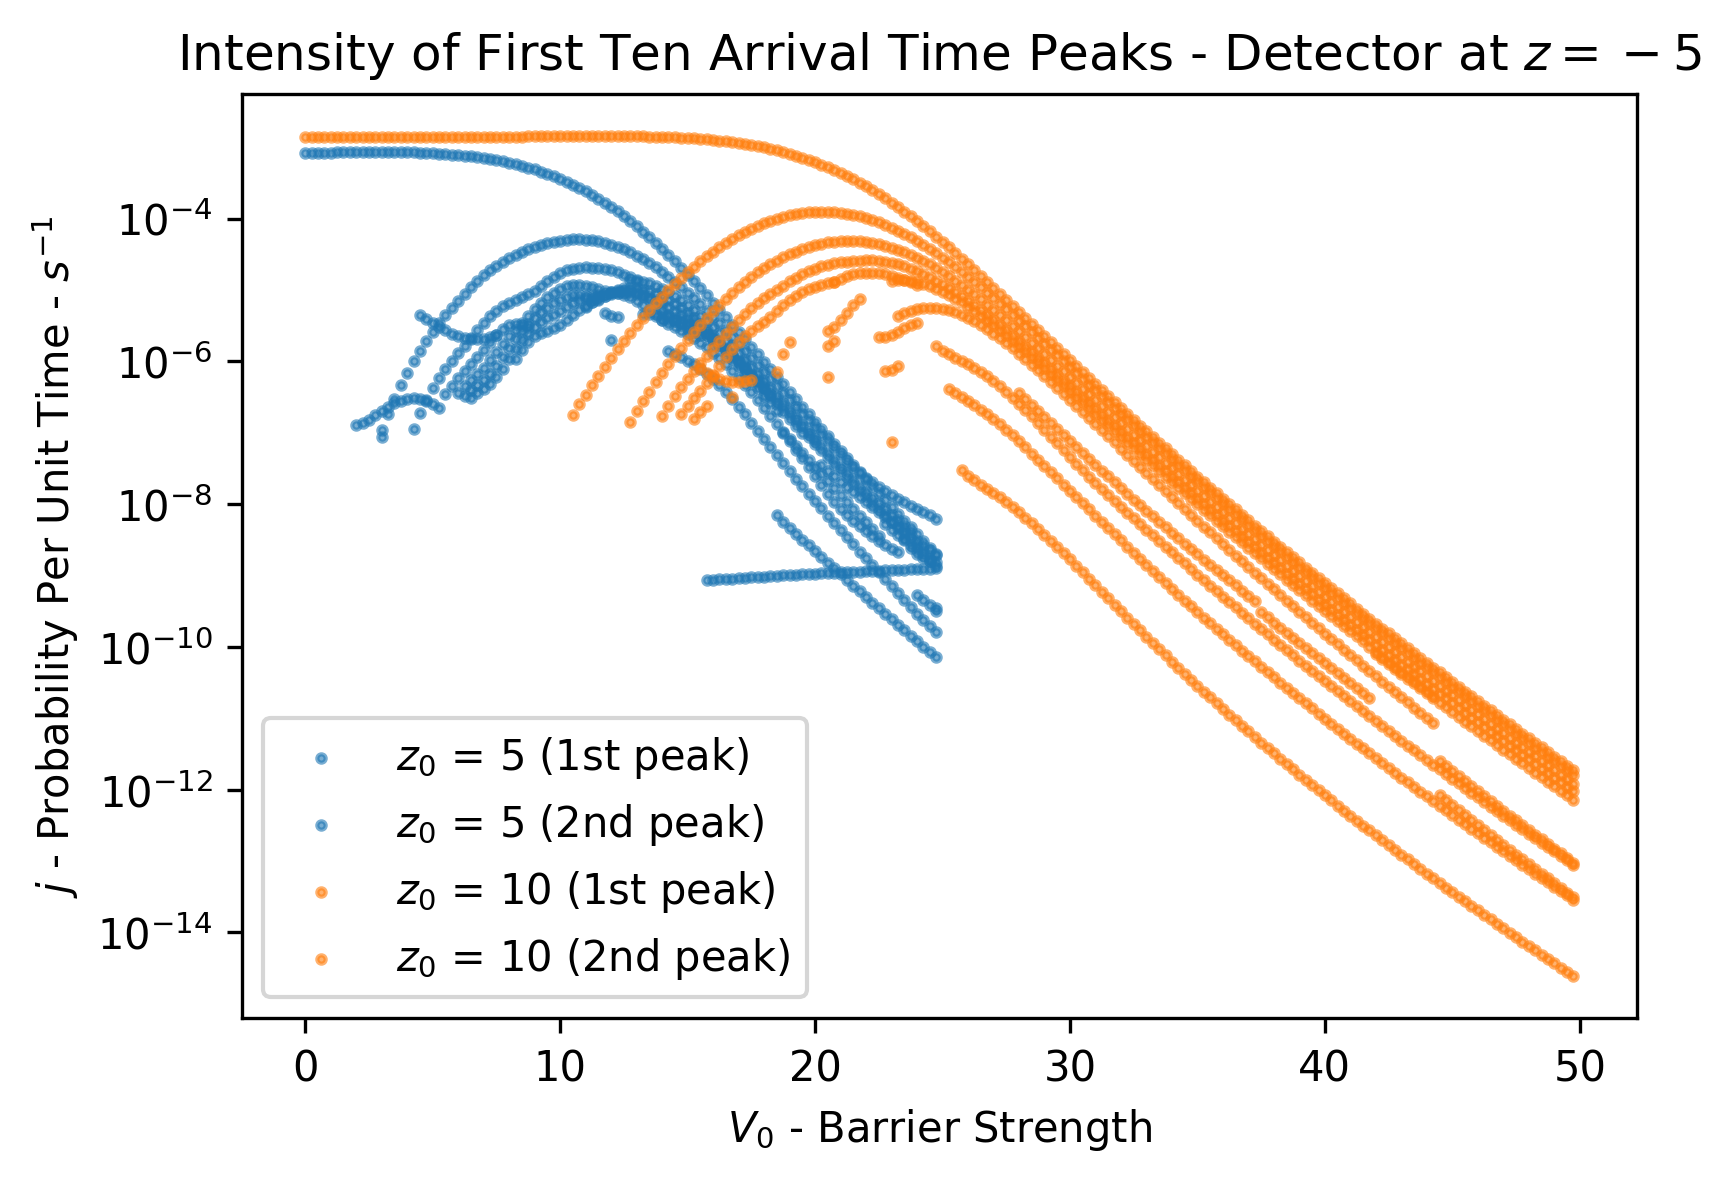
\includegraphics[width=1\linewidth]{Figures//Yoshida/3e1e8d24-1012-4fbe-ab70-c78f2fe41e39.png}
    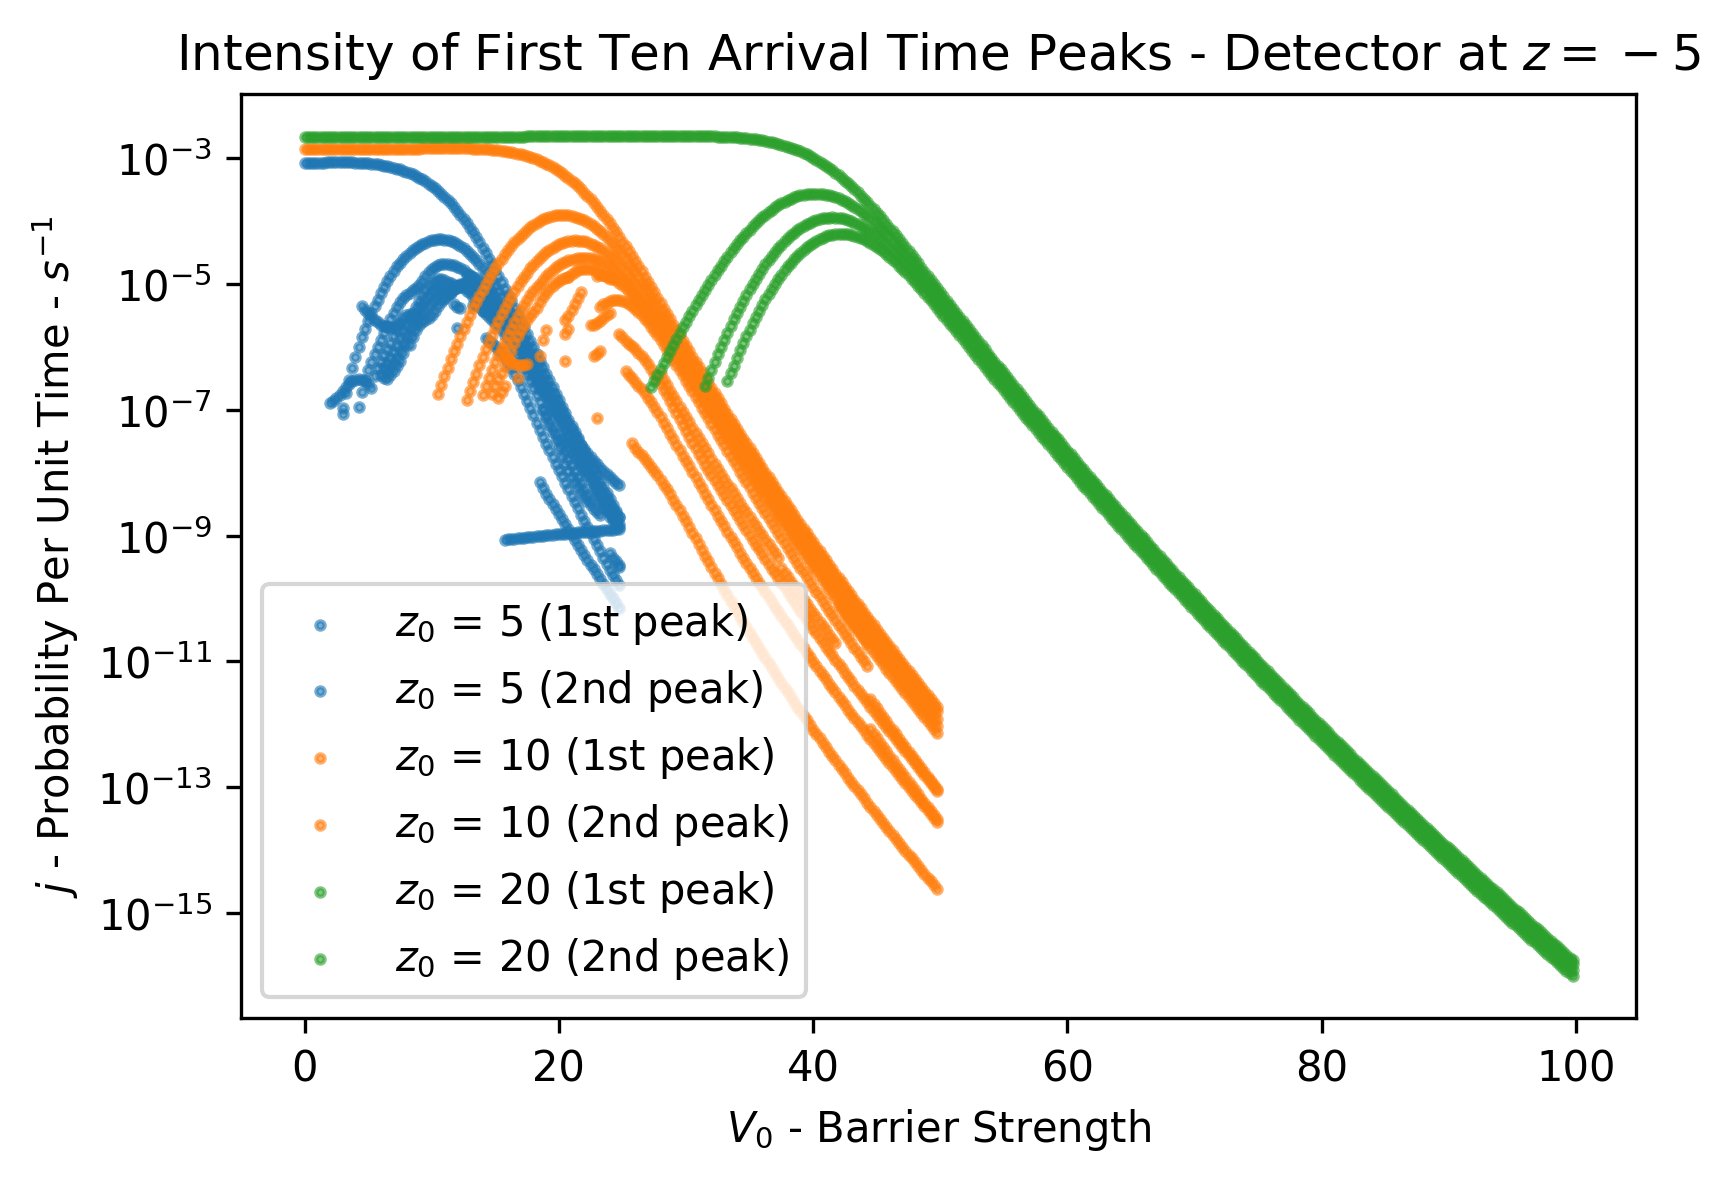
\includegraphics[width=1\linewidth]{Figures//Yoshida/2897f6b7-dd93-43e5-8846-e3fb0f150b28.png}
    
    \caption{Peaks in Arrival Time \textbf{(Intensity)} Distribution, already shown before, here displayed in individually highlighted cases. On the upper graph, notice this particular "weaving" of the fourth arrival (count from top) at coordinate (12; $7\times10^{-6}$) for the blue region. A clear resonant point is forming there, as in all other barrier strengths, multiple arrival time peaks have been witnessed.}
    \label{fig:abc123}
\end{figure}

\begin{figure}
    \centering
    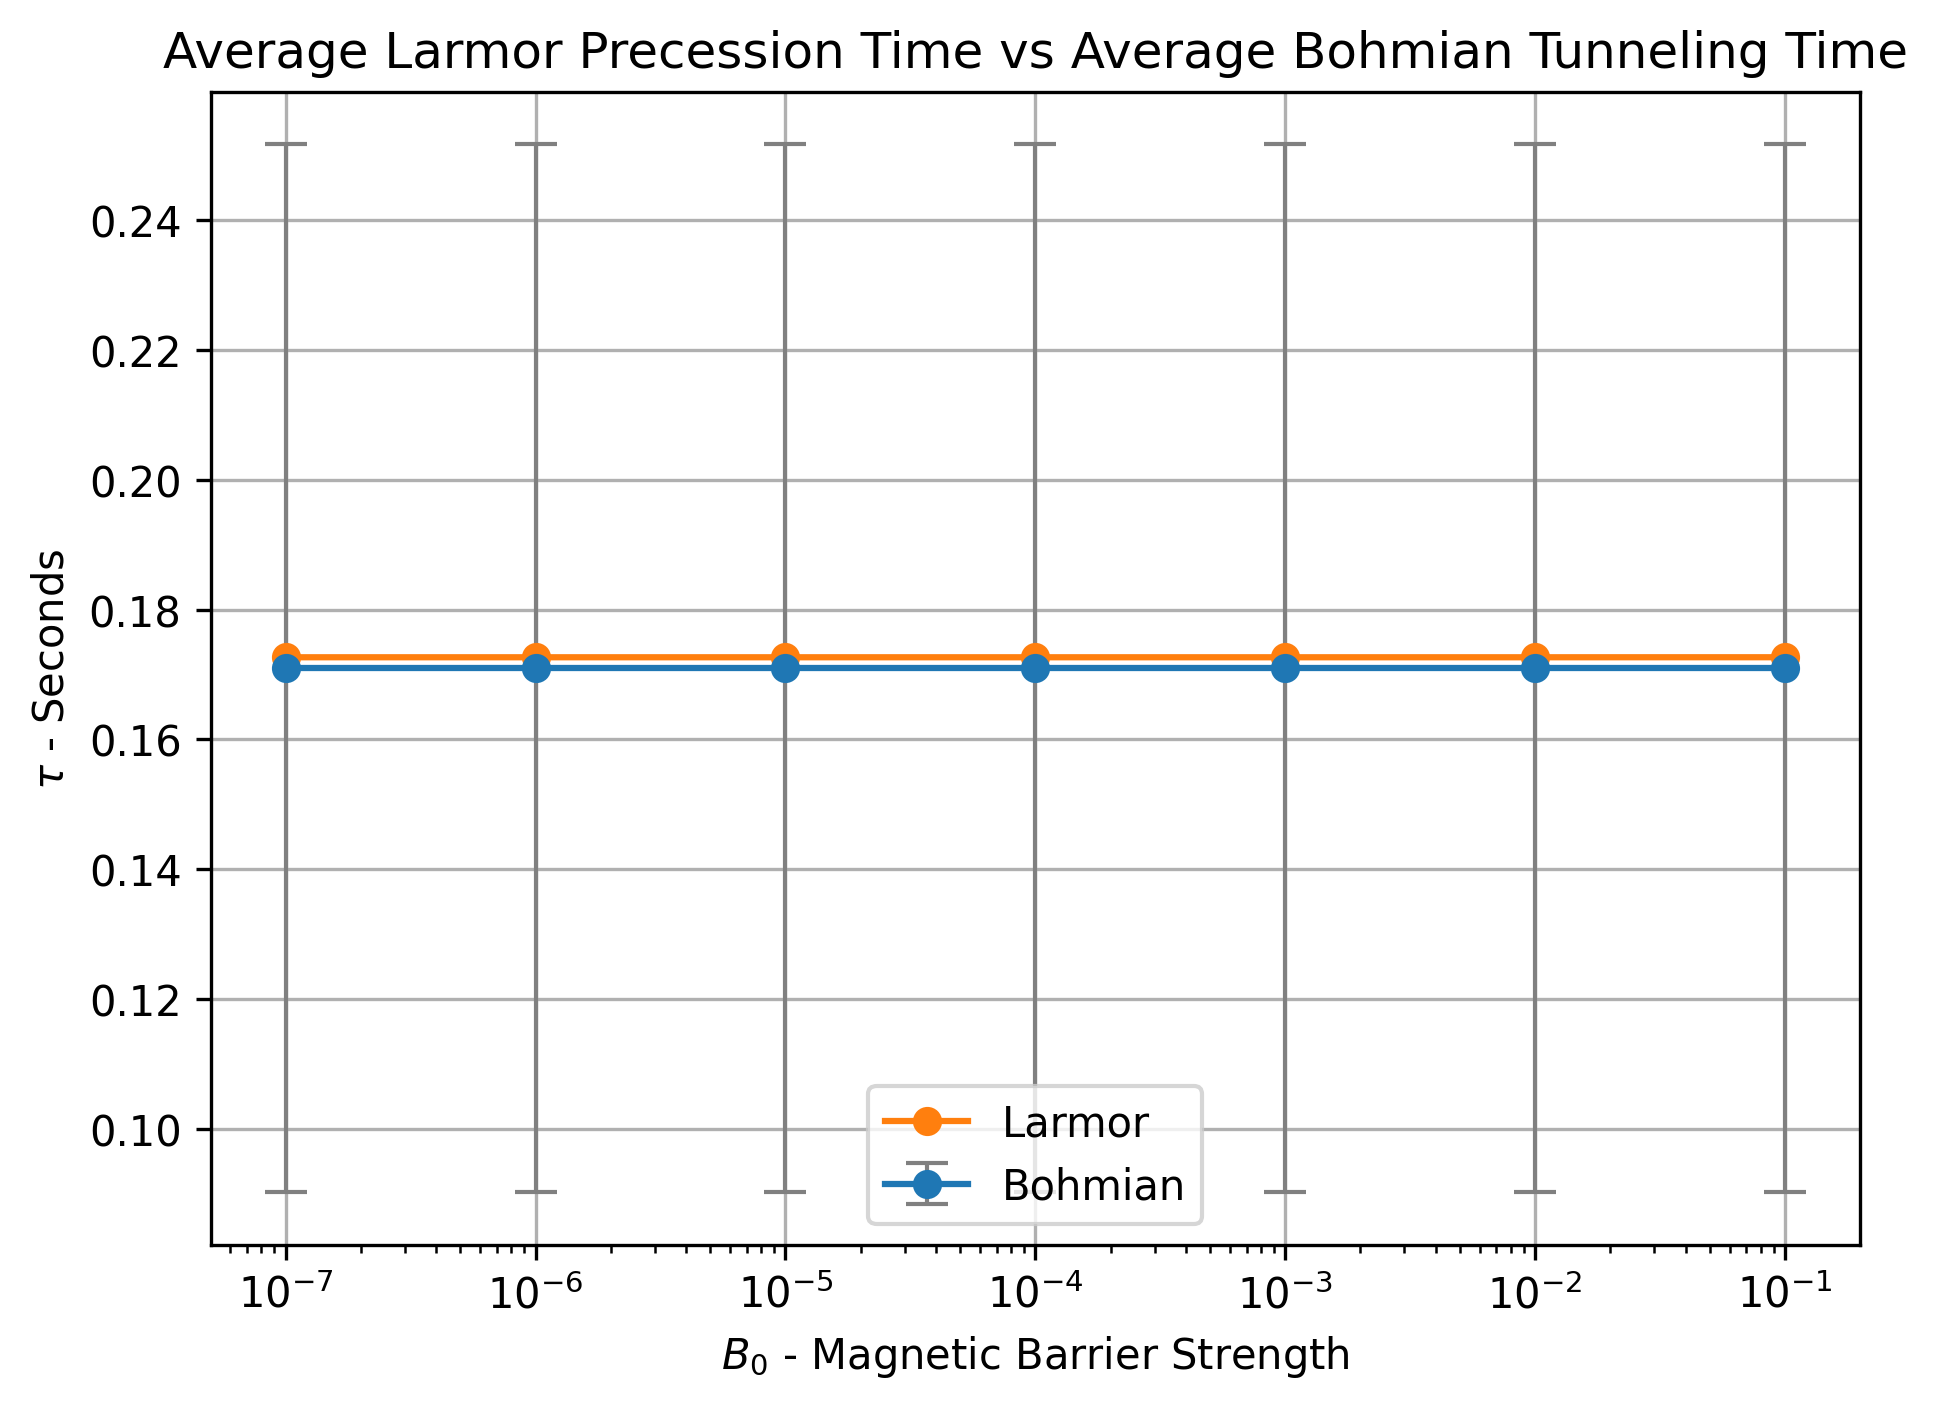
\includegraphics[width=1\linewidth]{Figures//2dspin/353e2f92-95a8-4c1b-b7b5-79fe511d7af9.png}
    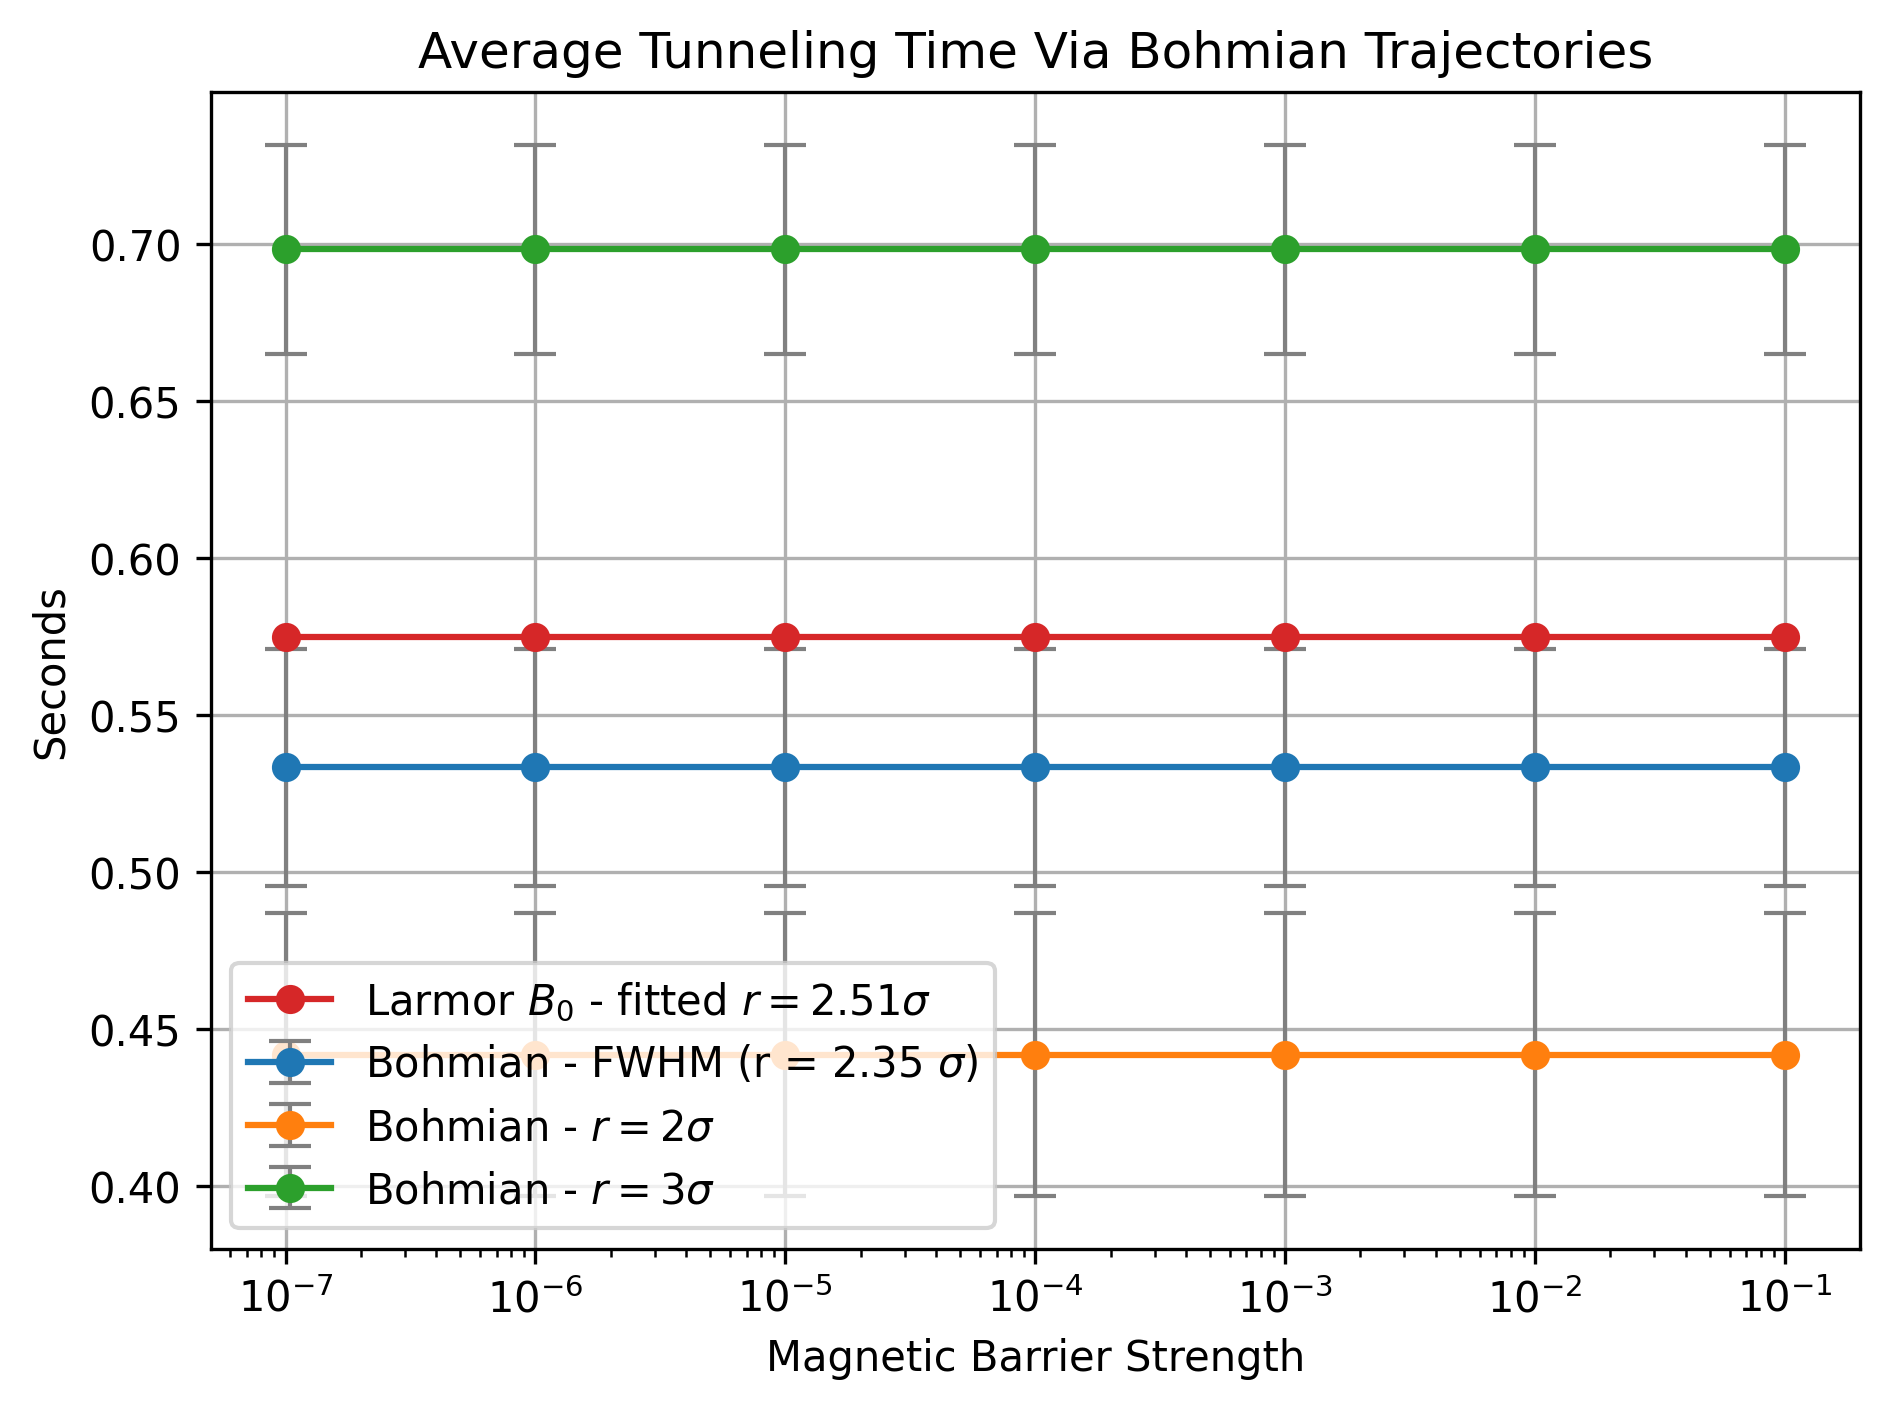
\includegraphics[width=1\linewidth]{Figures//2dspin/70557699-091f-4e39-a011-df61dbb7382d.png}
    
    \caption{Tunnelling Times For a Circular Uniform Barrier with a clear boundary (a), and a guassian barrier (b) both using Larmor Precession Times $\tau_L$, and bohmian trajectories. These data points are obtained in the weak field regime. At low magnetic strengths, the two seem to coincide. Error bars on the Bohmian tunnelling time represent 1 standard deviation.}
    \label{fig:tunneling_times}
\end{figure}

% Larmor vs Bohmian High Energy Regime
\begin{figure}
    \centering
    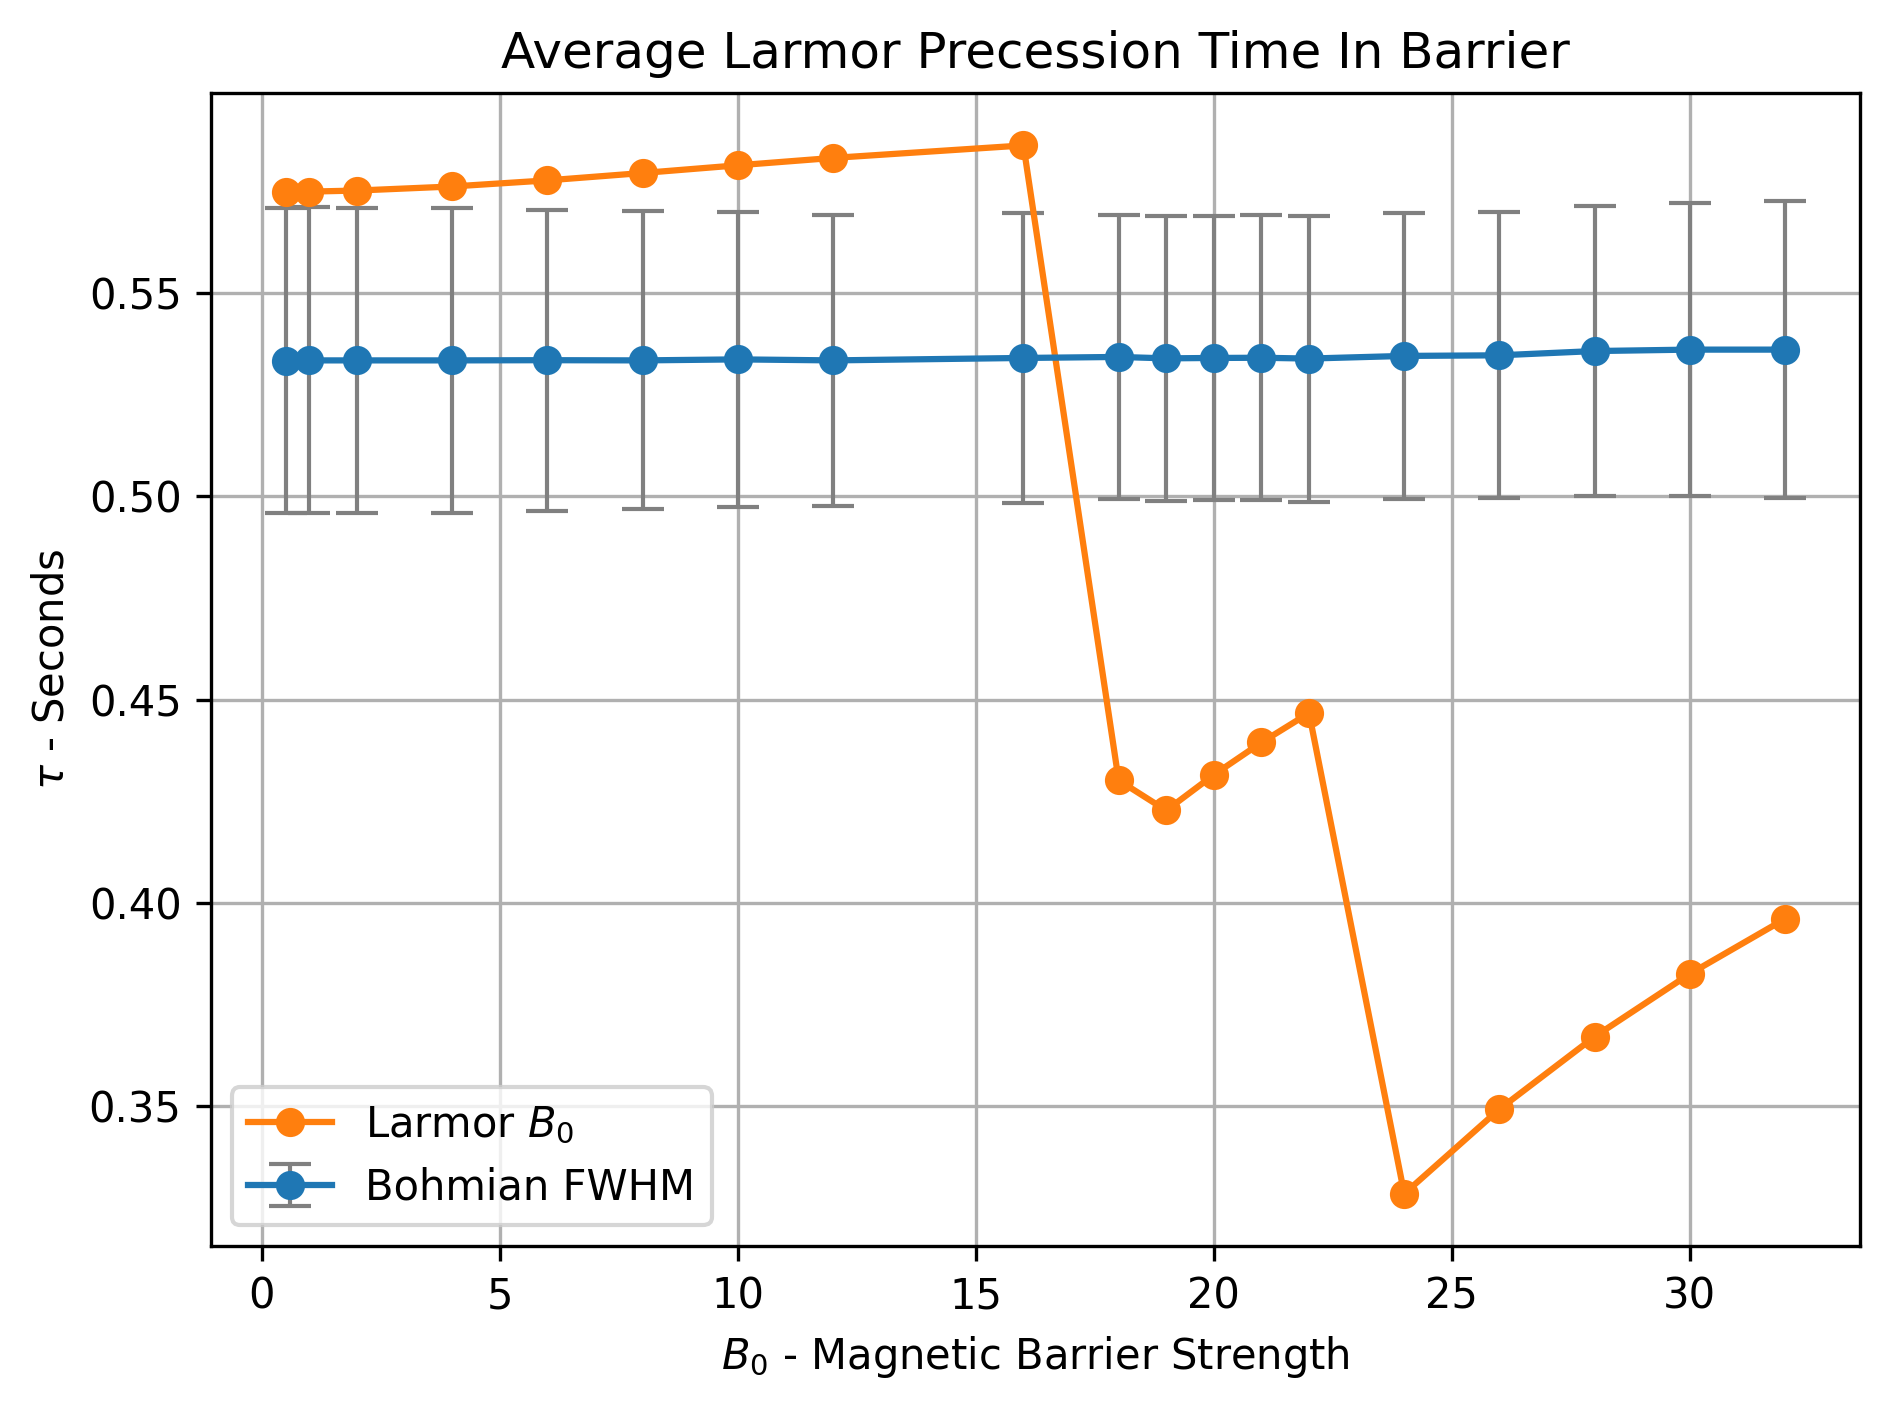
\includegraphics[width=1\linewidth]{Figures//2dspin/91acaee2-b8f1-495b-aa78-977150ff4034.png}
    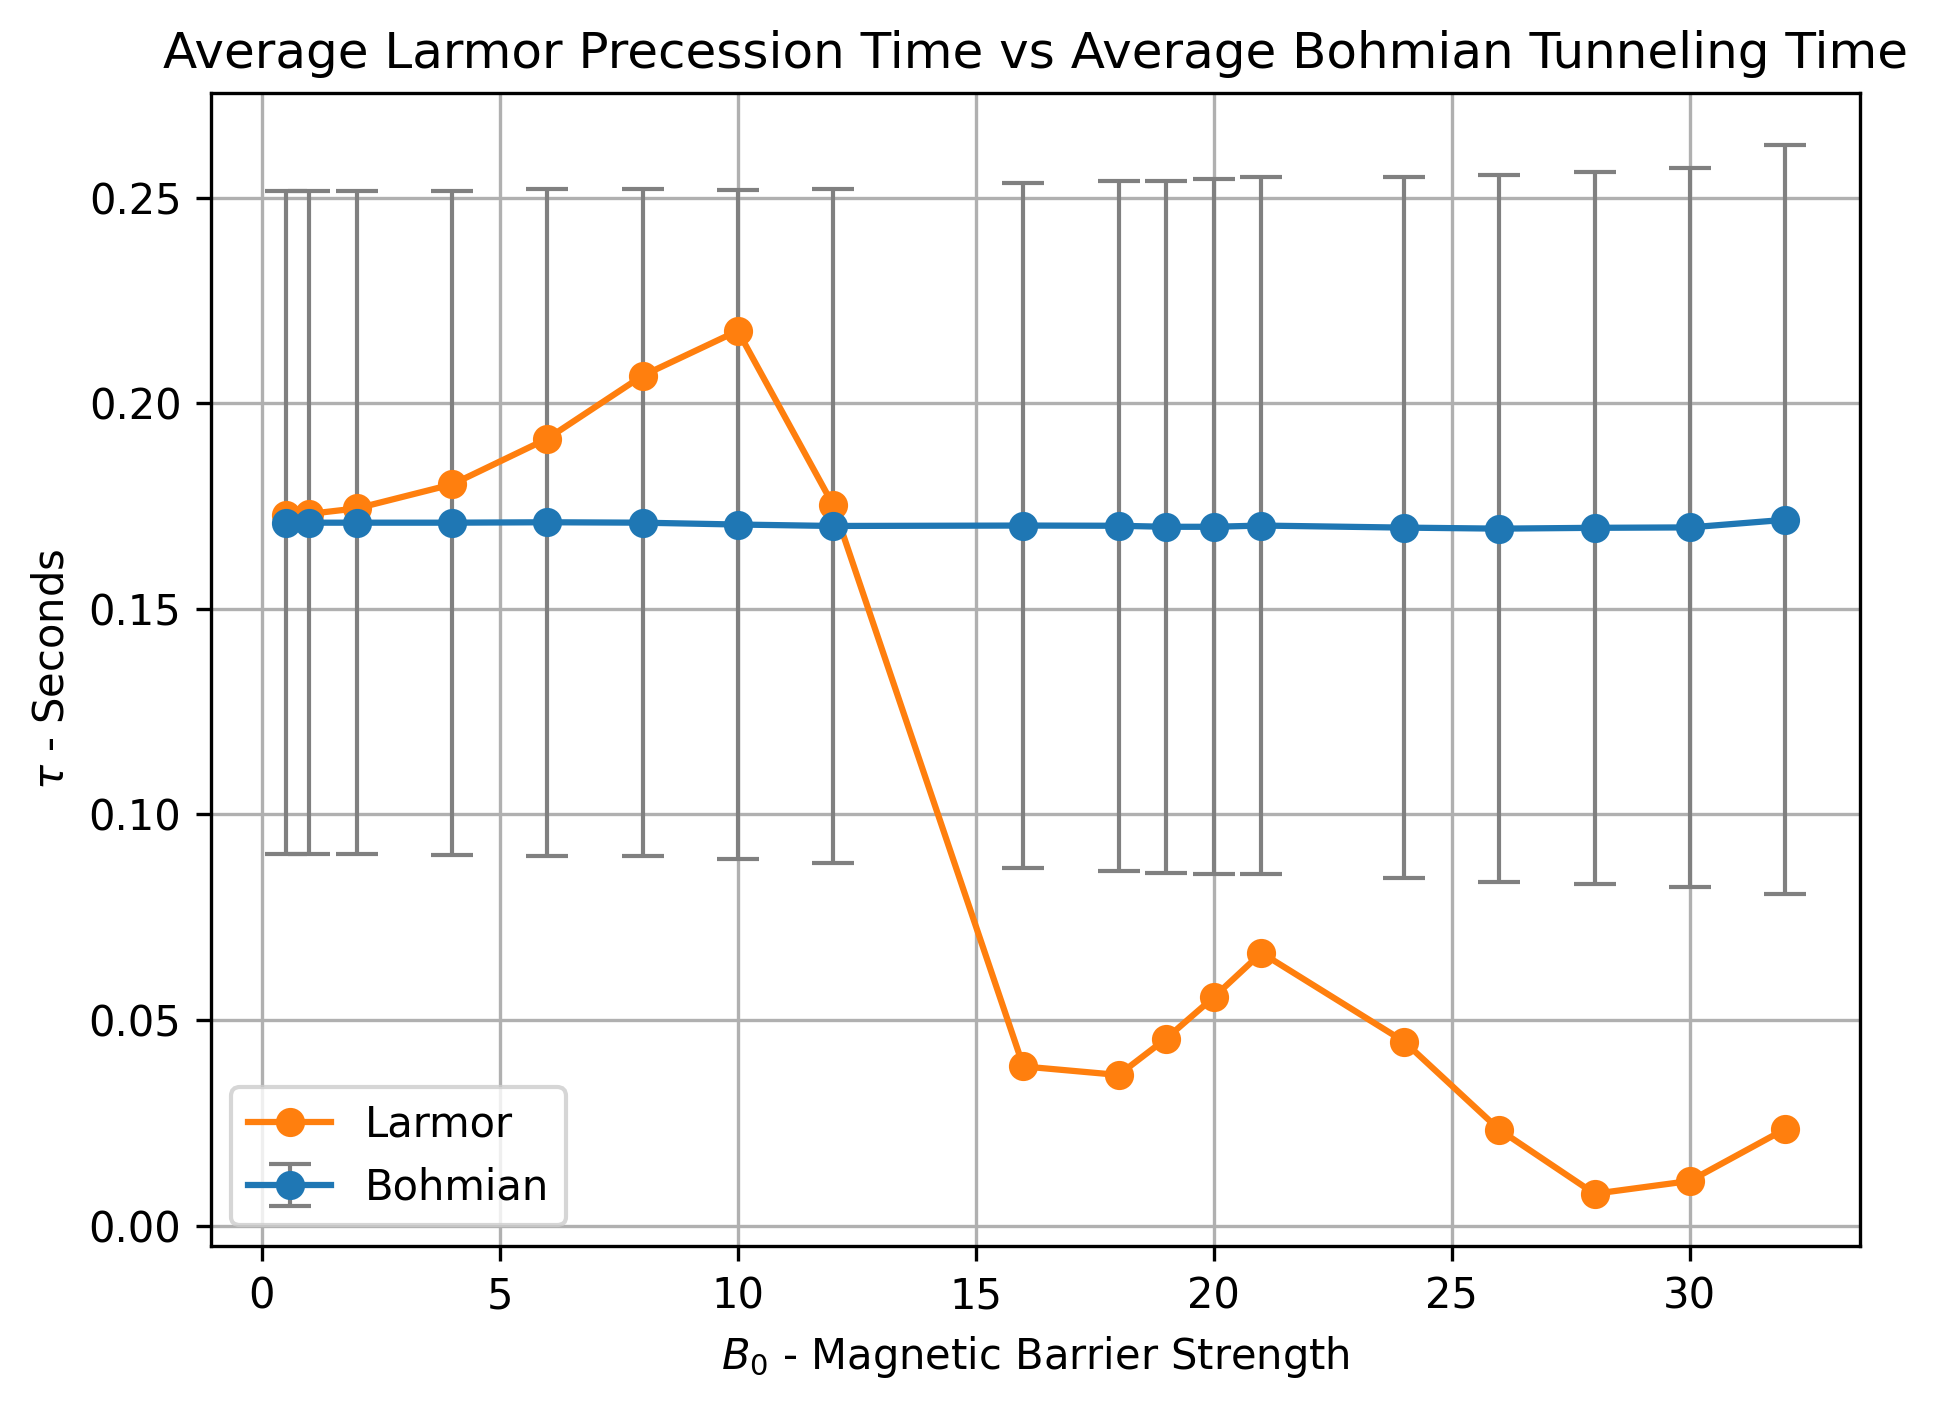
\includegraphics[width=1\linewidth]{Figures//2dspin/f62cf77c-707a-4972-834e-00b27fbb55db.png}
    
    \caption{Larmor Clock vs Bohmian Trajectories in strong magnetic field regime. Upper graph shows \textbf{gaussian barrier} tunneling times, with $2R=\text{2 ln (2) } \sigma$ (FHWM). Interestingly, the Bohmian tunneling time seem stable throughout, whereas the Larmor Clock quickly goes out of tilt. The lower figure shows the tunneling times for a circular (square-like) barrier. Here the tunneling times coincide in the low barrier strength regime (which is discussed in the main text of this study)}
    \label{fig:abc67rtyfugiop}
\end{figure}

\begin{figure}
    \centering
    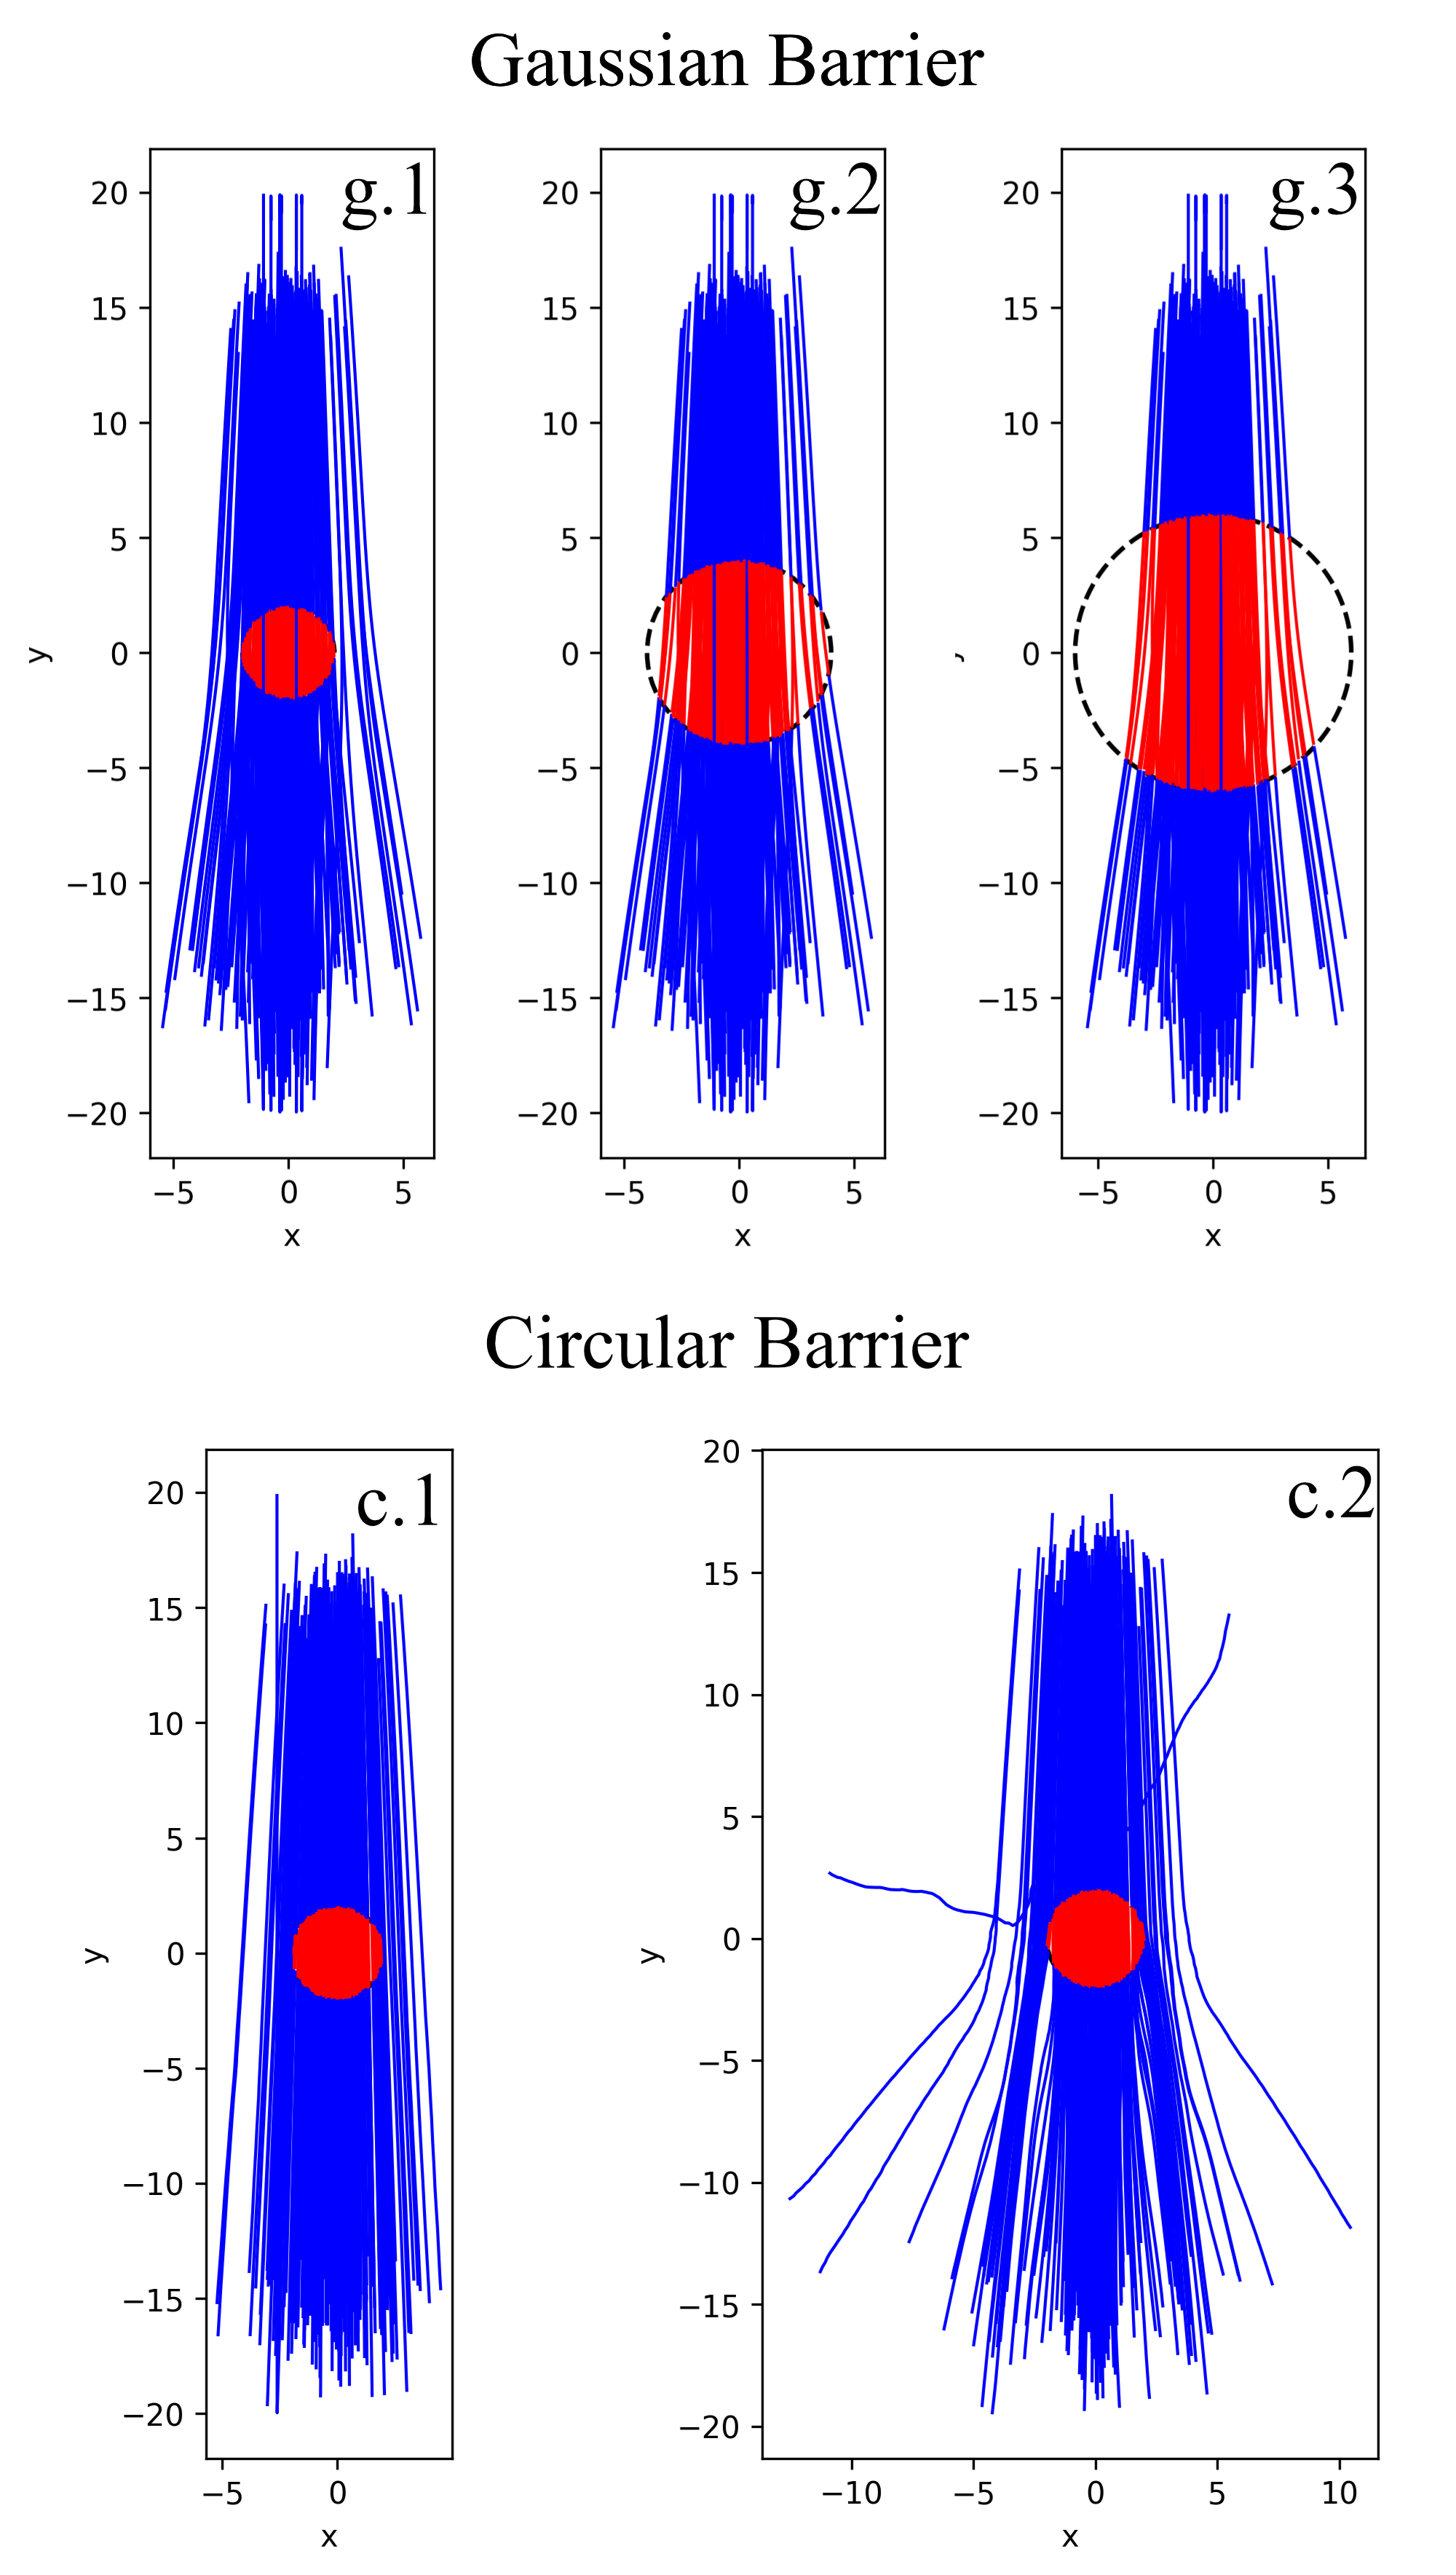
\includegraphics[width=1\linewidth]{Figures//2dspin/bohmian_paths.png}
    
    \caption{Bohmian Trajectories for Gaussian (g) and circular pathways (c). Parts of the pathways that are falling within the barrier are colored red. Gaussian barriers have well defined boundary. Portrayed are boundaries equal to 2R=[$1\sigma$,$2 ln(2) \sigma$,$3\sigma$], respectively for [g.1, g.2, g.3]}. $2 ln(2) \sigma$ corresponds to FHWM of the laser beam intensity profile.
    \label{fig:bohmiantrajectories}
\end{figure}

% Weak Field Analysis

\begin{figure}
    \centering
    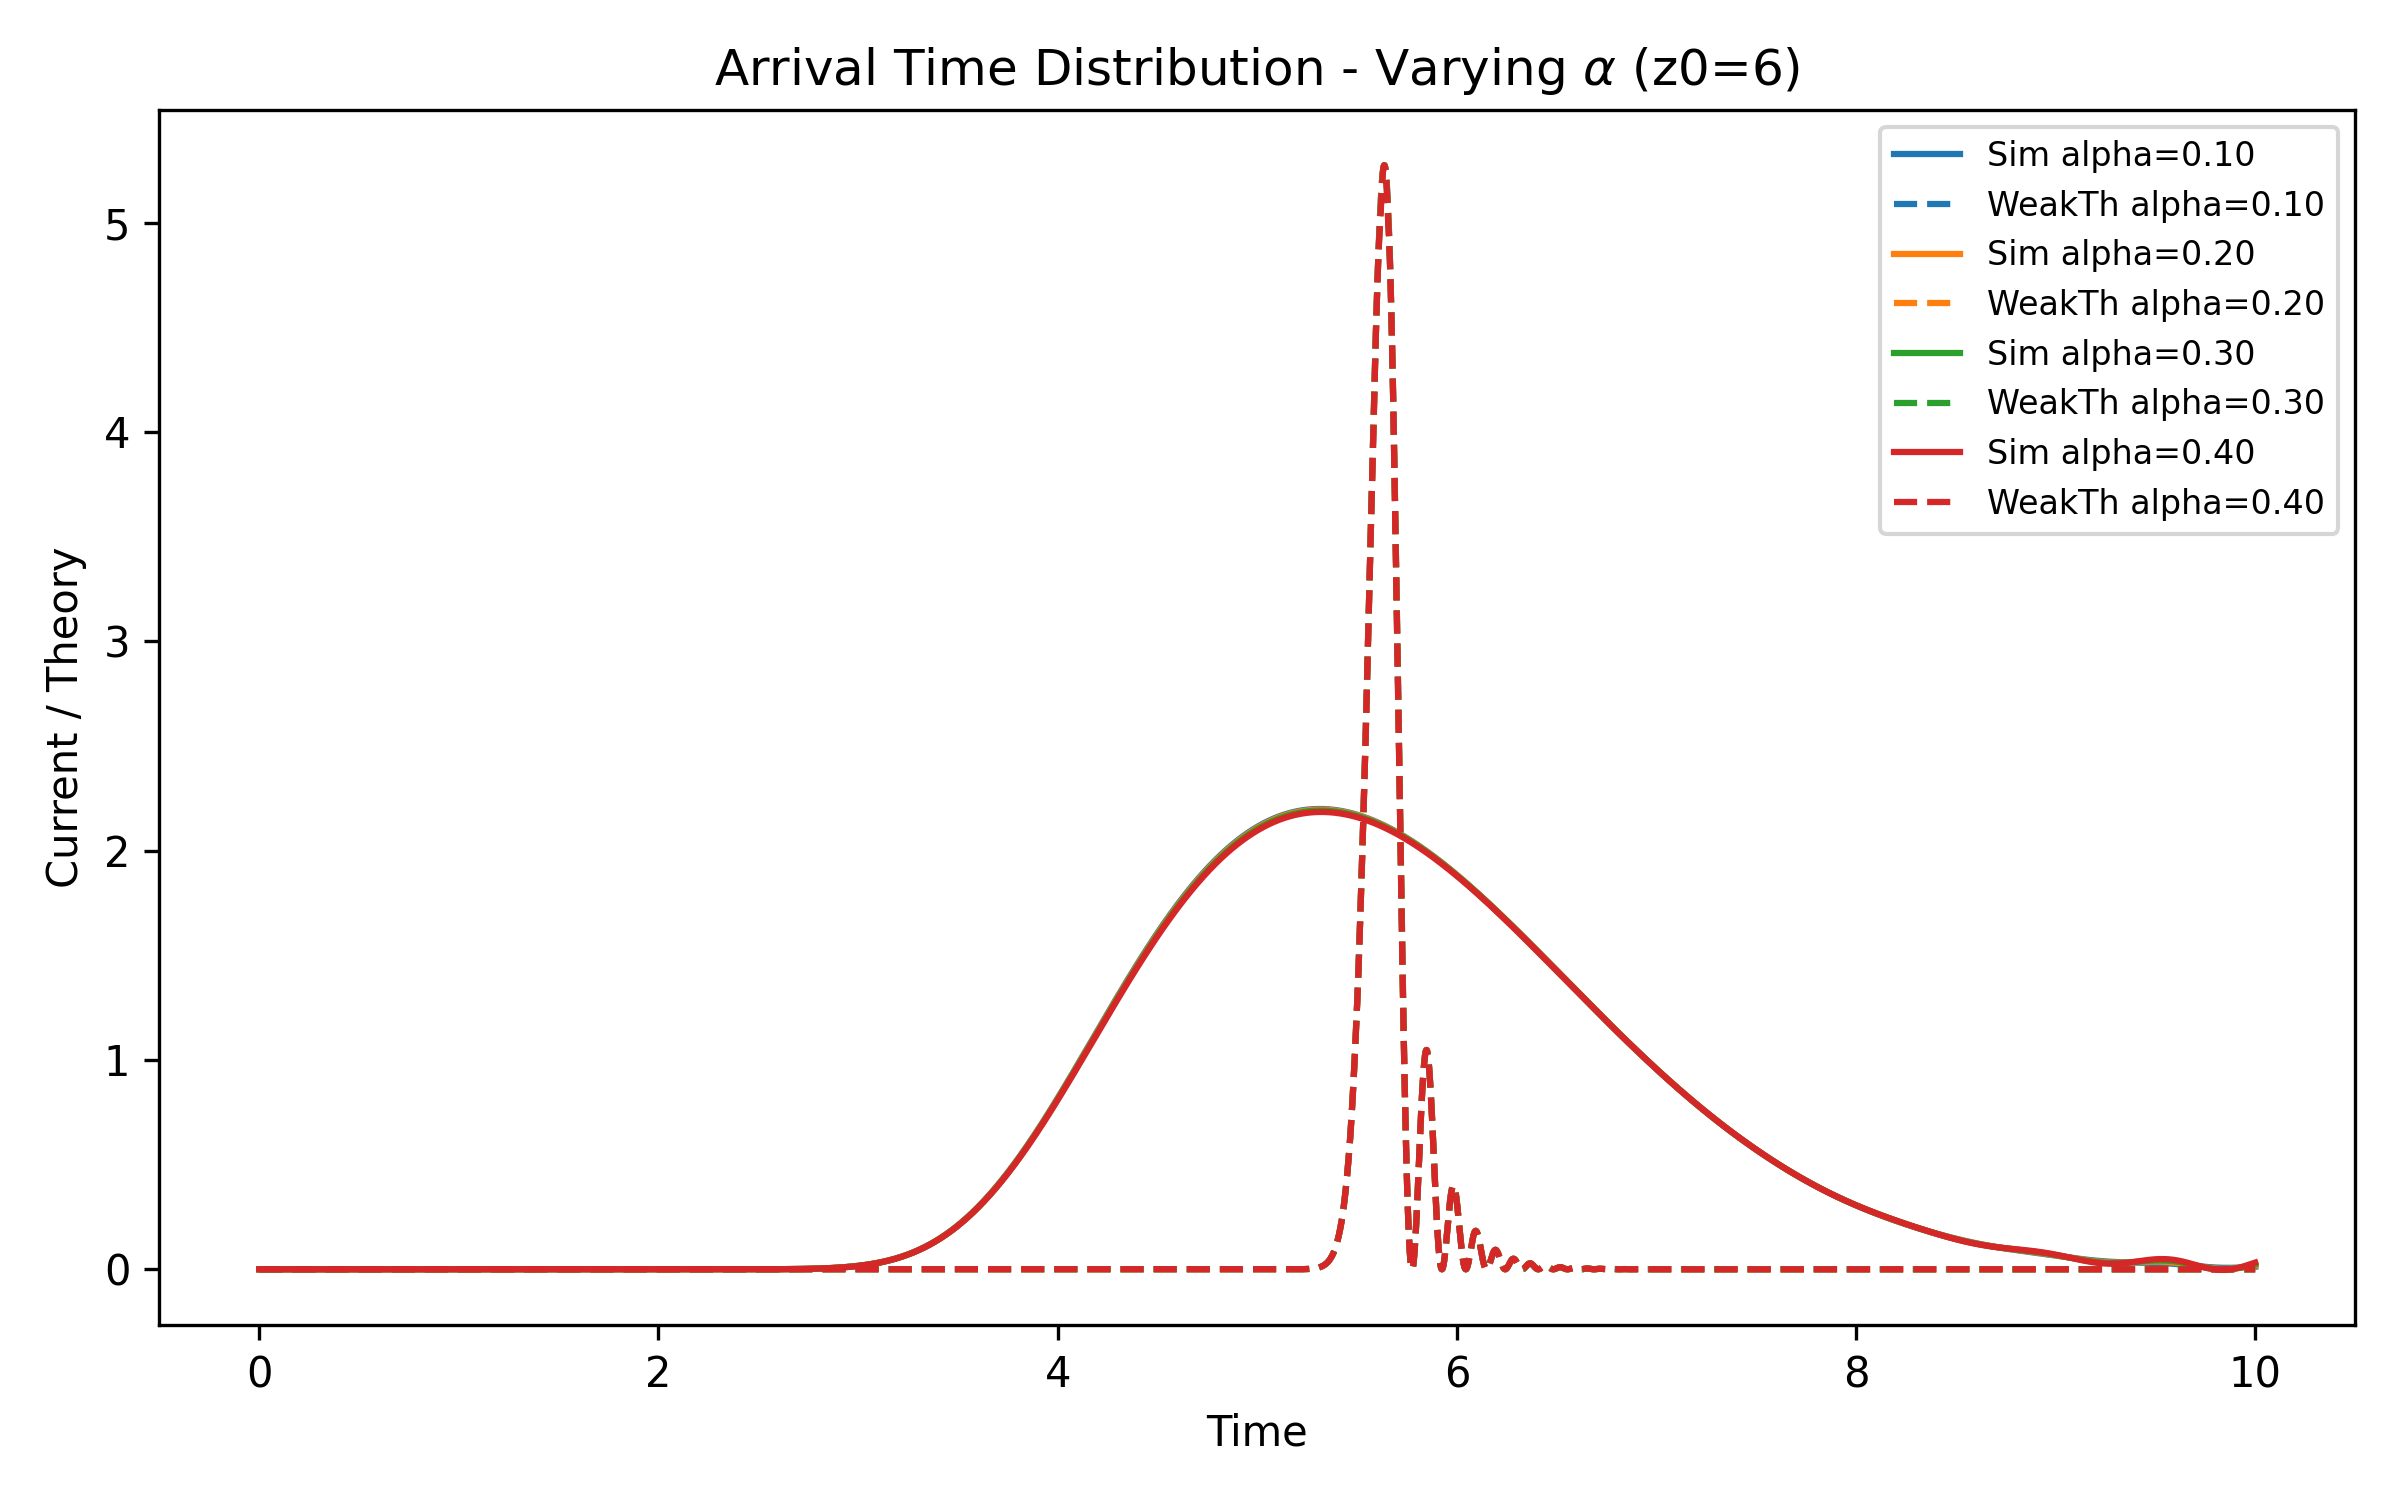
\includegraphics[width=1\linewidth]{Figures//WeakBarrier/varying_alpha.png}
    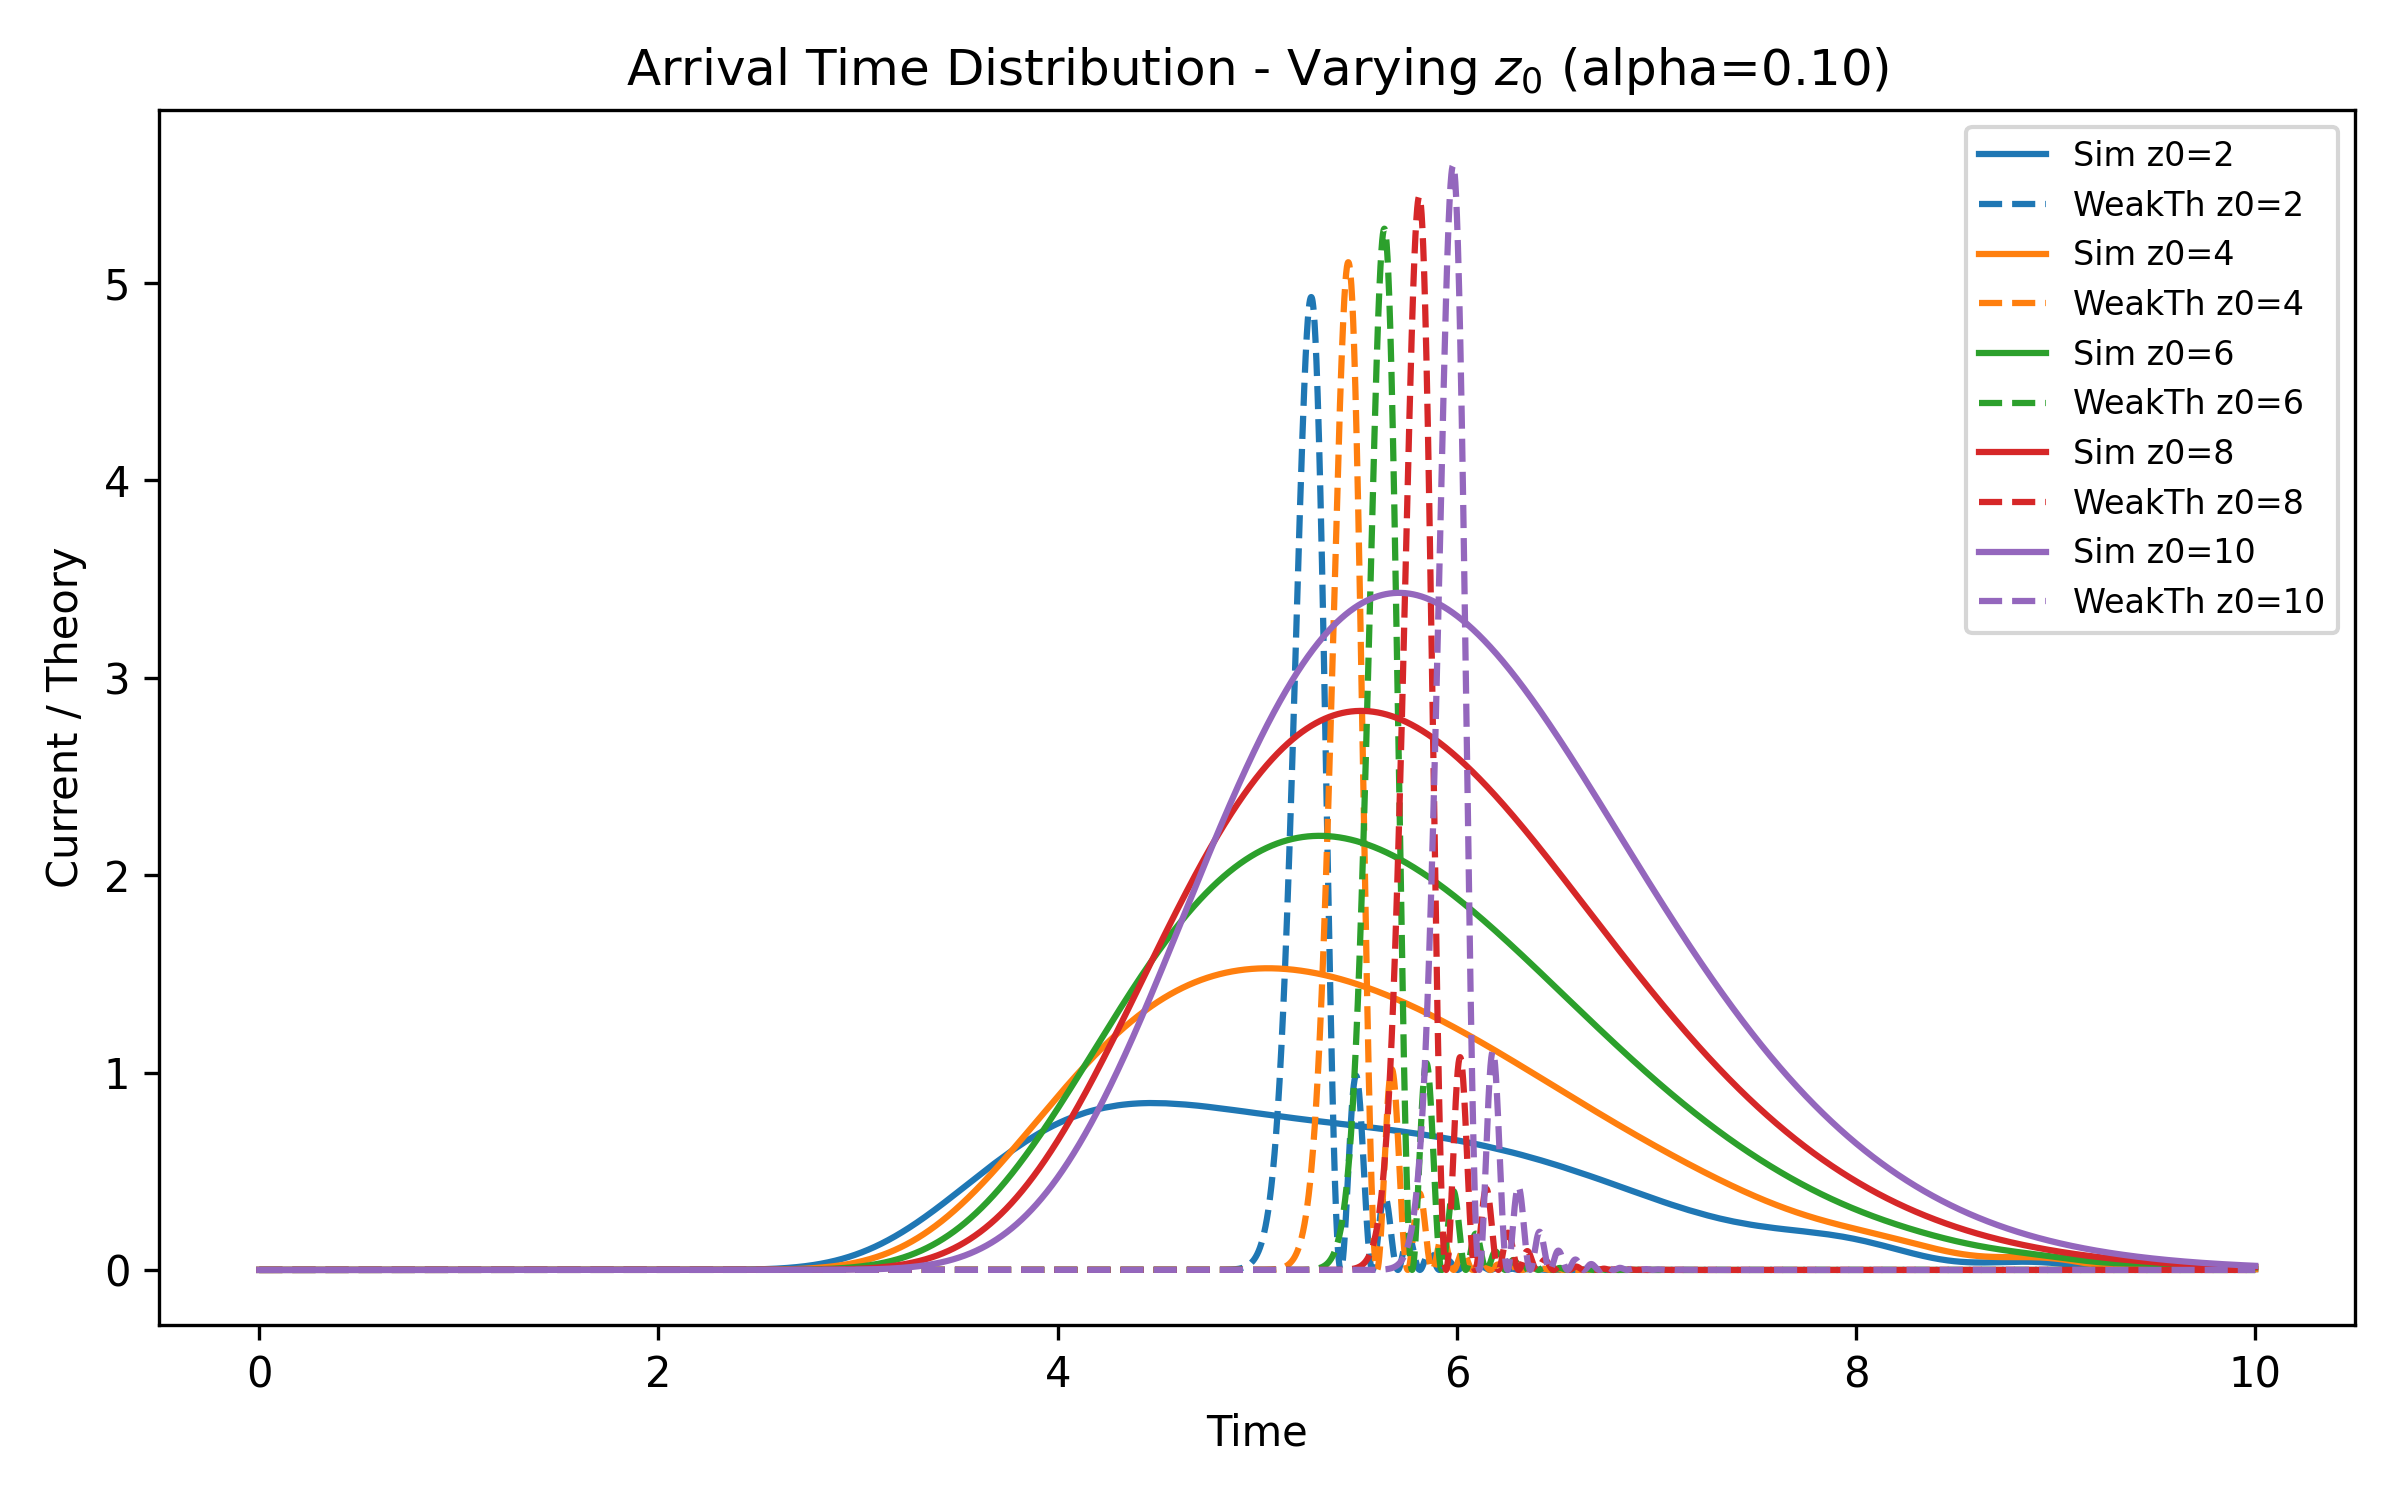
\includegraphics[width=1\linewidth]{Figures//WeakBarrier/varying_z0.png}
    
    \caption{Comparing Weak Barrier Theory vs Bohmian Simulations. The overal "bulk" of the arrival time matches, but the resonant peaks are nowhere to be seen. Further, the peaks for the weak theory don't spread out on the x-axis (time) as the particle is dropped from a higher height, which is to be expected from the general form of the TDSE.}
    \label{fig:peak_barrier_vs_secs}
\end{figure}

\begin{figure}
    \centering
    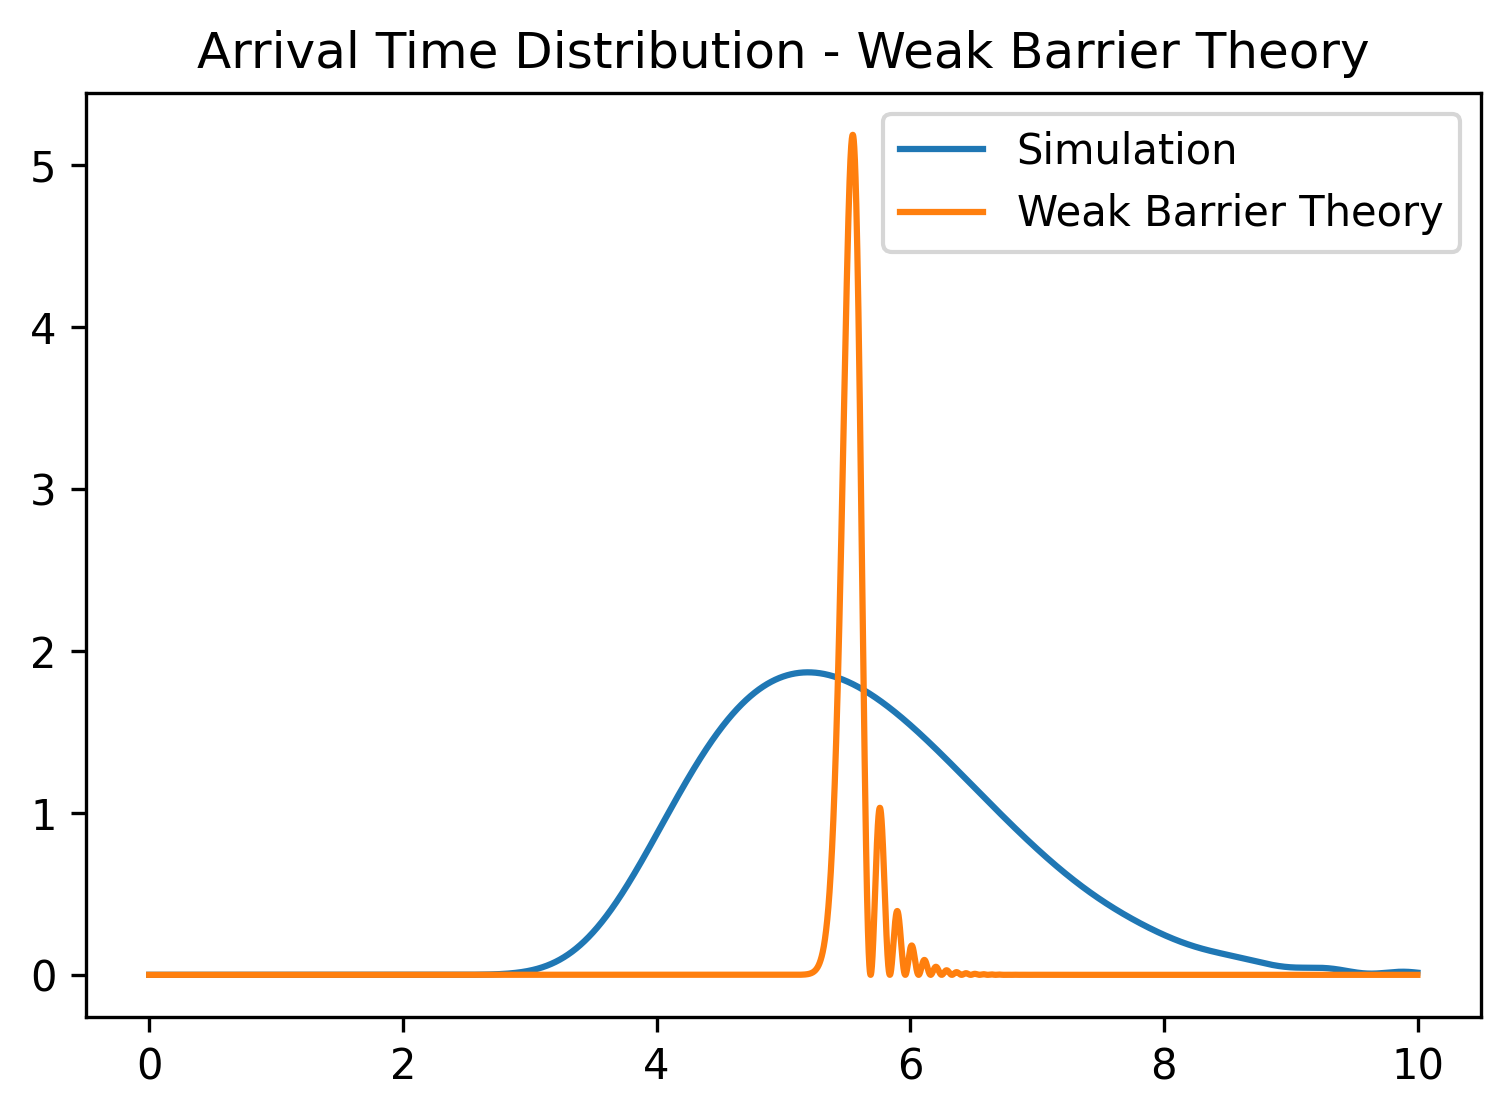
\includegraphics[width=1\linewidth]{Figures//WeakBarrier/5e99d081-68c5-496a-81de-d96909010d37.png}
    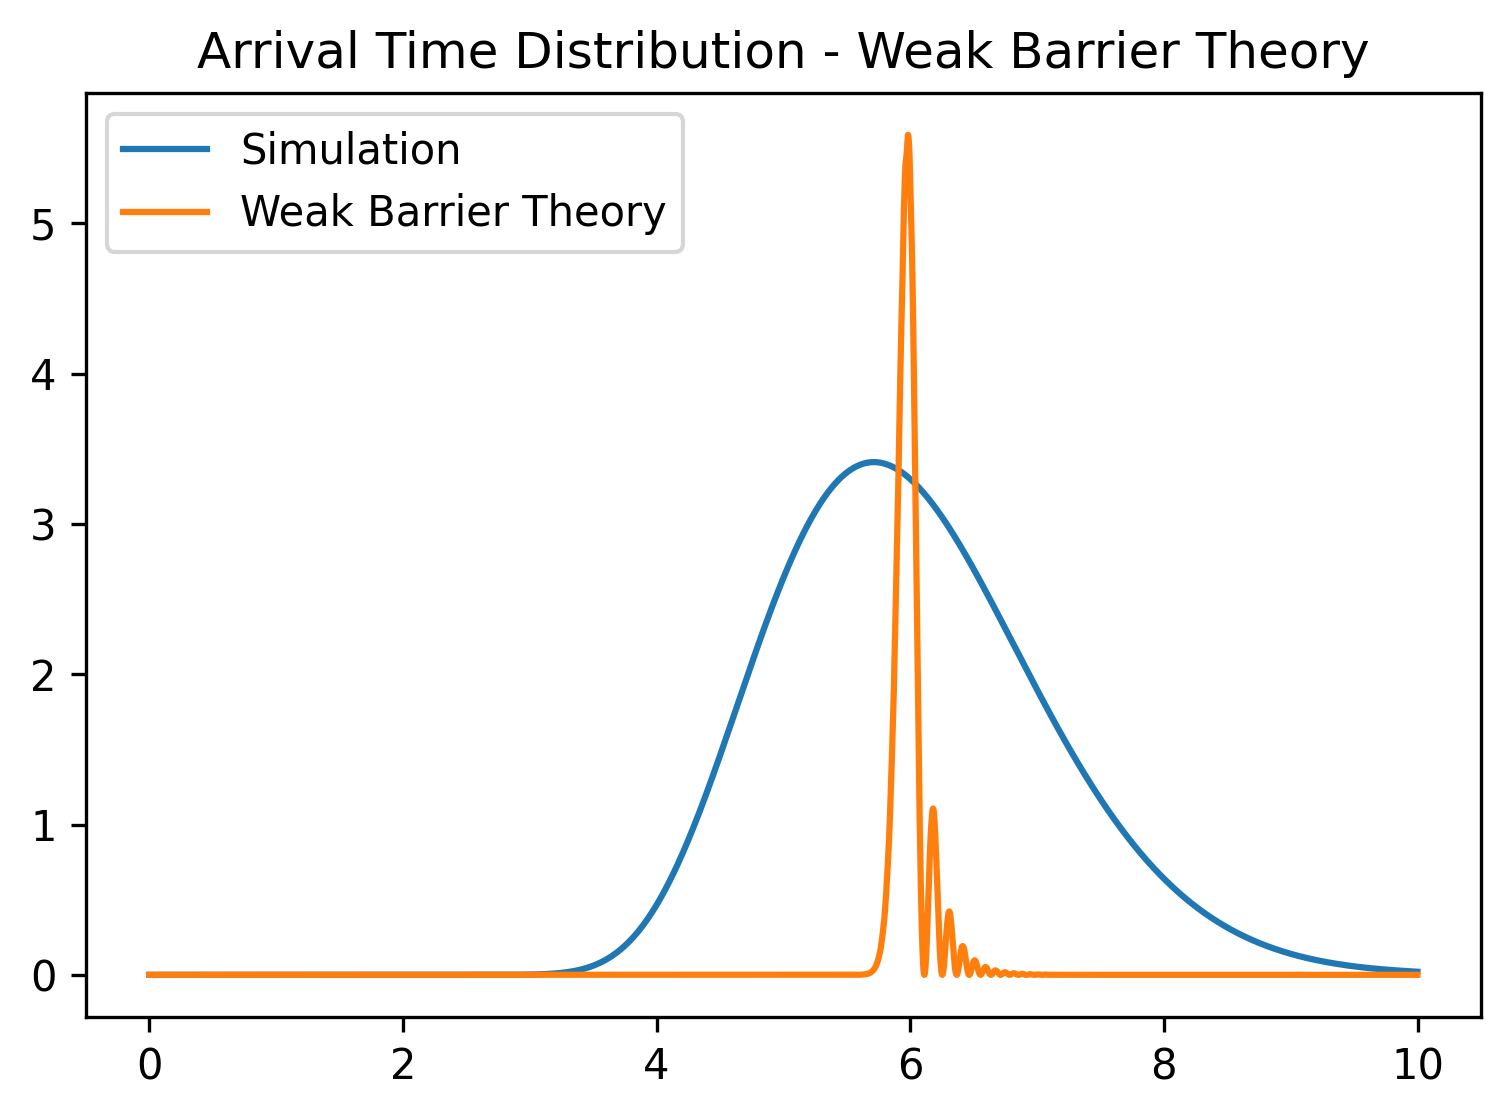
\includegraphics[width=1\linewidth]{Figures//WeakBarrier/e1718b30-5126-45b4-9644-ec9806071d7f.png}
    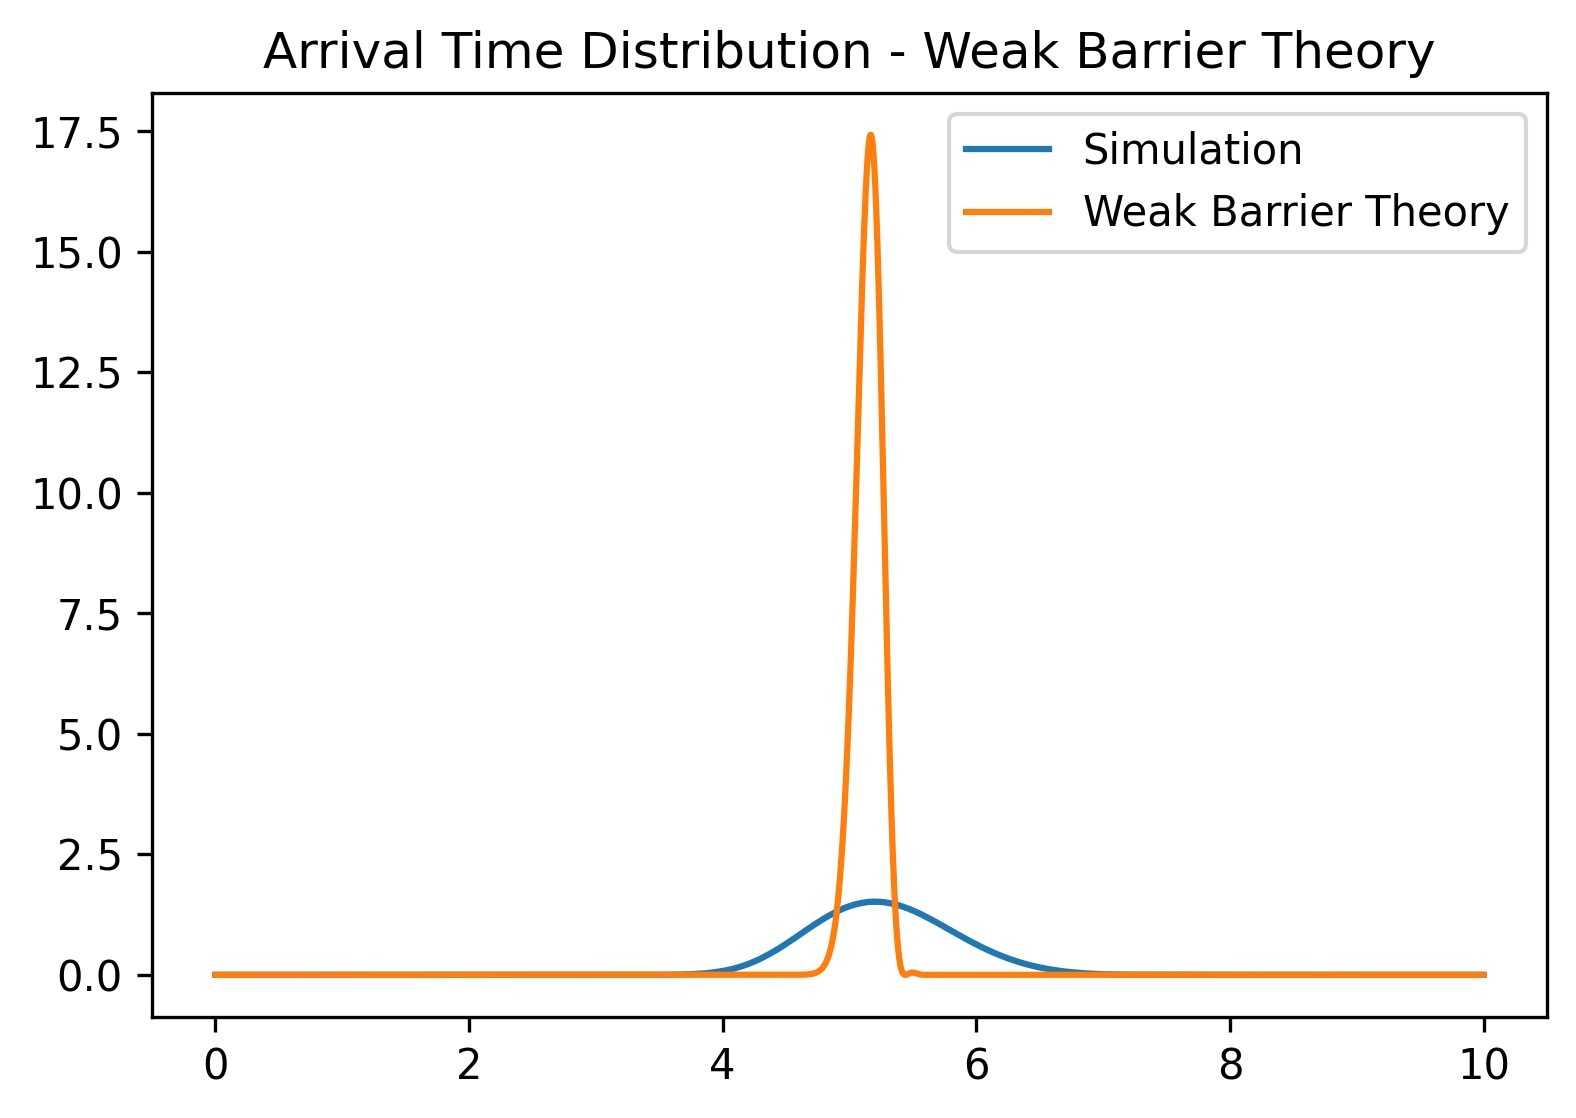
\includegraphics[width=1\linewidth]{Figures//WeakBarrier/f745cad5-c635-419c-b9f7-5867d8c5cb00.png}
    
    \caption{Comparing Weak Barrier Theory vs Bohmian Simulations. The overal "bulk" of the arrival time matches, but the resonant peaks are nowhere to be seen. Figures correspond to different barrier strengths, width, and heights, whose absolute values are irrelevant to specify in the current scope.}
    \label{fig:peak_barrier_vs_secs}
\end{figure}

\begin{figure}
    \centering

    \begin{subfigure}[b]{0.8\linewidth}
        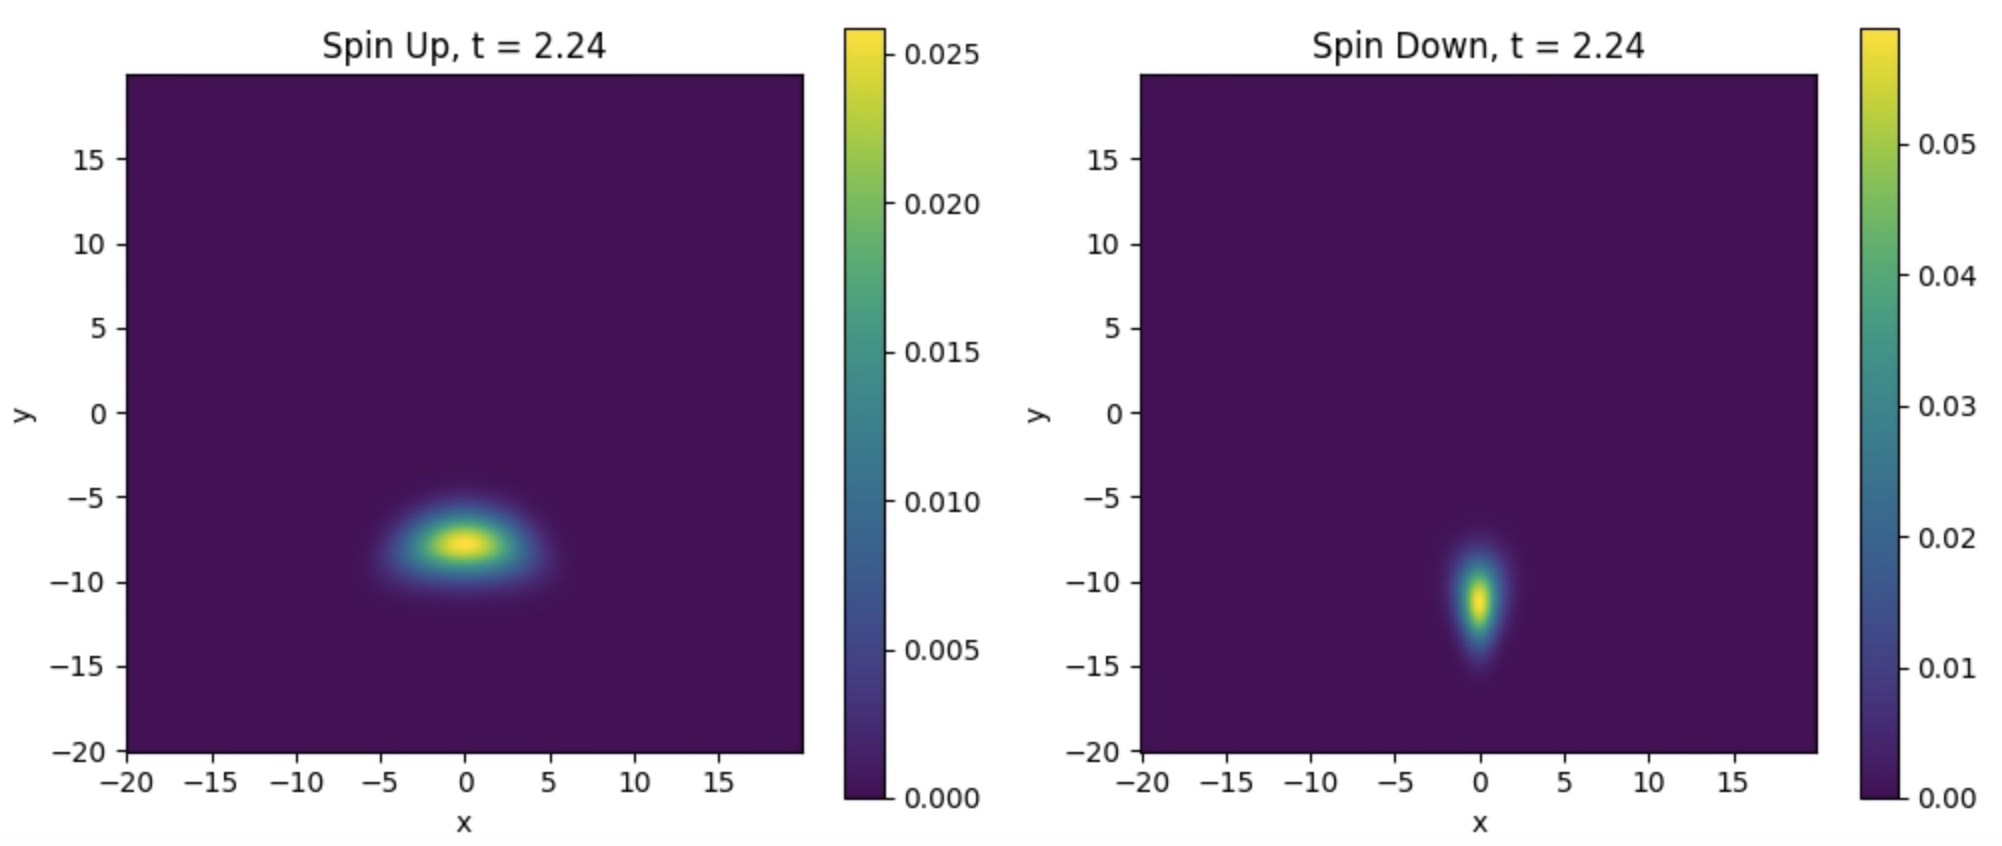
\includegraphics[width=\linewidth]{Figures//2dspin/Screenshot 2025-05-18 at 01.34.21.png}
        \caption{First snapshot}
    \end{subfigure}
    
    \caption{This figure illustrates how a 2D particle in free fall, made of $\psi_{\uparrow}$ and $\psi_{\downarrow}$ in superposition, across a \textbf{strong Gaussian magnetic field} reacts, is deformed. Notice the clearly smooth spread of the wave function, as opposed to Strong Circular Barriers like in \ref{fig:fafwqfqfqfaf12}}
    \label{fig:fafwqfqfqfa}
\end{figure}

\begin{figure*}[t]
    \centering
    \begin{subfigure}[b]{0.8\linewidth}
        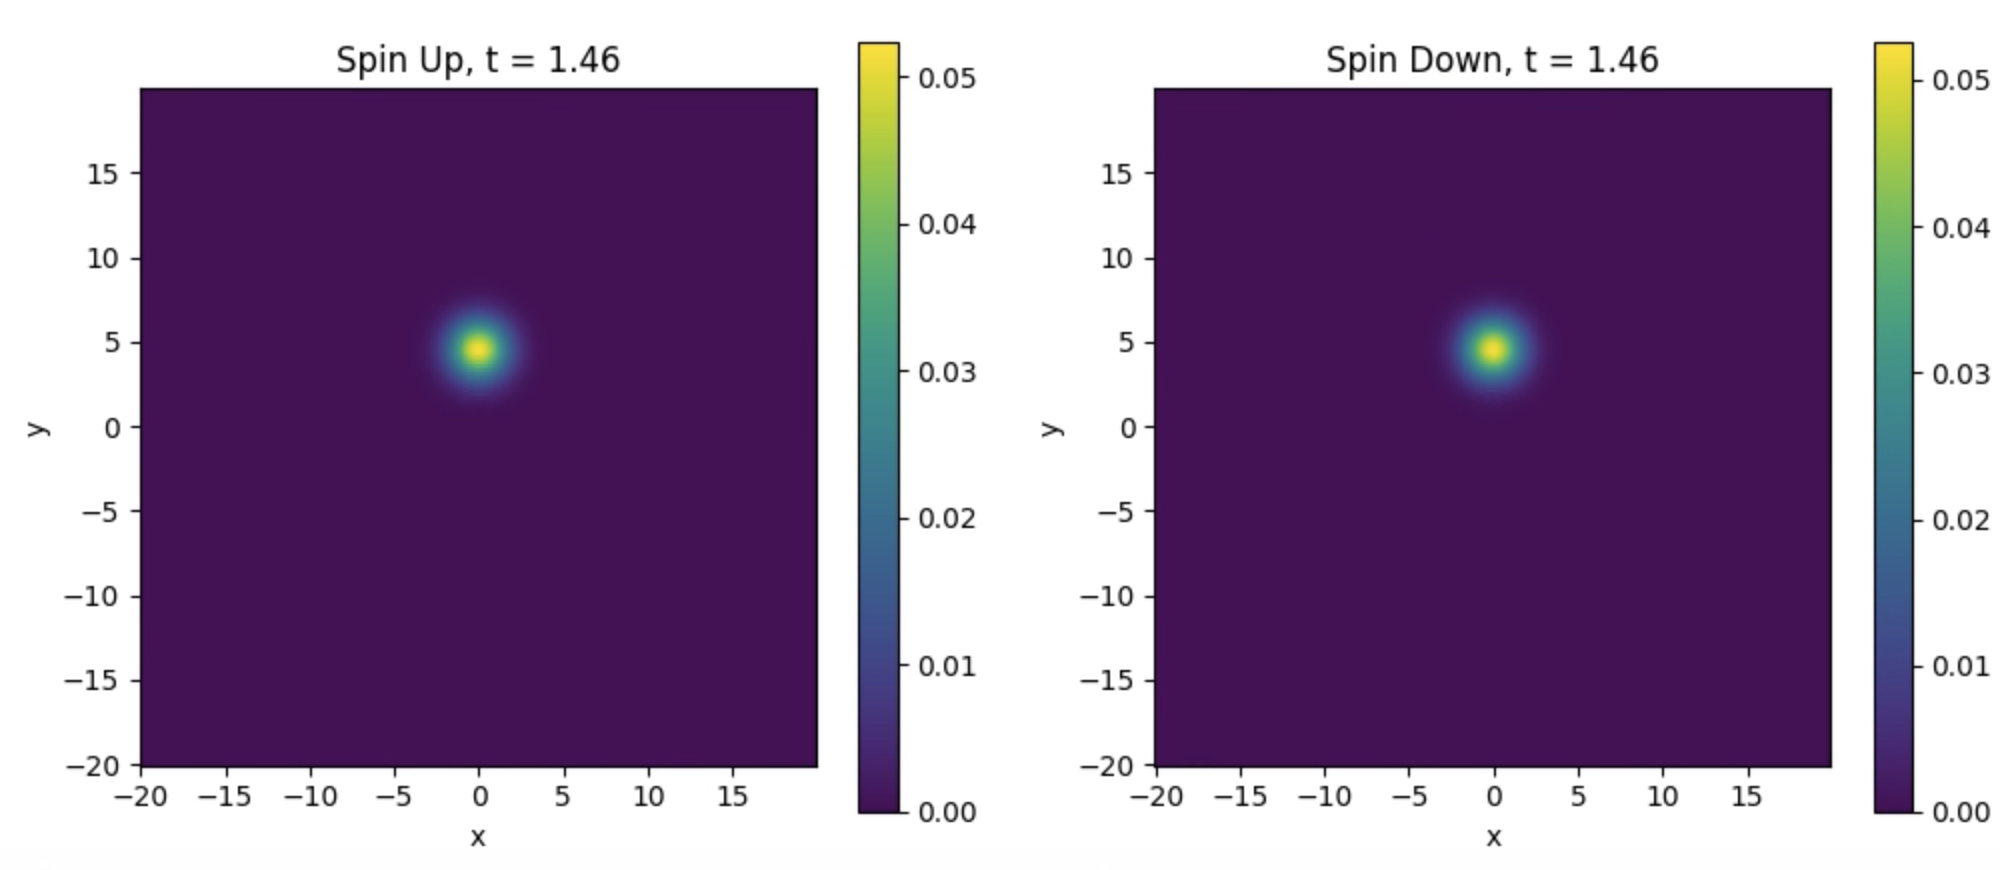
\includegraphics[width=\linewidth]{Figures//2dspin/Screenshot 2025-05-18 at 01.35.22.png}
        \caption{$t=1.46$ seconds}
    \end{subfigure}
    \vspace{0.5em}
    \begin{subfigure}[b]{0.8\linewidth}
        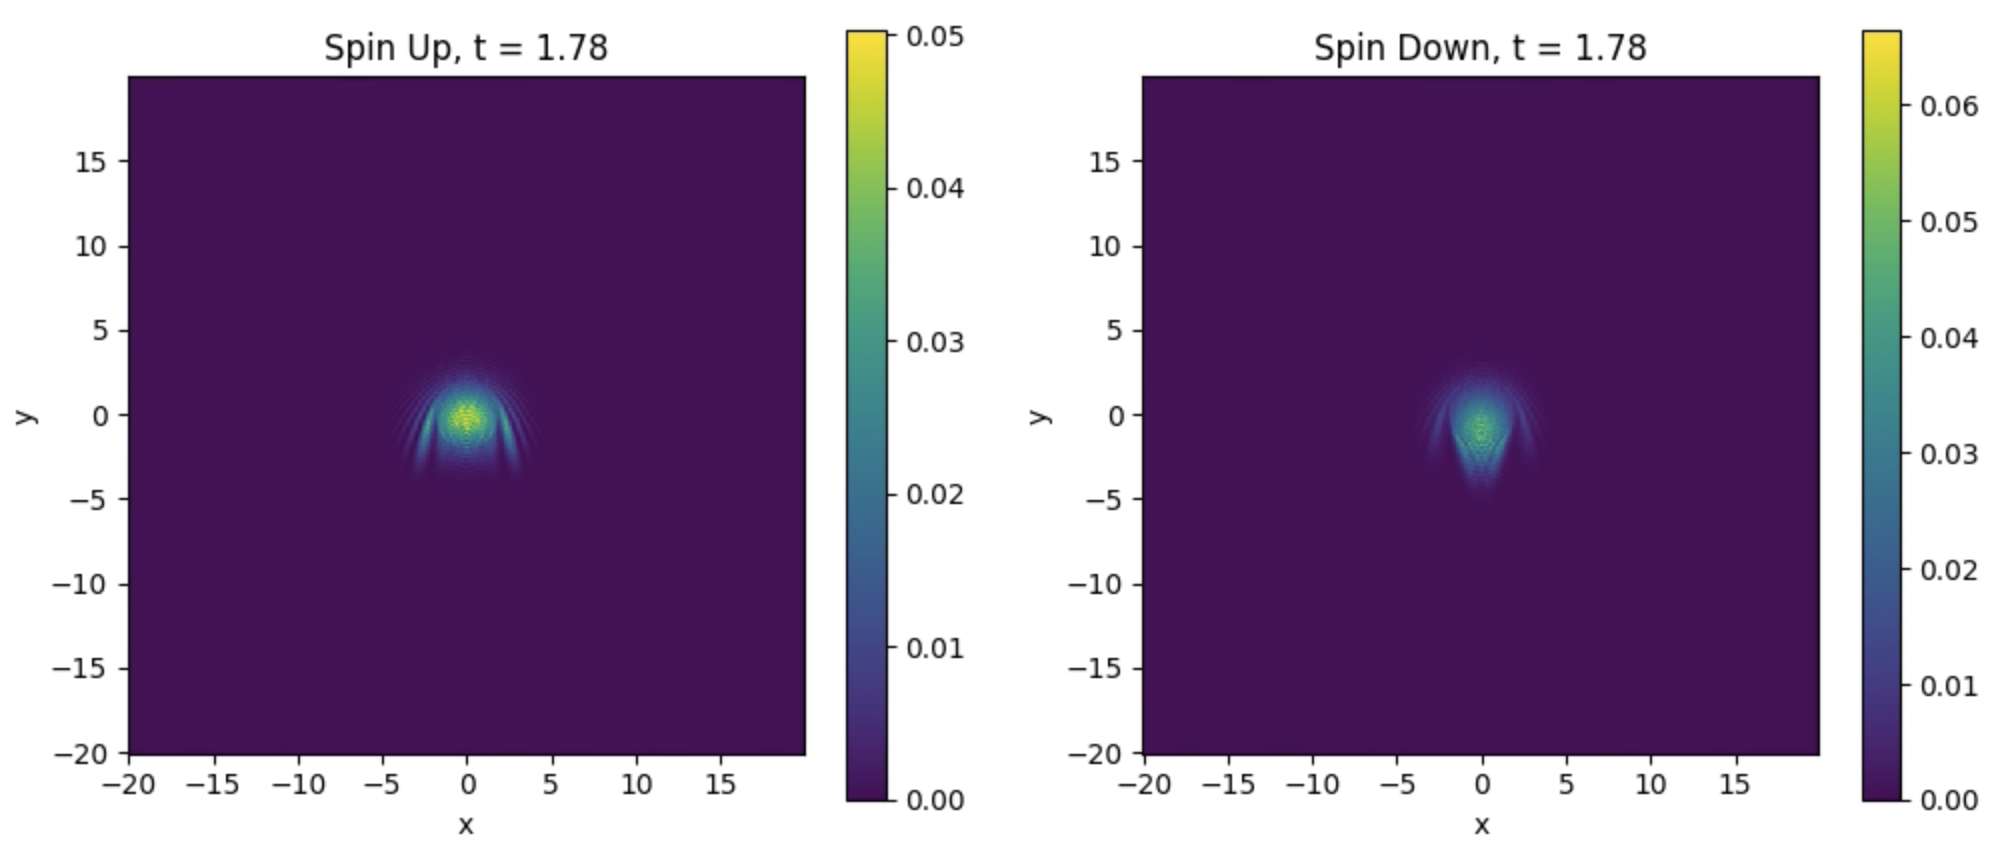
\includegraphics[width=\linewidth]{Figures//2dspin/Screenshot 2025-05-18 at 01.35.35.png}
        \caption{$t=1.78$ seconds}
    \end{subfigure}
    \hfill
    \begin{subfigure}[b]{0.8\linewidth}
        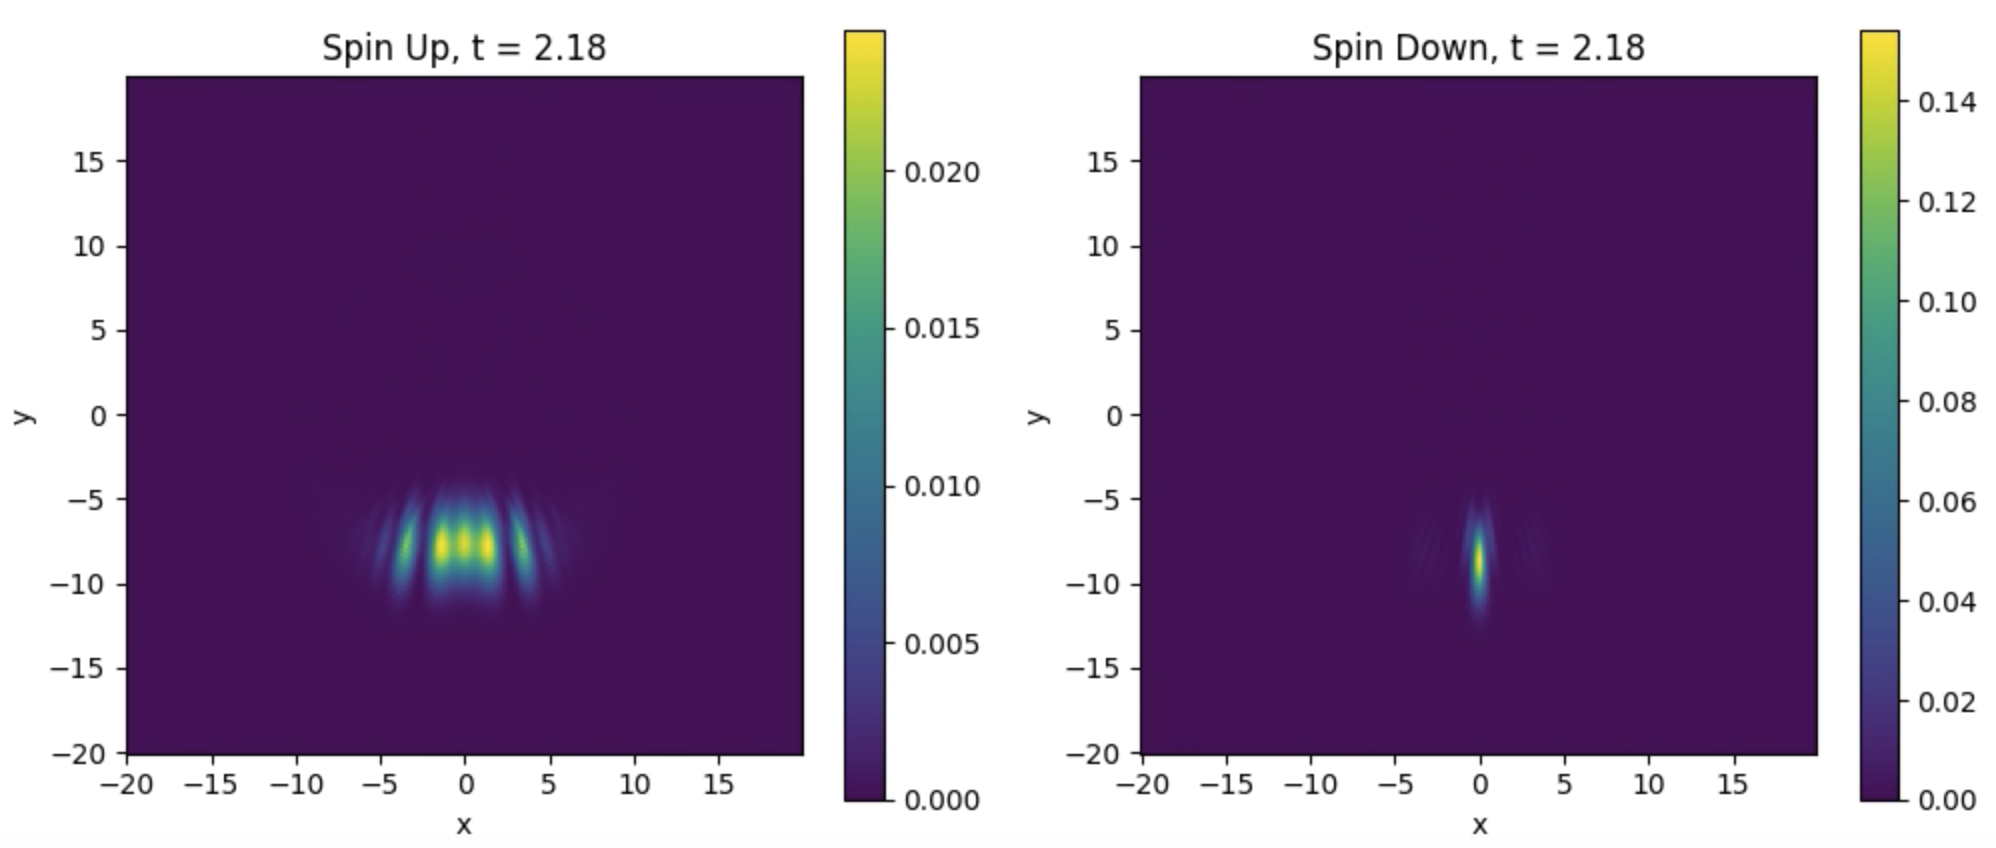
\includegraphics[width=\linewidth]{Figures//2dspin/Screenshot 2025-05-18 at 01.35.50.png}
        \caption{$t=2.18$ seconds}
    \end{subfigure}
    
    \caption{This figure illustrates how a 2D particle in free fall, composed of $\psi_{\uparrow}$ and $\psi_{\downarrow}$ in superposition, across a \textbf{strong  circular magnetic field}. Both $\psi$ components are plotted separately, respectively left and right. (a-c) shows a time evolution of $|\psi|^2$ for a strong circular barrier, revealing Gibbs Phenomena.}
    \label{fig:fafwqfqfqfaf12}
\end{figure*}

